\documentclass[10pt]{article}

%%Fichier de configuration perso
\usepackage{maConfiguration}

\title{%
    \Huge
    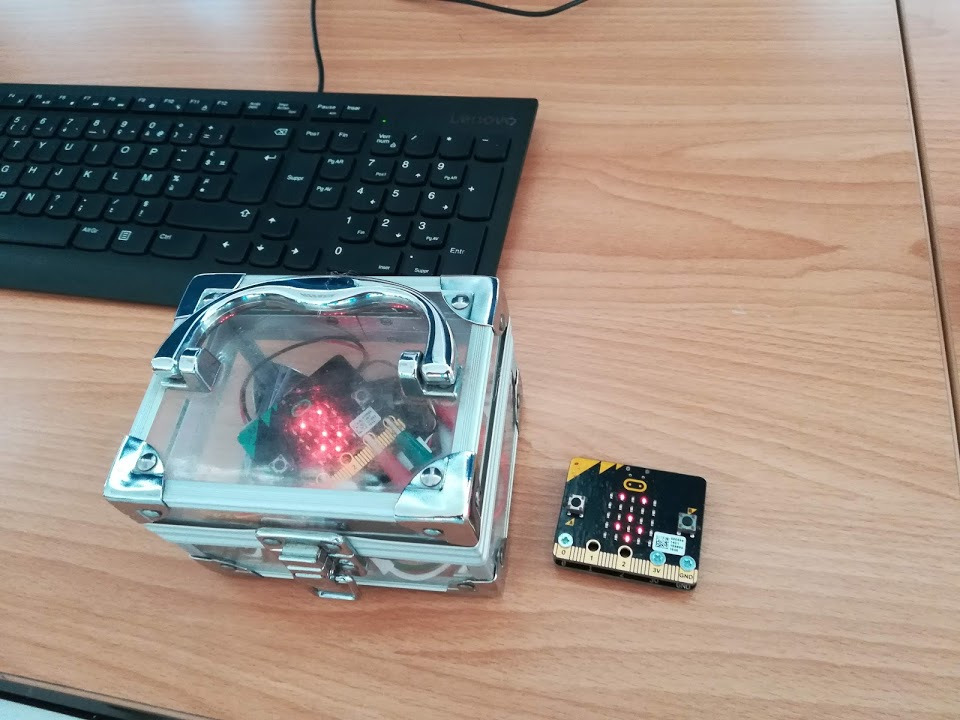
\includegraphics[scale=.2]{mb4}\\[2cm]
    Les objets connectés pour enseigner\\
    l'algorithmique\\
    en lycée professionnel}
\author{%
    Groupe InEFLP\\
    \href{http://url.univ-irem.fr/ineflp}{
\includegraphics[height=2cm]{fig-logo-ineflp}}\\
    de l'IREM\footnote{Institut de Recherche sur l'Enseignement des Mathématiques} de Marseille
    }
\date{\today}



\begin{document}



%%% Titre
\pagecolor{orangeamu!25}
\maketitle\thispagestyle{empty}


%%% Sommaire
\newpage\pagecolor{orangeamu!10}
\tableofcontents


%%% À propos de la brochure
\newpage\pagecolor{bleuamu!10}
% \pagestyle{plain}

\section{À propos de cette publication}



\subsection{Pourquoi les objets connectés?}


Alors que dans certaines disciplines le temps commence à manquer pour traiter l'ensemble du programme, certains évoquent déjà l'idée d'en faire plus !

En effet, les enseignants utilisent déjà les outils numériques. Par exemple, dans les classes de mathématiques, l'utilité du tableur et de GeoGebra n'est plus à démontrer. Jusqu'à l'introduction de l'algorithmique, ces deux logiciels efficaces et maîtrisés par les enseignants étaient amplement suffisants.
Est-ce donc juste un effet de mode de faire cours avec les robots (Thymio, Mbot), les objets  programmables et connectés (Arduino, \mb, STM education, Raspberry Pi) ou est-ce une nouvelle façon d'aborder notre enseignement?
Ces nouvelles possibilités technologiques, forcément chronophages, nous permettront-elles de traiter un contenu disciplinaire exigeant dans un cadre institutionnel contraignant?

Nous n'avons bien sûr pas toutes les réponses à ces questions mais nous pensons que lorsqu'il est accompagné de certains de ces outils, notre enseignement a beaucoup à y gagner.

L'introduction de l'algorithmique en lycée professionnel nous interroge. Longtemps il nous a semblé impensable et inenvisageable d'avoir à enseigner un langage de programmation comme Python auprès d'un public d'élèves globalement en difficulté avec les mathématiques. Fort de ce constat, nous avons cherché les moyens de lier les mathématiques à la logique et au raisonnement algorithmique. C'est pourquoi nous avons exploré les potentialités des objets connectés.


\begin{formule}
	Notre postulat est double. Nous pensons que :
		\begin{itemize}
			\item grâce à des situations réelles et concrètes, les objets connectés facilitent la mise en activité de tous les élèves ;
			\item grâce à des activités simples mais évolutives centrées autour de réalisations matérielles, la dimension affective du travail est valorisée.  Soyons fous et espérons que l'élève tisse une histoire personnelle avec l'activité, qu'il soit fier du travail accompli et  qu'il prenne également du plaisir à expliquer et à montrer ses réalisations.
	\end{itemize}
\end{formule}


En devenant de plus en plus simples, accessibles et facilement utilisables, les objets connectés permettent d'aborder des contenus disciplinaires et de développer des compétences transversales essentielles pour l'élève.

En travaillant à partir des objets connectés, la situation de départ est plus concrète et l'objectif à atteindre suffisamment clair pour l'élève. Plus ou moins guidé selon son niveau d'expertise technique, il est alors libre dans sa démarche.
Avec des interfaces de programmation accompagnées parfois de simulateurs, la démarche par essais et erreurs a ici toute sa place.
Par ailleurs, l'élève devra clarifier sa pensée avant de verbaliser ses idées en langage naturel. Il pourra ainsi proposer et élaborer un modèle acceptable par la machine pour enfin traduire son algorithme en se pliant à la rigueur du langage de programmation. 

Effectuant régulièrement des va-et-vient entre abstraction et réalité, cherchant à valider son algorithme à partir d'un visuel ou d'une exploitation des résultats, l'élève entre progressivement dans la modélisation.

Les scénarios proposés dans cette brochure permettent tout cela : une approche des mathématiques et des sciences qui laisse la place à l'expérimentation : manipulation, programmation et auto-validation. 




\pagebreak

\subsection{Qui sommes-nous?}

Nous sommes des enseignants de maths/sciences regroupés au sein d’un groupe de recherche de l'IREM de Marseille.

\begin{center}
	\href{http://url.univ-irem.fr/ineflp}
	{
\includegraphics[width=0.5\linewidth]{res/fig-logo-ineflp.png}}
\end{center}

Notre groupe, Innovation, Expérimentation et Formation en Lycée Professionnel (InEFLP) consacre une partie de son travail à l’enseignement de l’algorithmique en classes de lycée professionnel. Dans le cadre de cette recherche, nous explorons les objets connectés tels que Arduino, \mb, \st ou mbot.





\subsection{Liens utiles}
\begin{description}
    \item[Page du groupe InEFLP]  ~\\
        \url{http://url.univ-irem.fr/ineflp}
    \item[IREM de Marseille] Site académique de l'IREM de Marseille\\
        \url{http://url.univ-irem.fr/mars}
    \item[Portail des IREM] Site national des IREM\\
        \url{http://www.univ-irem.fr/}
    \item[Formation à l'algorithmique LP et SEGPA]
        Padlet de utilisé lors de nos formations académiques\\
        \url{http://url.univ-irem.fr/stage-algo}
    \item[Collecte de ressources pour \mb]
        Padlet sur \mb utilisé en formation\\
        \url{http://url.univ-irem.fr/algo2017-microbit}
    \item[Brochure sur \mb]
        Publication de la \href{http://www.univ-irem.fr/spip.php?rubrique18}{C2i TICE} pour une prise en main de \mb\\
        \url{http://url.univ-irem.fr/c2it-mb-t1-pdf}
    \item[Description \mb] Fiche sommaire de description de \mb\\
        \url{http://url.univ-irem.fr/ineflp-microbit}
    \item[Site IREM dédié à \mb] Site de ressources sur \mb du groupe\\
        \url{http://url.univ-irem.fr/o}
\end{description}


\begin{center}
    \href{http://url.univ-irem.fr/ineflp}
    {
\includegraphics[width=0.1\linewidth]{res/fig-ineflp-qr.png}}
\end{center}




%%% Généralités
\newpage\pagecolor{bleuamu!10}
% \style{plain}

\section{À propos de la carte \mb}


\mb est un microcontrôleur développé au Royaume-Unis.
Par ses caractéristiques techniques et ses interfaces
pédagogiques, cet objet possède un fort potentiel pour
l’enseignement de l’algorithmique.



\begin{wrapfigure}{r}{4cm}
	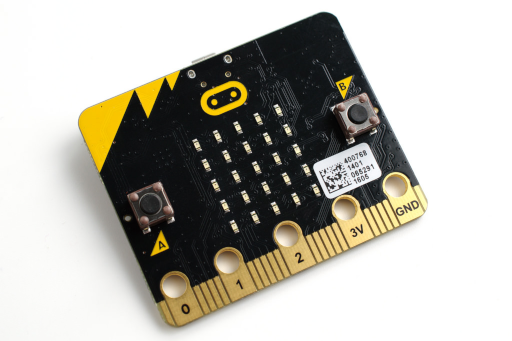
\includegraphics[width=\linewidth]{res/mb-ap-01.png}
	\legend{Carte \mb}
\end{wrapfigure}

Après un bref rappel historique, nous expliquerons plus en détail les caractéristiques propres de cet objet. Nous mettrons ensuite en avant la facilité de mise en œuvre en formation puis nous poursuivrons en donnant un premier aperçu de l’intérêt pédagogique de \mb.

\subsection{Bref historique}


Le développement de \mb s’inscrit dans le cadr d’une politique volontariste de développement de l’apprentissage de la programmation. L’objectif premier visait à équiper tous les élèves de 11/12 ans du Royaume-Unis ainsi que leur enseignant. Maintenant que c’est chose faite, le reste du monde peut en profiter aussi.

% \begin{wrapfigure}[12]{r}{5cm}
%     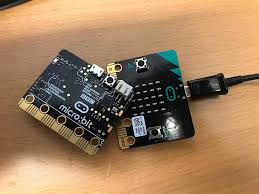
\includegraphics[width=\linewidth]{res/mb-ap-03}
%     \legend{Cartes \mb branchée en USB}
% \end{wrapfigure}


La BBC\footnote{Make It Digital - The BBC micro:bit. (s. d.). Consulté 29 mars 2017, à l’adresse \url{http://www.bbc.co.uk/programmes/articles/4hVG2Br1W1LKCmw8nSm9WnQ/the-bbc-micro-bit}} est le moteur de ce projet. 30 ans après sa première distribution d’ordinateurs aux enfants britanniques\footnote{BBC Micro. (2016, septembre 20). In Wikipédia. Consulté à l’adresse \url{https://fr.wikipedia.org/w/index.php?title=BBC_Micro&oldid=129763631}}, “la Vieille Dame” remet ça aujourd’hui. La BBC utilise ses moyens de diffusions pour promouvoir et accompagner les utilisateurs, notamment en proposant des émissions de TV dédié à cet objet sur un mode ludique et divertissant. Sur les 29\footnote{Partners. (s. d.). Consulté 29 mars 2017, à l’adresse \url{https://www.microbit.co.uk/partners}} partenaires de ce projet, se trouvent entre autres Microsoft\footnote{The BBC micro:bit and Microsoft - Microsoft Research. (s. d.). Consulté 29 mars 2017, à l’adresse \url{https://www.microsoft.com/en-us/research/project/the-bbc-microbit-and-microsoft/}} pour une partie logiciel et interface de programmation, ARM\footnote{Ltd, A. R. M. (s. d.). ARM | Innovation Hub - BBC micro:bit. Consulté 29 mars 2017, à l’adresse \url{http://www.arm.com/innovation/products/microbit.php}} pour la construction des processeur et la partie matériel, et Samsung\footnote{Code on the go with Samsung \& micro:bit. (s. d.). Consulté 29 mars 2017, à l’adresse \url{http://www.samsung.com/uk/citizenship/bbcmicrobit.html}} pour un support mobile. C’est donc un projet qui mobilise des acteurs majeurs du numériques et de la communication, prévu pour durer.

% \begin{figure}
%     \center
%     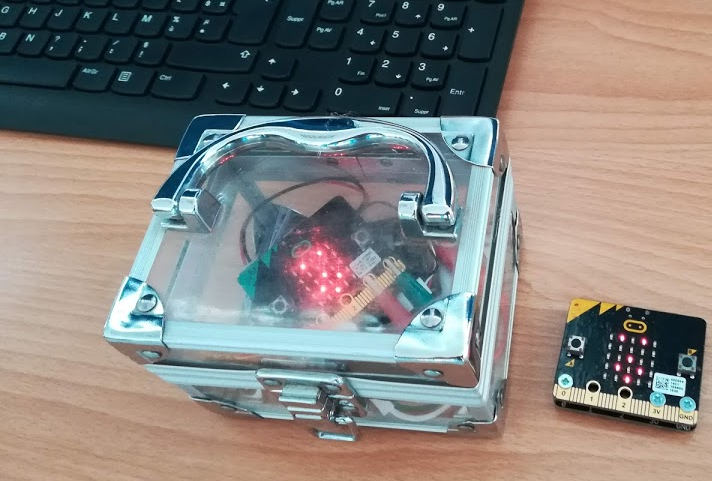
\includegraphics[width=0.5\linewidth]{res/mb-ap-02}
%     \legend{Cartes \mb lors d'un escape game utilisé en formation}
% \end{figure}


\subsection{La carte \mb}

Concrètement de quoi s’agit-il ? On parle ici de microcontrôleur, à savoir une carte électronique programmable pour interagir avec le monde réel.
C’est une version accessible de l’électronique que tout un chacun manipule au quotidien sans se poser de question, par exemple les dispositifs de domotique qui permettent de gérer à distance le chauffage, la sécurité, l’arrosage du géranium… Ou bien plus simplement la bouilloire programmable au degré ${}^{\circ}$C près, la guirlande du sapin qui clignote au rythme de Jingle Bells. 
Ce microcontrôleur permet d’élaborer par exemple un podomètre, un doudou sensoriel, un sismographe rudimentaire\ldots

\begin{figure}
    \centering
    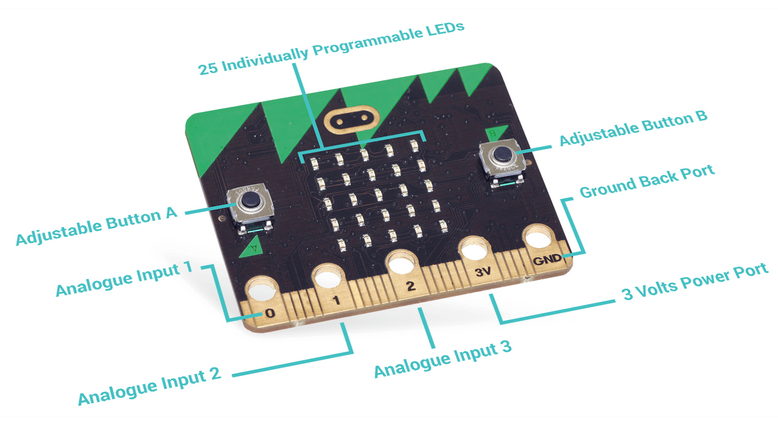
\includegraphics[width=0.49\linewidth]{res/mb-ap-04}
    \hfill
    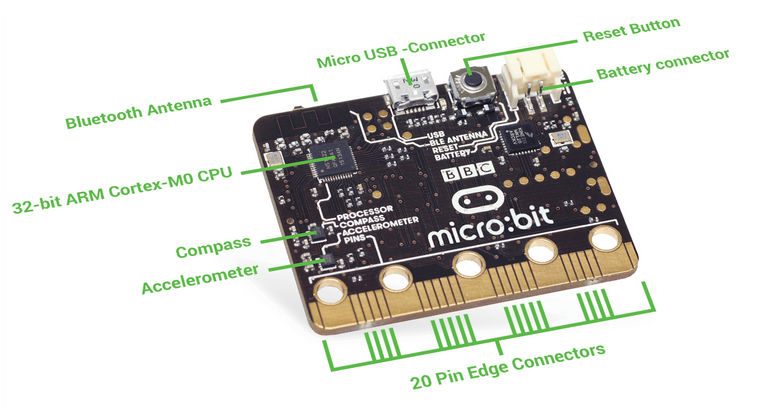
\includegraphics[width=0.49\linewidth]{res/mb-ap-05}
    \legend{Détails des entrées/sorties d'une carte \mb}
\end{figure}

L’interface de programmation est conçue pour être utilisable par un enfant d’une dizaine d’année, c’est donc la simplicité qui prime. On dispose en première approche d’une application internet utilisant le principe de la programmation par bloc, à savoir sur le principe des Blockly que l’on retrouve dans Scratch ou StudioCode. En plus d’une programmation accessible, l’interface propose une simulation de la carte. Ceci permet de voir directement les effets du programme dans l’interface. Pour un usage plus avancé il est notamment possible de programmer avec le langage Python\footnote{Python editor. (s. d.). Consulté 29 mars 2017, à l’adresse \url{http://python.microbit.org/editor.html}} ou Javascript.


\begin{minipage}[b]{0.45\linewidth}
    \vspace{0cm}
    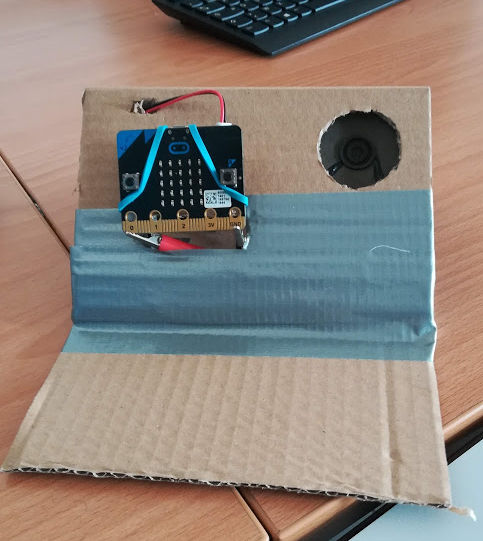
\includegraphics[width=\linewidth]{res/mb-ap-07}
    \legend{Cartes \mb qui fait de la musique (stage 2018)}
\end{minipage}
\hfill
\begin{minipage}[b]{0.45\linewidth}
    Bien entendu de nombreux exemples de projets existent, qu’ils soient issus des émissions BBC ou de la communauté éducative. Sur le site officiel on trouve des idées, des tutoriels, des leçons\footnote{Idées | micro:bit. (s. d.). Consulté 29 mars 2017, à l’adresse \url{http://microbit.org/fr/ideas/}} comme par exemple : une alarme de trousse, un compteur de frappe (au baseball) ou encore des leçons sur l’accélération.
    \vspace{1em}
    \begin{center}
        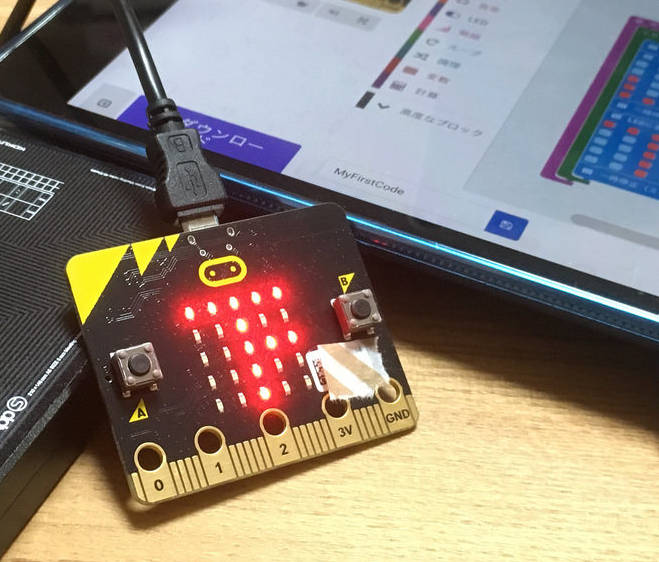
\includegraphics[width=\linewidth]{res/mb-ap-08}
    \end{center}
\end{minipage}


\subsection{Programmer la carte \mb \emph{par blocs}}

\subsubsection{Une interface en ligne}

L’interface de programmation par blocs a été développée en partenariat avec microsoft, elle se trouve en ligne à cette adresse: \url{https://makecode.microbit.org}

Il s’agit donc d’une page internet mais dont le code est mis en cache par le navigateur ce qui signifie qu’elle reste opérationnelle hors ligne.


\begin{remarque}
    À partir de chrome par exemple, il est possible de créer un raccourci sur le bureau.
\end{remarque}



\subsubsection{Un simulateur !}

Le très gros intérêt de cette interface consiste en son simulateur de carte qui permet d’avoir un aperçu du fonctionnement du programme avant même de le télécharger sur la carte.

\begin{figure}[h]
    \centering
    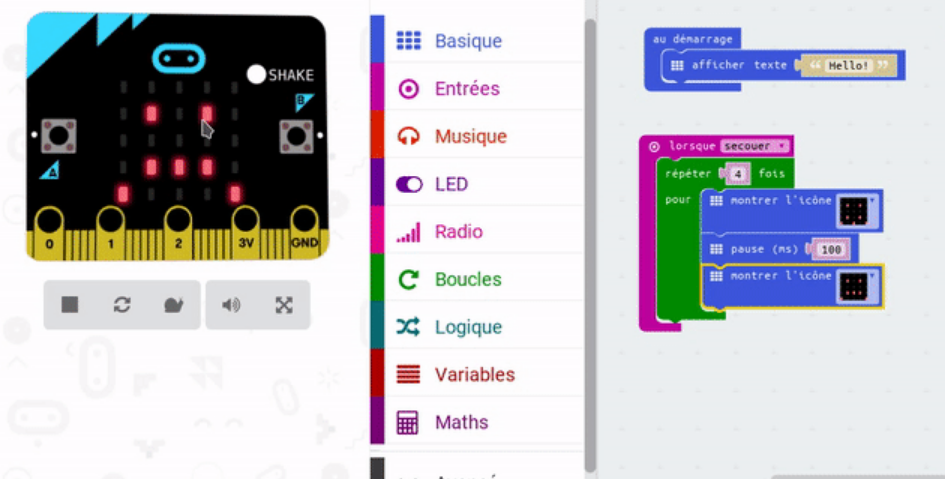
\includegraphics[width=0.75\linewidth]{mb-prog.png}
    \legend{Interface de programmation par bloc qui intègre un \emph{simulateur}}
\end{figure}




\begin{remarque}
    Le simulateur peut ne pas fonctionner hors ligne.
\end{remarque}

\subsubsection{Compilation et enregistrement}

Le téléchargement sur la carte se fait très simplement puiqu’elle est reconnue comme une clé USB. Il suffit donc de cliquer sur Télécharger et de copier le fichier obtenu (.hex) sur la carte.

\subsubsection{Programmation par bloc}

Comme toute interface de programmation par blocs, elle est très intuitive à manipuler. Les premiers programmes se font très simplement et les catégories sont classées par couleurs et par technicité.

\begin{remarque}
    L’interface propose aussi de programmer en javascript, il suffit juste de cliquer sur un bouton pour changer de type de programmation.
\end{remarque}

\subsubsection{Documentation}

\begin{itemize}
    \item Une page de documentation présente les éléments de base pour la programmation par blocs\\
        \url{https://makecode.microbit.org/blocks}
    \item Une page de références présentent quelques fonctionnalités propre au microbit\\
        \url{https://makecode.microbit.org/reference}
\end{itemize}


\subsection{Programmer la carte \mb en \emph{Python}}

Le \mb peut exécuter une version allégée de Python qui s’appelle MicroPython. C’est une version spécialement dédiée aux microcontroleurs.

\subsubsection{Une interface en ligne}

Il est possible de programmer en python à partir d’un éditeur en ligne \url{http://python.microbit.org}

L’interface est cependant assez pauvre en fonctionnalité et ne dispose pas de l’autocomplétion.

\begin{figure}[h]
    \centering
    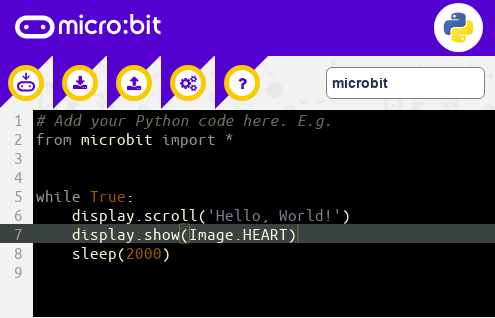
\includegraphics[width=0.65\linewidth]{res/mb-prog2.png}
    \legend{Interface de programmation en ligne}
\end{figure}

\subsubsection{Mu : une interface complète}

Comme le dit (en anglais) la page d’accueil de Mu : Mu est un éditeur de code simple pour les programmeurs débutants. Il est développé en Python et fonctionne sur Windows, OSX, Linux et Raspberry Pi.


\begin{figure}[h]
    \centering
    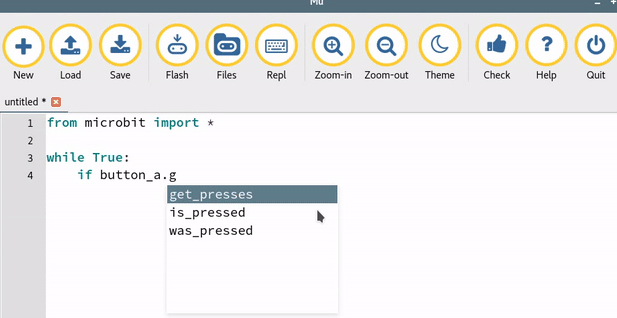
\includegraphics[width=0.65\linewidth]{res/mb-prog3.png}
    \legend{Interface de programmation Mu}
\end{figure}

\subsubsection{Programmation}

L’autocomplétion et l’autoindentation est très efficace. L’interface est rapidement utilisable par un débutant en programmation.
Compilation et enregistrement

Le téléchargement sur la carte se fait très simplement puisqu’il suffit de cliquer sur le bouton Flash . Il est tout de même préférable d’avoir au préalable le réflexe de vérifier le code avec Check .

\subsubsection{Communication série}

La fonction REPL de Mu permet d’ouvrir une communication via un port série avec le \mb. Il est ainsi possible d’envoyer et de recevoir des données. Sur les versions bêta il y a même un plotteur qui permet de visualiser graphiquement les données reçues.

\subsubsection{Documentation}

Il est existe un documentation sur microbit et micropython, qui bien qu’en anglais reste très accessible.

\url{https://microbit-micropython.readthedocs.io/}



%%% Fiches
\newpage\nopagecolor\style{mb}
%\pagestyle{mb}
%\logo{mb}

%   Titre de la sous sections
\section{Borne de satisfaction avec \mb}

%   logo mb ou st dans la table des matières
%\logo{mbot}
%\logo{st}

%
%   style de la page
%   commenter avec % le style non utilisé
 %pour microbit
%\pagestyle{mbot} %pour mbot
%\pagestyle{st} %pour ST

\subsection{Description}

\subsubsection{Objectif}


%   bloc de formule
%   sans titre et fond bleu cyan

\begin{wrapfigure}[3]{r}{5cm}
    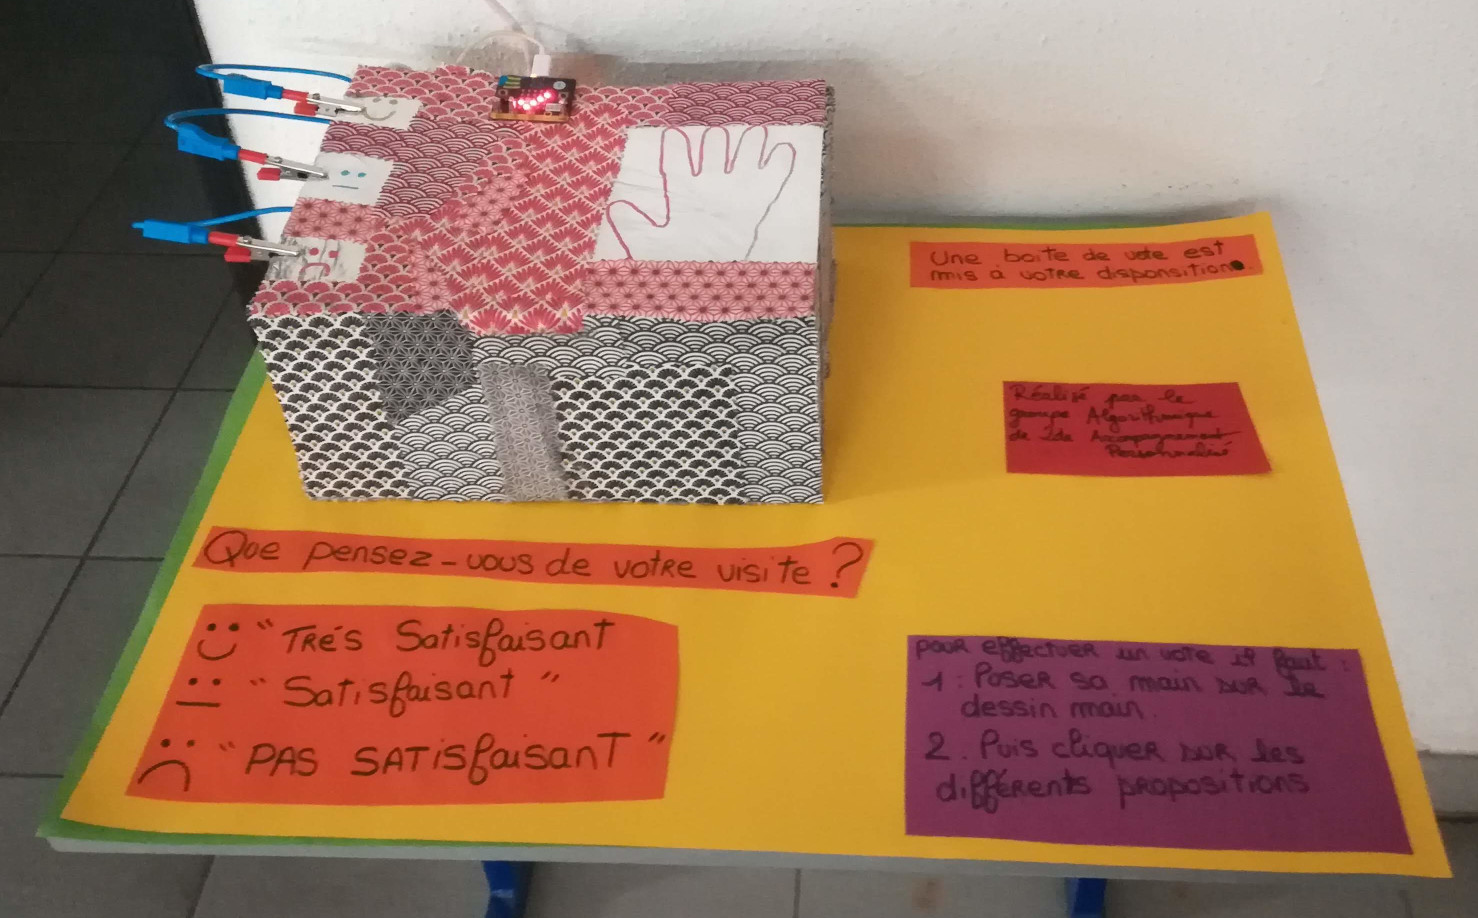
\includegraphics[width=\linewidth]{res/jpo.jpg}
\end{wrapfigure}
    
\begin{formule}
Le but de ce projet est de fabriquer une borne de vote pour un questionnaire de satisfaction. Une question est posée et la réponse est donnée sur une \textbf{échelle de trois valeurs}. Par exemple, la question pourra être \\[1em]

\begin{minipage}[t]{0.7\linewidth}
        \large\textit{\textbf{Journée Portes Ouvertes} : votre avis nous intéresse !\\Que pensez vous de votre visite?} \\[1em]
        \begin{itemize}
            \item {\LARGE\smiley} Très satisfaisant
            \item Satisfaisant
            \item {\LARGE\frownie} Non satisfaisant
        \end{itemize}        
\end{minipage}
    
\end{formule}


\subsubsection{Intérêt}

La borne de satisfaction a été présentée et utilisée lors des journées portes ouvertes, dans nos lycées.

%liste d'arguments
\begin{description}
    \item [Projet concret] Les élèves visualisent rapidement le but à atteindre. Ils ont tous déjà vu une borne de satisfaction et ils imaginent rapidement son utilité. 
    \item [Motivation] La \textit{journée portes ouvertes} est l'occasion de représenter le lycée auprès de personnes extérieures. Les élèves sont fiers de montrer leurs créations.
    \item [Pluridisciplinarité] La création de la borne de satisfaction peut mobiliser de nombreuses disciplines sur le lycée : maths/sciences pour la conduite du projet, mathématiques pour l'exploitation des résultats, mode-vêtement et maroquinerie pour la décoration, arts appliqués pour les visuels ou encore bois, plasturgie et métallurgie pour la boite.
\end{description}


\subsubsection{Matériel}
\begin{itemize}
%   matériel pour micro:bit
    \item 1 $\times$ \matosMb
    \item 1 $\times$ accès internet : IDE programmation par bloc \url{http://makecode.microbit.org/}\\[1em]
    \item 1 boite (carton, bois, métal, etc.)
    \item 4 câbles électriques + 4 pinces crocodiles
    \item 1 rouleau de papier aluminium
\end{itemize}


%
% activité de niveau 
%

%   saut de page
\newpage

%   titre de la sous section
\subsection{Niveau initiation - Premier modèle}

\subsubsection{Activité élève}

% commande perso \CARTOUCHE
%   5 paramètres : 
%       * durée
%       * public
%       * travail en maths
%       * travail en sciences
%       * travail en algo
\cartouche
{1 h}         %durée
{2de}           %public
{}        %maths
{}     %sciences
{boucle ; évènement}       %algo


%   petite image de logo qui va
%   se mettre dans le bloc élève
\begin{wrapfigure}[4]{r}{3cm}
    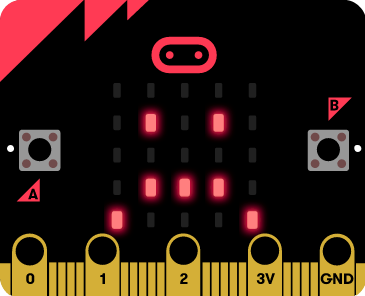
\includegraphics[width=\linewidth]{res/mb_smiley03.png}
\end{wrapfigure}

%   bloc élève
%   fond orange
\begin{eleve}
    La \textit{Journée Portes Ouvertes} aura lieu dans \textbf{1 mois} !\\
    Nous souhaitons créer une borne de satisfaction.
    \begin{center}
        
\includegraphics[width=0.35\linewidth]{res/vote.png}
    \end{center}
    
    \vspace{1em}
    \texttt{\textsc{Ta Mission} : Programme \mb pour simuler une borne de vote.}
    \vspace{1em}
    
    Ta mission doit respecter les contraintes suivantes :
    \begin{description}
        \item[lorsque le bouton A est pressé] une animation de type \textbf{non satisfaisant} apparaît
        \item[lorsque le bouton B est pressé] une animation de type \textbf{très satisfaisant} apparaît
        \item[après chaque animation] afficher un petit mot de remerciement
    \end{description}
\end{eleve}

\newpage

\subsubsection{Notes pour l'enseignant}

%
%   méthode et remarque
%
\begin{methode}
Proposition de résolution :

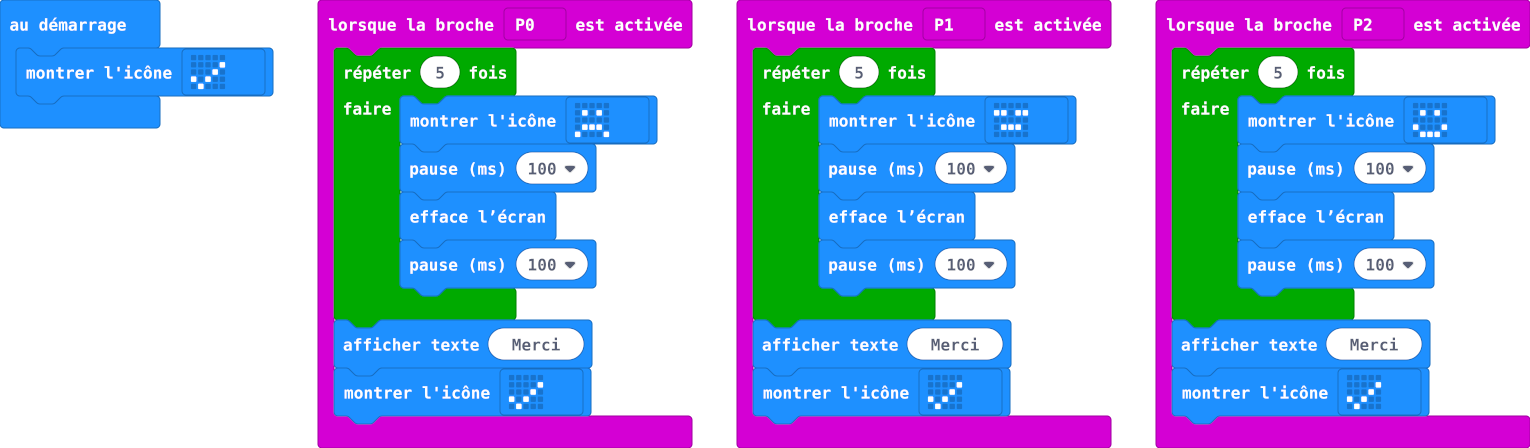
\includegraphics[width=\linewidth]{res/mb-jpo-code01.png}
\end{methode}


\begin{remarque}
    Une proposition de code accessible en ligne
    \url{http://url.univ-irem.fr/w}.
    \begin{center}
        \href {http://url.univ-irem.fr/w}{ 
\includegraphics[scale=0.6]{res/mb-jpo-code01-qr.png}}
    \end{center}
\end{remarque}




\newpage


\subsection{Niveau expert - Cumuler les votes}

\subsubsection{Activité élève}

\cartouche
{1 h}         %durée
{2de}           %public
{effectifs}        %maths
{}     %sciences
{boucle ; évènement ; variables}       %algo


%   petite image de logo qui va
%   se mettre dans le bloc élève
\begin{wrapfigure}[4]{r}{3cm}
    
\includegraphics[width=\linewidth]{res/vote.png}
\end{wrapfigure}

%   bloc élève
%   fond orange
\begin{eleve}
    Bravo ! Tu as réussi à simuler une borne de vote à \textbf{2 choix} : \textit{satisfaisant} ou \textit{non-satisfaisant}.
    
    Notre borne finale sera légèrement différente : 
    \begin{itemize}
        \item la borne aura \textbf{3 choix} de votes possibles : non-satisfaisant ; satisfaisant ; très satisfaisant
        \item la borne \textbf{enregistrera} les réponses de chaque vote.
    \end{itemize}
    
    \vspace{1em}
    \texttt{\textsc{Ta Mission} : (re)Programme \mb pour simuler la borne de vote finale.}
    \vspace{1em}
    
    Modifie ton code précédent :
    \begin{description}
        \item[lorsque la broche p0 est pressée]~\\
            afficher une animation de type \textbf{non satisfaisant}\\
            afficher un mot de remerciement\\
            incrémenter la variable \texttt{\large{n0}}
        \item[lorsque la broche p1 est pressée]~\\
            afficher une animation de type \textbf{satisfaisant}\\
            afficher un mot de remerciement\\
            incrémenter la variable \texttt{\large{n1}}
        \item[lorsque la broche p2 est pressée]~\\
            afficher une animation de type \textbf{très satisfaisant}\\
            afficher un mot de remerciement\\
            incrémenter la variable \texttt{\large{n2}}
        \item[lorsque le bouton A est pressé] afficher les valeurs des variables \texttt{n0}, \texttt{n1} et \texttt{n2}
    \end{description}
\end{eleve}

\newpage

\subsubsection{Notes pour l'enseignant}

%
%   méthode et remarque
%
\begin{methode}
Proposition de résolution :
\begin{center}
    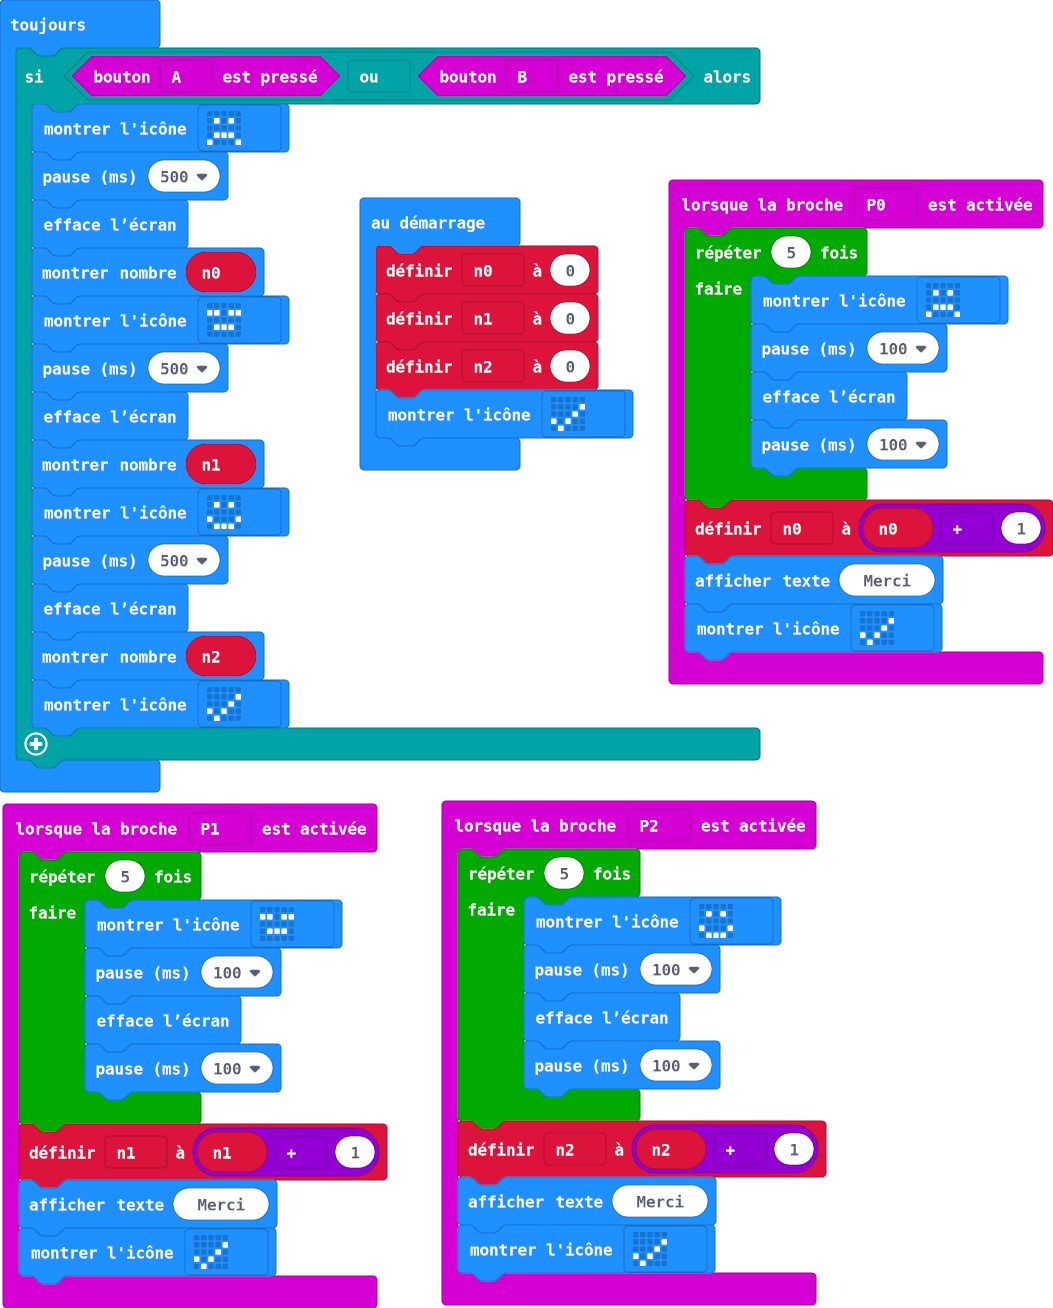
\includegraphics[width=0.75\linewidth]{res/mb-jpo-code02.png}    
\end{center}
\end{methode}


\begin{remarque}
    Une proposition de code accessible en ligne
\url{http://url.univ-irem.fr/y}
    \begin{center}
		\href {http://url.univ-irem.fr/y}
		{
\includegraphics[width=0.2\linewidth]{res/mb-jpo-code02-qr.png}}
    \end{center}
\end{remarque}


\newpage\nopagecolor\section{Les fractions avec \mb}

%   logo mb dans la table des matières
\logo{mb}

% style de page micro:bit
\pagestyle{mb}

\subsection{Description}

\subsubsection{Objectif}

\begin{formule}
Le but de ce projet est :
\begin{description}
    \item [cycle 4] 
        Utiliser diverses représentations d’un même nombre ; passer d’une représentation à une autre.\\
        Comparer, ranger, encadrer des nombres rationnels.
    \item [\textsc{CAP}] 
        Comparer, additionner, soustraire, multiplier et diviser les nombres en écriture fractionnaire dans des situations simples.
\end{description}

\end{formule}

\subsubsection{Intérêt}
Les fractions posent en général des difficultés aux élèves et la majorité font des blocages hérités des années antérieures. Le risque de démobilisation est grand et l'usage d'un objet connecté permet de dédramatiser la séance.

\begin{description}
    \item [Aspect ludique] L'usage de l'affichage LED du micro:bit rend l'activité ludique. Les élèves sont pour la plupart attirés par le côté simple et sympathique de l'écran, ce qui les poussent à réfléchir et s'investir.    
    \item [Proportions] Afficher une image conforme à une contrainte est un problème concret qui permet de mieux matérialiser un calcul de proportion, par rapport à un énoncé classique (type statistiques). En évaluation, il y a plus de réponses justes quand la question repose sur un affichage d'image que sur une situation plus habituelle (point vérifié en classe).
    \item [Plusieurs de méthodes de résolutions] Il y a de nombreuses façons d'arriver aux solutions. Par exemple pour éclairer $\frac{2}{5}$ des LED, on peut d'abord \emph{faire des paquets} de 5, en allumer 2 puis recommencer ; soit éclairer \emph{2 colonnes sur les 5} existantes.
\end{description}


\subsubsection{Matériel}
\begin{itemize}
    \item 1 $\times$ \matosMb \emph{(facultatif car le simulateur peut suffire, même si on perd un peu sur l'aspect ludique.)}
    \item 1 $\times$ accès internet : IDE programmation par bloc \url{http://makecode.microbit.org/}
\end{itemize}



%
% activité de niveau 
%
\newpage
\subsection{Écrire une fraction}
\subsubsection{Activité élève}

% commande perso \CARTOUCHE
%   5 paramètres : 
%       * durée
%       * public
%       * travail en maths
%       * travail en sciences
%       * travail en algo
\cartouche
{0,5 h}
{Cycle 4 ; CAP}
{représentation d'un nombre ; fraction}
{}
{}




%
%   ELEVE
%

\begin{wrapfigure}[1]{r}{1.5cm}
    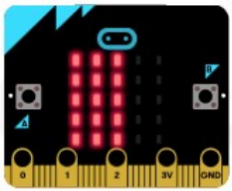
\includegraphics[width=\linewidth]{res/mb-fraction-mini.png}
\end{wrapfigure}




\begin{eleve}    
    \texttt{Écrire la proportion de LED allumée sur chaque micro:bit}
    
    \centerline{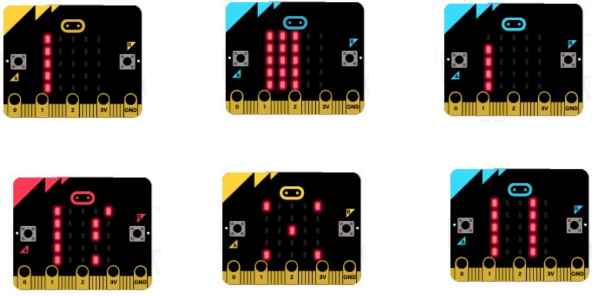
\includegraphics[width=0.75\linewidth]{res/mb-fraction.png}}
\end{eleve}

%
%   PROF
%

\subsubsection{Notes pour l'enseignant}

Attendus:

\begin{itemize}
    \item Les élèves écrivent les fractions correspondant pour chaque appareil.
    \item Lorsque c’est possible, on écrit la fraction sous différentes formes : $\frac {1}{5}$ ou $\frac{5}{25}$.
    \item On écrit alors les conditions d’égalité de deux fractions.
\end{itemize}

\begin{remarque}
    Prolongement  possibles :
    \begin{itemize}
        \item Répondre par une phrase : \emph{il y a 5 LED allumées sur un total de 25}.
        \item Pour chaque cas, indiquer la proportion de LED \emph{éteintes}.
    \end{itemize}
\end{remarque}


%
% activité de niveau 
%
\newpage
\subsection{Afficher une fraction}
\subsubsection{Activité élève}

% commande perso \CARTOUCHE
%   5 paramètres : 
%       * durée
%       * public
%       * travail en maths
%       * travail en sciences
%       * travail en algo
\cartouche{0,5 h}{Cycle 4 ; CAP}{représentation d'un nombre ; fraction}{}{affichage}

%
%   ELEVE
%
\begin{wrapfigure}[4]{r}{3cm}
    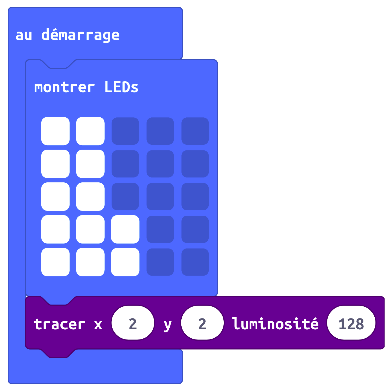
\includegraphics[width=\linewidth]{res/mb-fraction2.png}
\end{wrapfigure}

\begin{eleve}    
    \texttt{Représenter les fractions suivantes avec les LED du micro:bit}
    $$
    \frac{1}{2} \quad ; \quad \frac{32}{100}
    $$
\end{eleve}

%
%   PROF
%
\subsubsection{Notes pour l'enseignant}

Attendus :

\begin{itemize}
    \item Les élèves constatent qu’il n’est pas possible d’afficher un demi, on peut alors leur suggérer d’afficher la 13ème led en alternance ou de lui réduire la luminosité.
    \item Les élèves doivent simplifier la deuxième fraction pour afficher, on peut alors faire le lien avec les pourcentages
\end{itemize}


%
% activité de niveau 
%
\newpage
\subsection{Somme de fractions}
\subsubsection{Activité élève}

% commande perso \CARTOUCHE
%   5 paramètres : 
%       * durée
%       * public
%       * travail en maths
%       * travail en sciences
%       * travail en algo
\cartouche{0,5 h}{Cycle 4 ; CAP}{représentation d'un nombre ; fraction}{}{affichage}

%
%   ELEVE
%
\begin{wrapfigure}[4]{r}{3cm}
    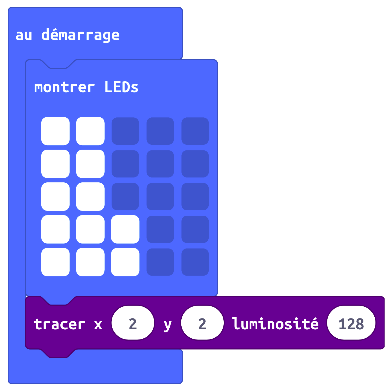
\includegraphics[width=\linewidth]{res/mb-fraction2.png}
\end{wrapfigure}

\begin{eleve}    
    \texttt{Représenter les fractions suivantes avec les LED du \mb :}
    $$
    \frac{2}{5} + \frac{3}{25} \quad ; \quad \frac{23}{25}
    $$
\end{eleve}

%
%   PROF
%
\subsubsection{Notes pour l'enseignant}

\begin{remarque}
Plusieurs raisonnements sont à construire :
\begin{itemize}
    \item créer des paquets de 5 et prendre à chaque fois 2 éléments 
    \item diviser le tout en 5 paquets et en prendre 2
    
\end{itemize}
    
\end{remarque}
\newpage\nopagecolor
\style{mb}


\section{Dé à 6 faces avec \mb}

\subsection{Description}

\subsubsection{Objectif}

\begin{formule}
Le but de ce projet est de simuler une expérience aléatoire de lancer de dé à 6 faces avec une carte \mb.

Toujours à partir d’une situation simple idéale, le programme peut être étoffé au gré des besoins. Il s'agit de prolonger les quelques notions utilisées pour l'activité pile ou face, notamment lorsqu'il faudra tester les différentes issues et proposer une sortie en conséquence.
\end{formule}

\subsubsection{Intérêt}
L'intérêt de cette activité n'est pas seulement de se départir des bruits des dés qui roulent dans la classe; l'usage du \mb est ici très pertinent, tant pour les probabilités que pour la programmation.
\begin{description}
    \item [Simplicité de la situation.] La situation est très simple à expliquer et les élèves comprennent le but à atteindre. L'absence de difficulté mathématique rend cette situation particulièrement simple à mettre en œuvre.
    \item [Motivation des élèves.] L'envie de programmer un objet connecté est grande pour les élèves. Cette façon de programmer, \emph{utile, concrète et appliquée}, leur correspond parfaitement.
    \item [De nombreuses solutions/améliorations possibles.] Comme pour bien des projets, il y a plusieurs façons d'arriver à la solution; mais par rapport à l'activité \emph{Pile ou Face} il y aussi plus de possibilité de faire des erreurs de programmation.
    \item [Travail mathématique sur la modélisation.] La modélisation d'un dé non truqué est évidente, et n'apporte pas de difficulté majeure. Par contre l'intérêt majeur du \mb est d'offrir la possibilité de truquer le dé. On a alors une situation beaucoup plus riche, tant dans la modélisation que dans les usages du modèle obtenu.
\end{description}


\subsubsection{Matériel}
\begin{itemize}
    \item 1 $\times$ \matosMb \emph{(facultatif car le simulateur peut suffire)}
    \item 1 $\times$ accès internet : IDE programmation par bloc \url{http://makecode.microbit.org/}
\end{itemize}


%
% activité de niveau 1
%
\newpage
\subsection{Niveau simple}
\subsubsection{Activité élève}

% commande perso \CARTOUCHE
%   5 paramètres : 
%       * durée
%       * public
%       * travail en maths
%       * travail en sciences
%       * travail en algo
\cartouche{0,25 h}{2de}{expérience aléatoire}{}{affichage ; événement.}

\begin{eleve}

\begin{wrapfigure}[4]{r}{3.5cm}
	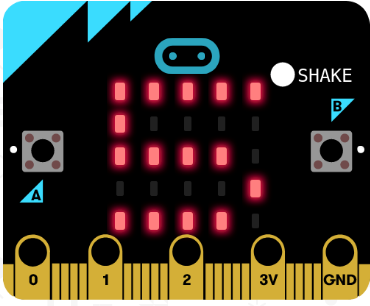
\includegraphics[width=\linewidth]{res/mbDe6FacesN1.png}
\end{wrapfigure}

\texttt{\textsc{Mission} Utilise \mb~pour simuler un \emph{dé à 6 faces} !}


En t'aidant des blocs ci-dessous, programme \mb~pour : 
\begin{enumerate}
    \item programmer un événement lorsque l'appareil est secoué;
    \item afficher \emph{un nombre entier aléatoire} entre \texttt{1} et \texttt{6}.
\end{enumerate}
~\\
\centerline{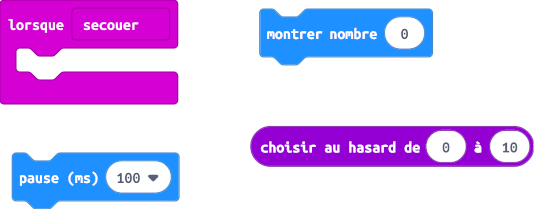
\includegraphics[width=0.6\textwidth]{res/mbDe6FacesN1blocs.png}}

\end{eleve}


\subsubsection{Notes pour l'enseignant}

Ce premier niveau aucun niveau de difficulté, on pourrait dire que son intérêt se limite à poser la problématique.

\begin{minipage}[t]{0.5\linewidth}
    \begin{methode}
    ~\\Pour résoudre ce problème, il suffit de programmer les instructions de la façon suivante :
    
    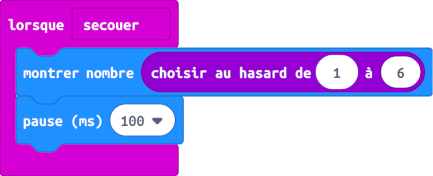
\includegraphics[width=0.4\linewidth]{res/mbDe6FacesN1proposition.png}
    \end{methode}
\end{minipage}
\hfill
\begin{minipage}[t]{0.5\linewidth}
    \begin{remarque}
    ~\\Plus d'informations sur la page de l'activité :\\ \url{https://microbit.readthedocs.io/fr/latest/decouverte/de6faces-bloc1.html}
    \end{remarque}
\end{minipage}






%
% activité de niveau 2
%
\newpage
\subsection{Niveau intermédiaire}
\subsubsection{Activité élève}

% commande perso \CARTOUCHE
%   5 paramètres : 
%       * durée
%       * public
%       * travail en maths
%       * travail en sciences
%       * travail en algo
\cartouche{0,5 h}{2de}{expérience aléatoire}{}{affichage ; événement ; condition}


\begin{eleve}
	
	
\begin{wrapfigure}[7]{r}{4cm}
	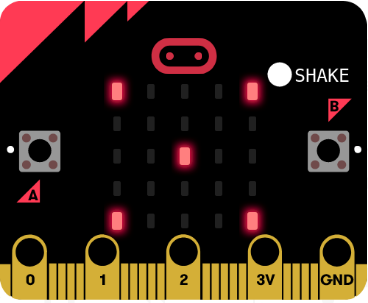
\includegraphics[width=\linewidth]{res/mbDe6FacesN2.png}
\end{wrapfigure}

Utilise \mb~pour simuler un \emph{dé à 6 faces} !

En t'aidant des blocs ci-dessous, programme \mb~pour : 
\begin{enumerate}
    \item programmer un événement lorsque l'appareil est secoué;
    \item afficher \emph{une face de dé} selon le résultat d'un tirage aléatoire.
\end{enumerate}
Attention tous les blocs ne sont pas représentés et certains blocs doivent être modifiés.

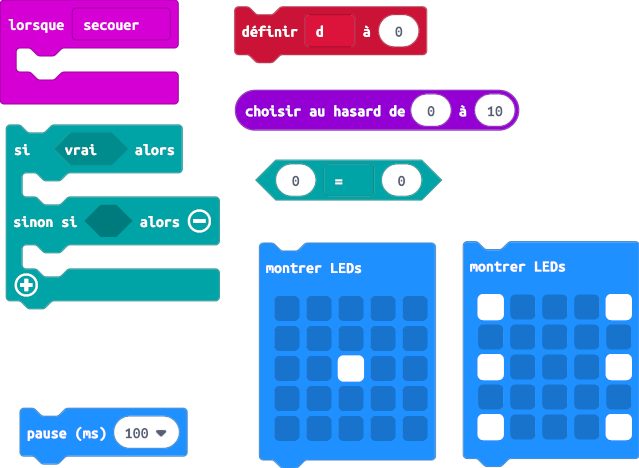
\includegraphics[width=0.6\textwidth]{res/mbDe6FacesN2blocs.png}

\end{eleve}

\newpage
\subsubsection{Notes pour l'enseignant}

Pour arriver au résultat escompté il est nécessaire d'utiliser une variable, ainsi qu'une suite d'instruction si/sinon si/sinon. Si l'usage d'une variable n'apparaît pas forcément évident pour les élèves, on peut les laisser programmer sans pour qu'il puisse ainsi constater le bug produit.
Il est aussi intéressant de faire remarquer aux élèves que le nombre issue du tirage aléatoire n'a pas forcément à être celui symbolisé par sortie sur l'écran de DEL.


\begin{minipage}[t]{0.5\linewidth}
    \begin{methode}~\\
    Pour résoudre ce problème, il suffit de programmer les instructions de la façon suivante (seules les sorties correspondant à 1 et à 6 ont été incluses, pour raison de place) :
    
    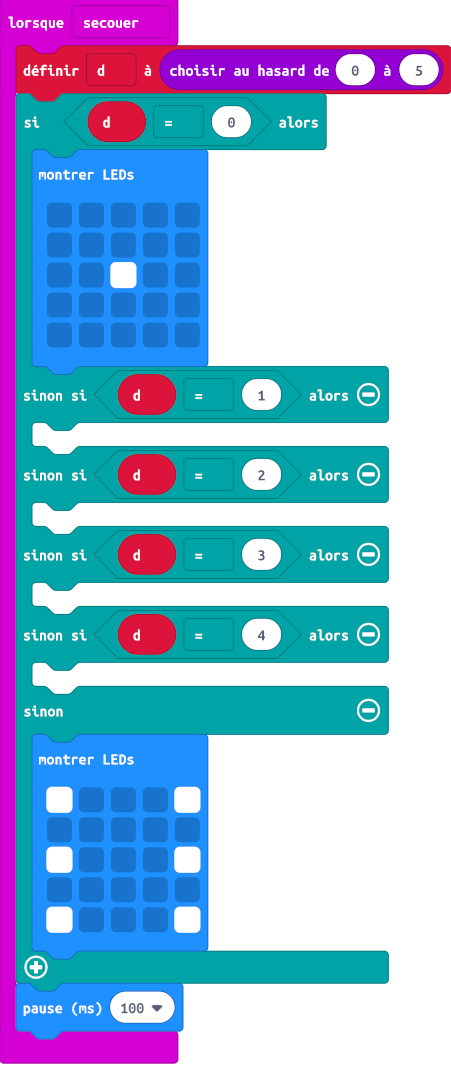
\includegraphics[width=0.85\linewidth]{res/mbDe6FacesN2propos.png}
    \end{methode}
\end{minipage}
\hfill
\begin{minipage}[t]{0.5\linewidth}
    \begin{remarque}~\\
    Il est très simple en partant de cette situation d'envoyer les résultats par radio ver un \mb qui centraliserait alors les issues de l'ensemble des tirages. Pour cela il suffit d'ajouter le bloc "envoyer le nombre" qui se trouve dans la catégorie "Radio".
    
    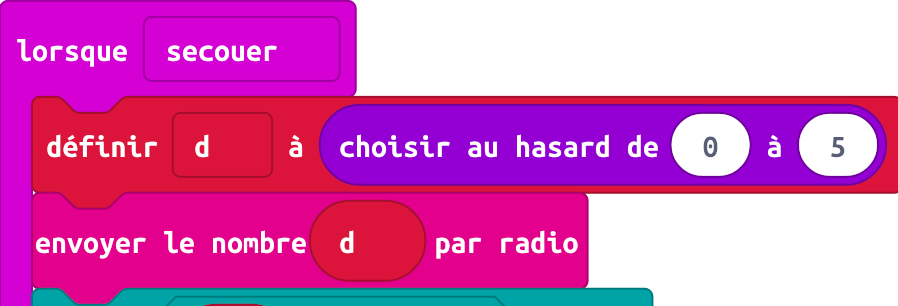
\includegraphics[width=\linewidth]{res/mbDe6FacesN2radio.png}
    
    Plus d'informations sur la page de l'activité :\\ \url{https://microbit.readthedocs.io/fr/latest/decouverte/de6faces-bloc2.html}
    \end{remarque}
\end{minipage}
\newpage\nopagecolor\style{mb} %pour microbit


%   Titre de la sous sections
\section{Normal ou truqué? avec \mb}
%   logo mb dans la table des matières
%\logo{mb}

%
%   style de la page
%   commenter avec % le style non utilisé
%\pagestyle{st} %pour ST

\subsection{Description}

\subsubsection{Objectif}


%   bloc de formule
%   sans titre et fond bleu cyan
\begin{formule}
Cette activité propose à l'élève de travailler sur la \emph{fluctuation d'échantillonnage}.

Sans accéder au code, seulement \emph{en manipulant} la carte \mb, l'élève doit déterminer si le jeu téléversé est un jeu \emph{normal} ou \emph{truqué}\ldots
\end{formule}


\subsubsection{Intérêt}

L'intérêt de cette activité est de pouvoir, en toute liberté, créer des situations équiprobables ou non. Même s'il est possible d'utiliser de vrais dès truqués, l'utilisation d'une carte \mb permet un éventail très larges de situations.

Ici le choix a été fait de procéder à un tirage aléatoire (ou non ;) ) d'un nombre entre 0 et 9 (inclus).


\subsubsection{Matériel}
\begin{itemize}
%   matériel pour micro:bit
    \item 1 $\times$ \matosMb \emph{(facultatif car le simulateur peut suffire)}
%   site pour micro:bit
    \item 1 $\times$ accès internet : IDE programmation par bloc \url{http://makecode.microbit.org/}
\end{itemize}



\subsubsection{Progression}

L'activité se déroule en 2 temps :
\begin{description}
    \item[Analyse du programme] Dans cette partie, l'élève doit étudier les deux programmes possibles (truqué ou non) puis répondre à une série de questions de probabilités
    \item[Expérience aléatoire] Ensuite l'élève manipule la carte \mb et effectue un certain nombre d'expériences aléatoires. Dans cette partie l'analyse des échantillons et la création d'une représentation graphique permettra de conclure sur le type de programme téléversé.
\end{description}

%
% activité de niveau 
%

%   saut de page
\newpage

%   titre de la sous section
\subsection{Activité}

\subsubsection{Activité élève}

% commande perso \CARTOUCHE
%   5 paramètres : 
%       * durée
%       * public
%       * travail en maths
%       * travail en sciences
%       * travail en algo
\cartouche
{2 h}         %durée
{2de ; term}           %public
{fluctuation d'échantillage}        %maths
{}     %sciences
{}       %algo


%   petite image de logo qui va
%   se mettre dans le bloc élève
\begin{wrapfigure}[4]{r}{2cm}\rule{0cm}{2pt}
    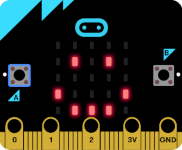
\includegraphics[width=\linewidth]{res/mb-truque-mini.png}
\end{wrapfigure}

%   bloc élève
%   fond orange
\begin{eleve}    
    \texttt{\textsc{Normal ou \emph{truqué} ?}}
    
    Sur votre carte est téléversé un des deux programmes de jeu suivant. Quand le joueur gagne, il a un smiley sourire, sinon il a  une croix. 
    
    
    
%   ajout d'une image
\begin{minipage}[t]{0.5\linewidth}
    \begin{center}
        \vspace{0cm}
        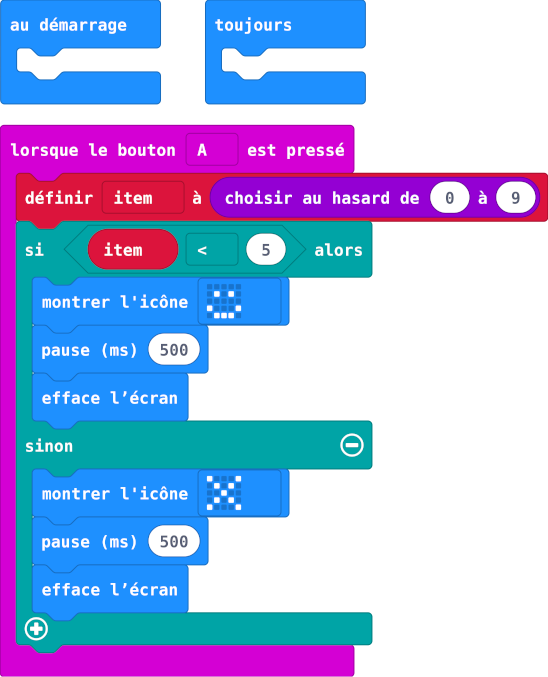
\includegraphics[width=0.7\linewidth]{res/mb-normal.png}\\
        Jeu \emph{normal}
    \end{center}
\end{minipage}
\hfill
\begin{minipage}[t]{0.5\linewidth}
    \begin{center}
        \vspace{0cm}
        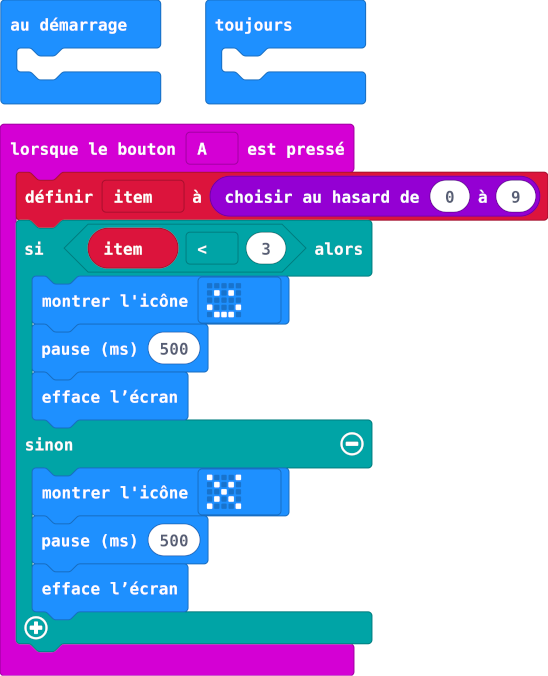
\includegraphics[width=0.7\linewidth]{res/mb-truque.png}\\
        Jeu \emph{truqué}
    \end{center}
\end{minipage}
    
    \textbf{Analyse du programme}
    
    \begin{enumerate}
        \item   Si on choisit un nombre entier au hasard entre 0 et 9, combien y-a-t-il d’issues possibles ?
        \item Si pour gagner il faut obtenir un nombre entre 0 et 4, combien y-a-t-il d’issues favorables ?  
        \item Calculer la probabilité de gagner avec la version normale du programme. Donner le résultat sous forme de fraction, de nombre décimal et de pourcentage.
        \item Avec le même raisonnement, calculer la probabilité de gagner avec la version truquée du programme. Donner le résultat sous forme de fraction, de nombre décimal et de pourcentage.
    \end{enumerate}
    
    \newpage
    \textbf{Analyse du programme}
    
    \begin{enumerate}
        \setcounter{enumi}{4}
        \item \emph{Jouer des parties} par séquence de 25 parties et noter G pour gagner et P pour perdu, dans votre cahier.
        \item En utilisant vos résultats, compléter le tableau ci-dessous. \emph{Attention !} Bien prendre son temps pour compter.\\
        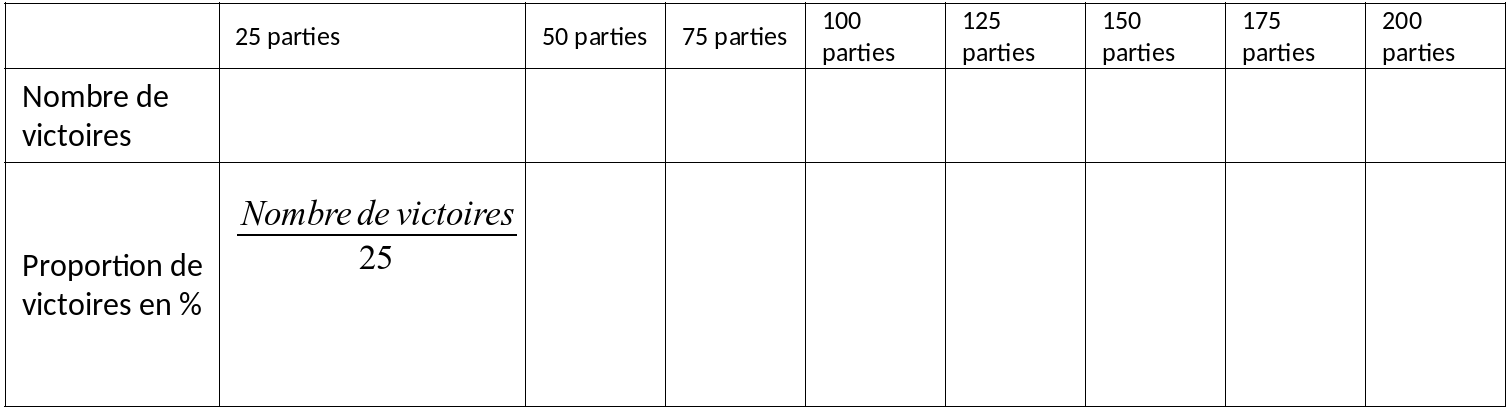
\includegraphics[width=\linewidth]{res/mb-truque-activite2.png}
        \item Compléter le graphique correspondant à la dernière ligne du tableau : placer un point par colonne, relier les points par des segments et légender les axes.\\
        Donner un \emph{titre} au graphique.\\
          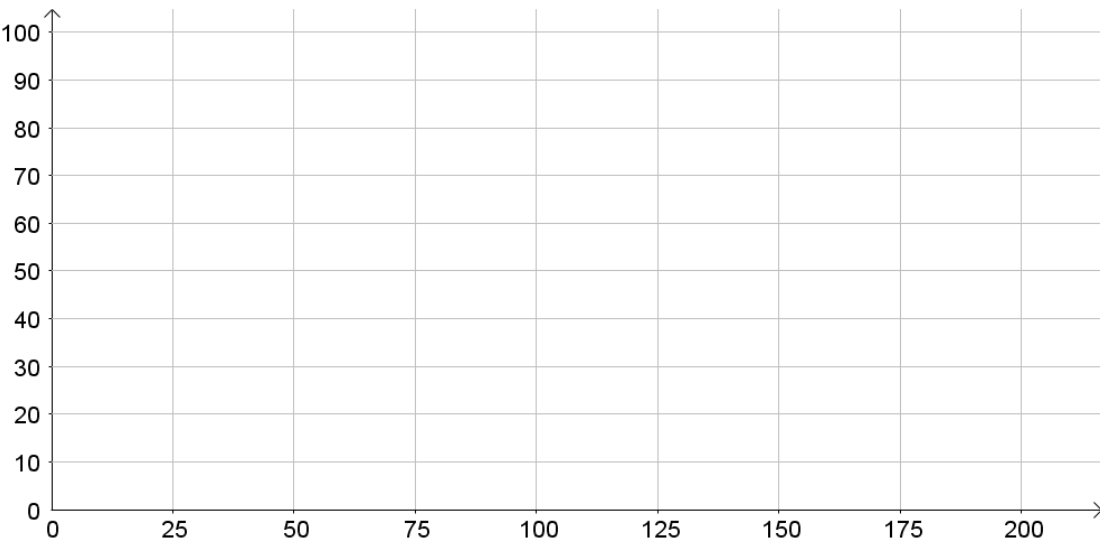
\includegraphics[width=\linewidth]{res/mb-truque-activite3.png}
        \item Analyser le graphique et conclure sur le programme qui est téléchargé dans votre carte.\\
        Argumenter avec une ou plusieurs phrases.
    \end{enumerate}
    
\end{eleve}



\subsubsection{Notes pour l'enseignant}

\begin{remarque}
    Le code \emph{interactif} est accessible en ligne : 
    \begin{description}
        \item[Jeu normal] \url{https://makecode.microbit.org/_0E1iAAee46YC}
        \item[Jeu truqué] \url{https://makecode.microbit.org/_4zFAsTUuEgYV}
    \end{description}
\end{remarque}
\newpage\nopagecolor\section{Pile ou face avec \mb}

%   logo mb dans la table des matières
\logo{mb}

% style de page micro:bit
\pagestyle{mb}

\subsection{Description}

\subsubsection{Objectif}

\begin{formule}
Le but de ce projet est de simuler une expérience aléatoire de lancer de pièce avec une carte \mb.

À partir d’une situation simple, idéale pour une prise en main de l’interface de programmation, il s’agit par la suite d’améliorer le programme pas à pas. L’objectif est d’obtenir un programme utilisable dans le cadre d’un cours sur les statistiques et les probabilités.
\end{formule}

\subsubsection{Intérêt}
Bien évidemment, travailler avec une carte \mb n'exclut pas de réaliser des expériences aléatoires réelles (pièces, dés, etc.). Cependant, il est très intéressant pour l'enseignant d'utiliser des \mb dans cette partie du programme.
\begin{description}
    \item [Simplicité de la situation.] La situation est très simple à expliquer et les élèves comprennent le but à atteindre. L'absence de difficulté mathématique rend cette situation particulièrement simple à mettre en œuvre.
    \item [Motivation des élèves.] L'envie de programmer un objet connecté est grande pour les élèves. Cette façon de programmer, \emph{utile, concrète et appliquée}, leur correspond parfaitement.
    \item [De nombreuses solutions/améliorations possibles.] Comme pour bien des projets, il y a plusieurs façons d'arriver à la solution. Par ailleurs, les élèves peuvent apporter ou proposer de nombreuses améliorations. La programmation par bloc, exempte de difficulté syntaxique, est particulièrement adaptée à la créativité.
    \item [Travail mathématique sur la modélisation.] Cette compétence n'est pas facile à mettre en œuvre. Ici, l'absence de difficultés mathématiques rend ce travail beaucoup plus accessible à tous.
\end{description}


\subsubsection{Matériel}
\begin{itemize}
    \item 1 $\times$ \matosMb \emph{(facultatif car le simulateur peut suffire)}
    \item 1 $\times$ accès internet : IDE programmation par bloc \url{http://makecode.microbit.org/}
\end{itemize}



%
% activité de niveau 1
%
\newpage
\subsection{Niveau simple}
\subsubsection{Activité élève}

% commande perso \CARTOUCHE
%   5 paramètres : 
%       * durée
%       * public
%       * travail en maths
%       * travail en sciences
%       * travail en algo
\cartouche{0,5 h}{2de}{expérience aléatoire}{}{affichage ; boucle ; événement.}



\begin{wrapfigure}[4]{r}{3.5cm}
    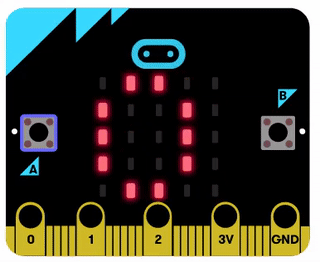
\includegraphics[width=\linewidth]{res/mbPileFaceN1.png}
\end{wrapfigure}
\begin{eleve}
\texttt{\scshape{Mission : }
Utilise \mb~pour jouer à \emph{Pile ou Face} !}

En t'aidant des blocs ci-dessous, programme \mb~pour : 
\begin{enumerate}
    \item afficher une courte animation ;
    \item afficher \emph{de façon aléatoire} \texttt{0} ou \texttt{1}.
\end{enumerate}

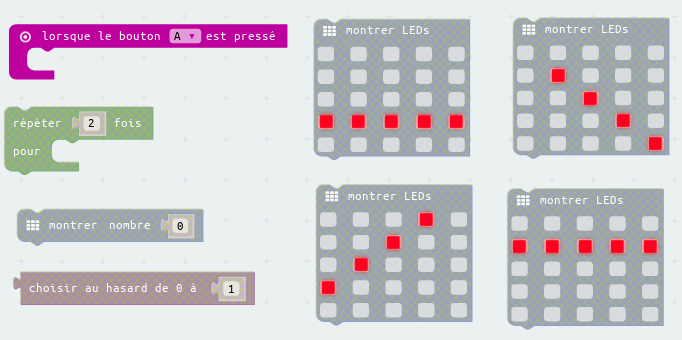
\includegraphics[width=\textwidth]{res/mbPileFaceN1blocs}

\end{eleve}


\newpage
\subsubsection{Notes pour l'enseignant}

Ce premier niveau permet de se familiariser avec l’interface tout en produisant un premier programme fonctionnel et utile.

\begin{minipage}[t]{0.5\linewidth}
    \begin{methode}~\\
    Pour résoudre ce problème, il suffit de programmer les instructions de la façon suivante :
    
    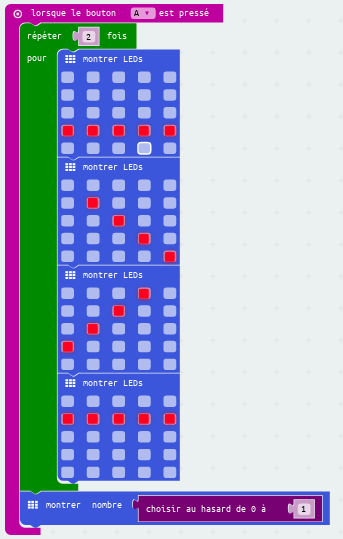
\includegraphics[width=\linewidth]{mbPilefaceN1proposition}
    \end{methode}
\end{minipage}
\hfill
\begin{minipage}[t]{0.5\linewidth}
    \begin{remarque}~\\
    Plus d'informations sur la page de l'activité :\\ \url{https://microbit.readthedocs.io/fr/latest/decouverte/pileface-bloc1.html}
    \end{remarque}
\end{minipage}









%
% activité de niveau 2
%
\newpage
\subsection{Niveau intermédiaire}
\subsubsection{Activité élève}

% commande perso \CARTOUCHE
%   5 paramètres : 
%       * durée
%       * public
%       * travail en maths
%       * travail en sciences
%       * travail en algo
\cartouche{0,5 h}{2de}{expérience aléatoire}{}{affichage ; boucle ; événement ; condition ; fonction.}


\begin{wrapfigure}[4]{r}{3.5cm}
    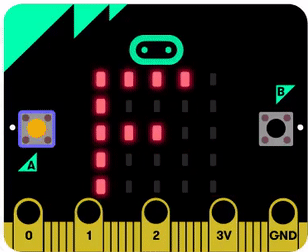
\includegraphics[width=\linewidth]{res/mbPileFaceN2.png}
\end{wrapfigure}
\begin{eleve}
Maintenant, {\Large{améliore}} le programme de ton \mb.

Voici deux idées :
\begin{itemize}
    \item au lieu d'afficher \texttt{0} ou \texttt{1}, affiche plutôt \texttt{P} ou \texttt{F} ;
    \item utilise une fonction pour gérer ton animation.
\end{itemize}
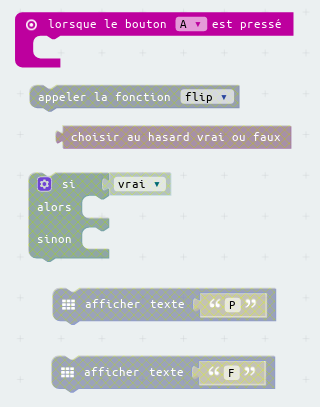
\includegraphics[width=0.5\textwidth]{res/mbPilefaceN2blocs.png}
\end{eleve}


\newpage
\subsubsection{Notes pour l'enseignant}

Ce deuxième niveau est l'occasion d'introduire les notions de fonctions et les branchements conditionnels.

\begin{methode}
Voici une proposition qui fonctionne :

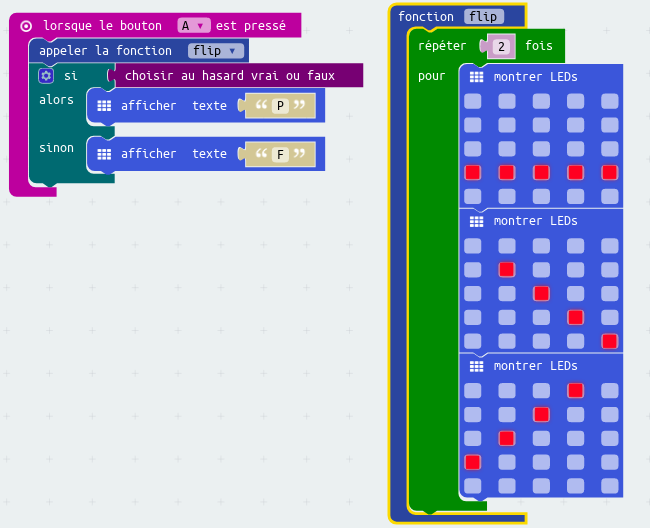
\includegraphics[width=\linewidth]{res/mbPilefaceN2proposition.png}
\end{methode}

\begin{remarque}
Plus d'informations sur la page de l'activité :\\ \url{https://microbit.readthedocs.io/fr/latest/decouverte/pileface-bloc2.html}
\end{remarque}





%
% activité de niveau 3
%
\newpage
\subsection{Niveau expert}
\subsubsection{Activité élève}

% commande perso \CARTOUCHE
%   5 paramètres : 
%       * durée
%       * public
%       * travail en maths
%       * travail en sciences
%       * travail en algo
\cartouche{0,5 h}{2de}{expérience aléatoire}{}{affichage ; boucle ; événement ; condition ; fonction ; variable (incément) ; texte (concaténation).}


\begin{wrapfigure}[4]{r}{2.5cm}
    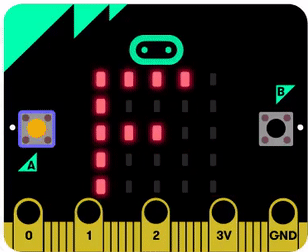
\includegraphics[width=\linewidth]{res/mbPileFaceN2.png}
\end{wrapfigure}
\begin{eleve}
Est ce que \mb peut afficher les tirages obtenus ?

Pour finir, nous souhaitons ajouter une fonctionnalité supplémentaire à \mb. Il faut maintenant arriver à afficher l'effectif total pour les \texttt{Piles} et pour les \texttt{Faces}.

Regarde ci-dessous les instructions que tu pourrais ajouter.

\centerline{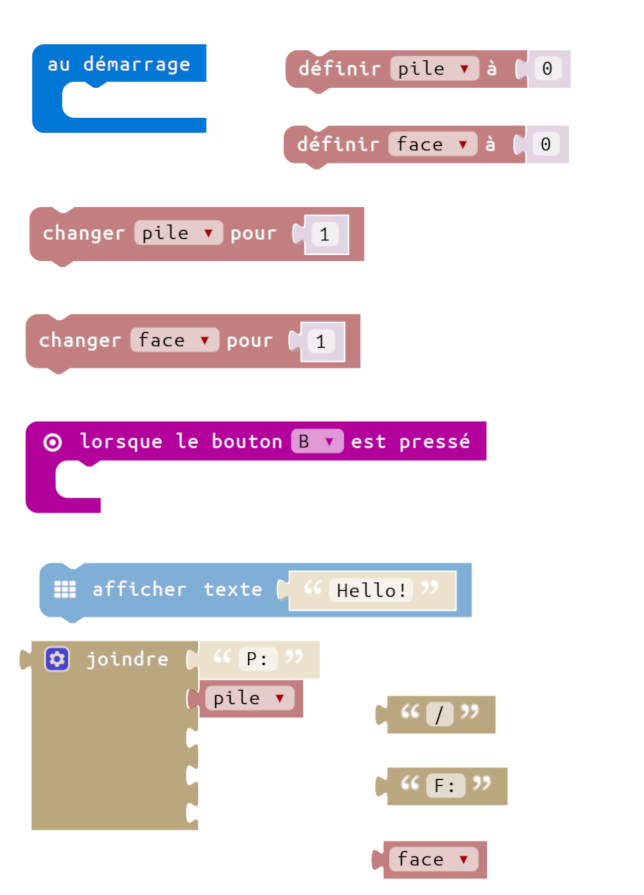
\includegraphics[width=0.4\textwidth]{mbPilefaceN3blocs.png}}
\end{eleve}



\newpage
\subsubsection{Notes pour l'enseignant}

Dans ce troisième niveau, nous souhaitons compter les issues obtenues et afficher les totaux. Il faut introduire la notion de variable informatique.

\begin{methode}
Le résultat escompté est le suivant :\\
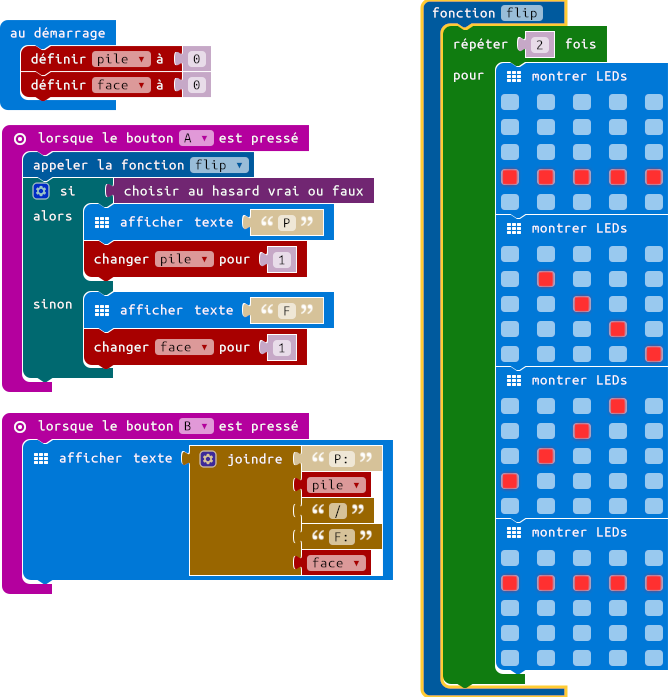
\includegraphics[width=\linewidth]{res/mbPilefaceN3proposition.png}
\end{methode}

\begin{remarque}
Plus d'informations sur la page de l'activité :\\ \url{https://microbit.readthedocs.io/fr/latest/decouverte/pileface-bloc3.html}
\end{remarque}



\newpage\nopagecolor\section{Fluctuation d'échantillonnage avec \mb}

%   logo mb ou st dans la table des matières
\logo{mb}
%\logo{mbot}
%\logo{st}

%
%   style de la page
%   commenter avec % le style non utilisé
\pagestyle{mb} %pour microbit
%\pagestyle{mbot} %pour mbot
%\pagestyle{st} %pour ST

\subsection{Description}

\subsubsection{Objectif}


%   bloc de formule
%   sans titre et fond bleu cyan
\begin{formule}
Le but de ce projet est d'expérimenter la fluctuation d'échantillonnage à  partir d'une situation classique, en établissant tout d'abord un modèle d'expérience aléatoire à partir des données de la situation, puis en proposant de programmer le tirage d'échantillons pour une taille n fixée.
\end{formule}


\subsubsection{Intérêt}

 L'utilisation de l'interface \mb permet d'obtenir rapidement un programme fonctionnel, mais aussi d'afficher graphiquement la série de données produites par le simulateur. Cela représente un intérêt non-négligeable lorsque l'on souhaite traiter la fluctuation d'échantillonnage.

%liste d'arguments
\begin{description}
    \item [Simulation d'une grande série d'expériences aléatoires] Contrairement à l'usage du tableur, où l'élève va devoir manipuler un grand nombre de données en colonnes et en lignes, au risque de se perdre dans leur traitement, l'approche algorithmique de  ce problème permet d'aller à l'essentiel.
    \item [Afficher les données]
    L'utilisation de l'interface \mb permet d'obtenir rapidement un programme fonctionnel, mais aussi d'afficher graphiquement la série de données produites par le simulateur. Cela représente un intérêt non-négligeable lorsque l'on souhaite traiter la fluctuation d'échantillonnage.
\end{description}


\subsubsection{Matériel}
\begin{itemize}
%   matériel pour micro:bit
    \item 1 $\times$ \matosMb \emph{(facultatif car le simulateur peut suffire)}
%   site pour micro:bit
    \item 1 $\times$ accès internet : IDE programmation par bloc \url{http://makecode.microbit.org/}
    \item lien vers l'activité 1 : \url{https://makecode.microbit.org/_TbPFTK8eaKes}
    \item lien vers l'activité 2 : \url{https://makecode.microbit.org/_PW8LCg82z3fh}
    \item lien vers l'activité 3 :
    \url{https://makecode.microbit.org/_11aUTkWzR60J}
\end{itemize}

\newpage

\subsubsection{Progression proposée}


%   bloc méthode
%   titre + fond bleu
\begin{methode}
    On propose ici d'aborder la problématique en trois temps :
    
    \begin{enumerate}
        \item \textbf{Prise en main - Vérifier le modèle.} \\
            Pour faciliter la prise en main et gagner du temps on propose aux élèves de vérifier un code déjà prêt. Cela facilite l'appropriation du problème.
        \item \textbf{Intermédiaire - Du modèle à la génération d'échantillons.}\\
            À partir du modèle, l'élève doit élaborer un algorithme afin de produire des échantillons de taille fixé.
        \item \textbf{Avancé - Visualisation des données}\\
            Cette étape consiste en une amélioration du programme précédent afin de pouvoir visualiser les données issues de la simulation.
            
    \end{enumerate}
\end{methode}

%
% activité de niveau 1
%

%   saut de page
\newpage

%   titre de la sous section
\subsection{Niveau prise en main - Vérifier le modèle\ldots}

\subsubsection{Activité élève}

% commande perso \CARTOUCHE
%   5 paramètres : 
%       * durée
%       * public
%       * travail en maths
%       * travail en sciences
%       * travail en algo
\cartouche
{0,3 h}         %durée
{première}           %public
{statistiques et probabilités}        %maths
{}     %sciences
{instruction conditionnelle}       %algo


%   petite image de logo qui va
%   se mettre dans le bloc élève
\begin{wrapfigure}{r}{3cm}
    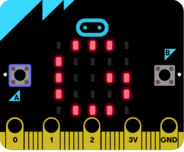
\includegraphics[width=\linewidth]{res/mb-fluctuations-illustration.png}
\end{wrapfigure}

%   bloc élève
%   fond orange
\begin{eleve}    
    \texttt{\textsc{Ta Mission} : Utiliser \mb pour simuler des \emph{naissances}!}
    
    La situation est la suivante : à Ufa, en Russie, 51,2 \%  des naissances sont des garçons.
    
    Dans cette ville, une usine agrochimique expose ses employés à des pesticides contenant de la dioxine.
    
    D’après une étude de l’université de Montréal, parmi les 227 enfants nés d’un parent travaillant dans cette usine, 91 sont des garçons.
    
    Cette étude cherche à déterminer si l’usine interfère sur les naissances.
    
    Pour simuler les naissances à Ufa, on propose d'utiliser le programme ci-dessous.
    
    \emph{Expliquer pourquoi} ce programme modélise correctement les naissance à Ufa.
    
    \emph{Proposer} une façon de l'exploiter afin de vérifier l'influence des produits chimiques sur les naissances.
    
%   ajout d'une image
    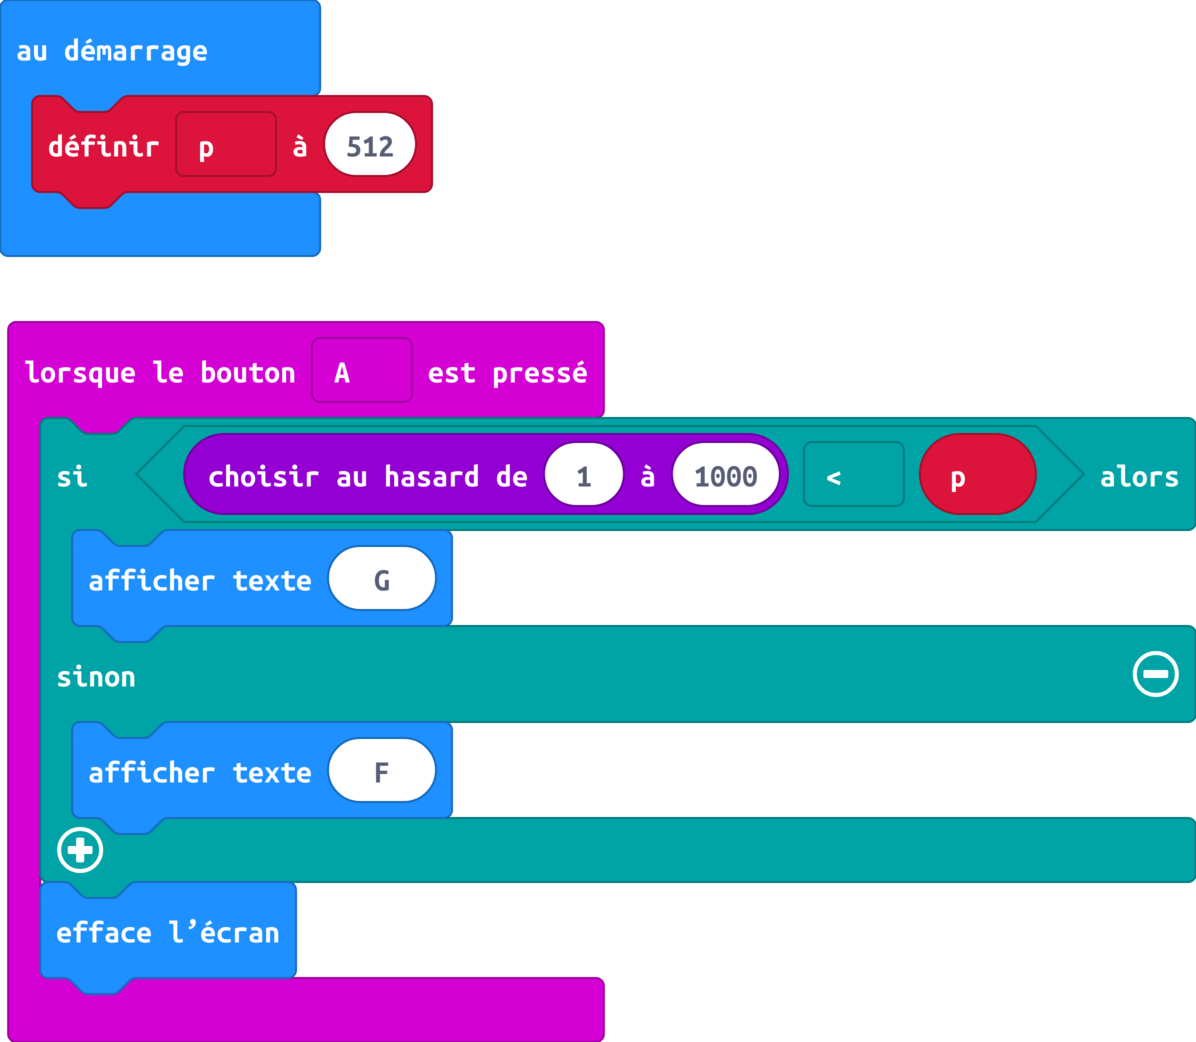
\includegraphics[width=0.5\linewidth]{res/mb-fluctuation-activite1.png}
    
\end{eleve}



\subsubsection{Notes pour l'enseignant}

%
%   méthode et remarque
%
\begin{methode}
Dans cette activité, il s'agit de vérifier que les élèves ont bien compris la problématique et notamment comment est utilisé la fréquence d'apparition du caractère "garçon".

Bien entendu il faut suggérer aux élèves de tester le programme, afin d'en appréhender les limites.
\end{methode}


\begin{remarque}
    Ici l'utilisation de la variable \emph{p} n'est pas indispensable pour l'algorithme. Son intérêt est pédagogique : elle permet de mettre en évidence la donnée utilisée ainsi que de de faire le lien avec le vocabulaire et les notations utilisées dans le cours.

   Avant de passer à l'activité 2, il peut être préférable de lister avec les élèves les éléments manquants qui permettraient de produire et de traiter un échantillon comparable à celui de l'étude :
   \begin{itemize}
       \item une boucle répéter afin de produire un échantillon de taille 227
       \item des variables pour dénombrer les naissances de garçons (et de filles ?)
   \end{itemize}
\end{remarque}

%
% activité de niveau 2
%

%   saut de page
\newpage

%   titre de la sous section
\subsection{Niveau intermédiaire - Générer des échantillons\ldots}

\subsubsection{Activité élève}

% commande perso \CARTOUCHE
%   5 paramètres : 
%       * durée
%       * public
%       * travail en maths
%       * travail en sciences
%       * travail en algo
\cartouche
{0,5 h}         %durée
{première}           %public
{statistiques et probabilités}        %maths
{}     %sciences
{instruction conditionnelle; boucle}       %algo


%   petite image de logo qui va
%   se mettre dans le bloc élève
\begin{wrapfigure}{r}{3cm}
    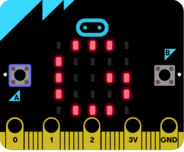
\includegraphics[width=\linewidth]{res/mb-fluctuations-illustration.png}
\end{wrapfigure}

%   bloc élève
%   fond orange
\begin{eleve}    
    \texttt{\textsc{Ta Mission} : Utiliser \mb pour simuler des \emph{naissances}!}
    
    Utilise les blocs proposés afin de générer des échantillons de taille identique à celui de l'étude.
    
    \emph{Construire} un programme qui affiche le nombre de garçons obtenus dans un échantillons de 227 naissances.
    
    \emph{Utiliser} le programme afin de vérifier si la situation de la problématique est vraisemblable.
    
%   ajout d'une image
    \includegraphics[width=0.8\linewidth]{res/mb-fluctuation-activite2-blocs.png}
    
\end{eleve}

%   saut de page
\newpage

\subsubsection{Notes pour l'enseignant}

%
%   méthode et remarque
%
\begin{methode}
Dans cette activité, il s'agit de vérifier que les élèves se sont bien appropriés la problématique, notamment par rapport à la taille de l'échantillon.

Bien entendu il faut suggérer aux élèves de tester le programme plusieurs fois.

Le programme attendu peut être celui-ci si l'élève a utilisé tous les blocs proposés (voir \emph{Remarque} ci-dessous) :

%   ajout d'une image
    \includegraphics[width=0.8\linewidth]{res/mb-fluctuation-activite2-proposition.png}

\end{methode}


\begin{remarque}
    Ici l'utilisation de la variable \emph{f} n'est pas indispensable pour l'algorithme. Son intérêt est pédagogique : elle permet de faire le lien avec l'activité précédente en conservant le modèle proposé.

   Avant de passer à l'activité 3, il est tout de même préférable de faire s'interroger les élèves sur la nécessité de l'existence de la variable \emph{f}.
   
   Enfin, on interrogera les élèves sur le nombre d'échantillons qu'ils jugent nécessaires afin de valider leurs hypothèses.
\end{remarque}


%
% activité de niveau 3
%

%   saut de page
\newpage

%   titre de la sous section
\subsection{Niveau avancée - Produire des données\ldots}

\subsubsection{Activité élève}

% commande perso \CARTOUCHE
%   5 paramètres : 
%       * durée
%       * public
%       * travail en maths
%       * travail en sciences
%       * travail en algo
\cartouche
{0,5 h}         %durée
{première}           %public
{statistiques et probabilités}        %maths
{}     %sciences
{boucles imbriquées; communication}       %algo


%   petite image de logo qui va
%   se mettre dans le bloc élève
\begin{wrapfigure}{r}{3cm}
    \includegraphics[width=\linewidth]{res/mb-fluctuation-activite3-illus.png}
\end{wrapfigure}

%   bloc élève
%   fond orange
\begin{eleve}    
    \texttt{\textsc{Ta Mission} : Utiliser \mb pour simuler des \emph{naissances} et produire des \emph{données}!}
    
    Utilise les blocs proposés afin de générer 100 échantillons de taille identique à celui de l'étude.
    
    \emph{Construire} un programme qui envoie une série de 100 valeurs, chacune correspondant au nombre de garçon dans un échantillon.
    
    \emph{Utiliser} le programme et la fonctionnalité \emph{Afficher la console} du simulateur pour visualiser les données.
    
    \emph{Exploiter} les données produites pour déterminer si l'usine interfère sur les naissances de garçons.
    
%   ajout d'une image
    \includegraphics[width=0.8\linewidth]{res/mb-fluctuation-activite3-blocs.png}
    
\end{eleve}

%   saut de page
\newpage

\subsubsection{Notes pour l'enseignant}

%
%   méthode et remarque
%
\begin{methode}
Dans cette activité, il s'agit de vérifier que les élèves sont bien capable d'interpréter le graphique obtenu.

Bien entendu il faut suggérer aux élèves de tester le programme plusieurs fois, en prenant soin d'attendre la fin d'une série avant d'en lancer une deuxième

Le programme attendu peut être celui-ci  :

%   ajout d'une image
    \includegraphics[width=0.8\linewidth]{res/mb-fluctuation-activite3-proposition.png}

\end{methode}


\begin{remarque}
   On interrogera les élèves sur les minimum et les maximum observés et sur la fréquence d'apparition d'un effectif inférieur ou égal à 91.
   
   Les données produites sont exportables en .csv et donc exploitables dans un tableur.
\end{remarque}

\newpage\nopagecolor\section{Chutes et oscillations avec \mb}
%\markboth{}{Compteur de chutes} %au cas où on utilise \section*

%   logo mb dans la table des matières
\logo{mb}

% style de page micro:bit
\pagestyle{mb}

\subsection{Description}

\subsubsection{Objectif}

\begin{formule}
Le but de ce projet est de programmer un \mb pour récupérer le nombre de chutes subies afin d'étudier les mouvement oscillants verticaux.

En partant d'une situation simple (compter des chutes), le programme va être étoffé afin de pouvoir déterminer la période des oscillations. Il faudra tout de même paramétrer avec soin le système oscillant et vérifier que la fonction du \mb qui permet de détecter une chute libre se déclenche effectivement lors des mouvement du système. Il s'agit notamment de veiller à ce que l'amplitude soit suffisante.
\end{formule}

\subsubsection{Intérêt}
Cette activité permet d'effectuer des mesures physiques de façon simple et efficace tout en demandant un minimum de programmation. 
\begin{description}
    \item [Simplicité de la situation.] La situation est très simple à expliquer et les élèves comprennent le but à atteindre. La problématique liée à l'affichage dans le niveau 1 permet d'aborder des problèmes de tris classiques en programmation, c'est l'occasion de voir comment des notions simples de mathématiques (arrondi, modulo) sont utiles dans ce type de situation. 
    \item [Motivation des élèves.] Dans cette activité, l'élève est acteur tout au long de la chaîne de l'expérimentation et utilise un composant électronique que l'on retrouve dans de nombreux objets (téléphone, manettes de jeux, hoverboard...).
    \item [De nombreuses solutions/améliorations possibles.] Cette activité propose une solution qui est suffisante pour étudier les oscillations, puisqu'elle ne fait qu'automatiser un traitement qui pouvait être fait à la main. Néanmoins il est envisageable par exemple de coupler un deuxième \mb afin de recueillir et de traiter les données en directes. 
    \item [Démarche scientifique.] Il peut être intéressant de faire évaluer la précision du \mb afin de vérifier que la fiabilité des mesures. Par exemple une même expérience pourrait faire l'objet d'une mesure avec le \mb , avec un opérateur manuel et à l'aide de la vidéo. La détection de la chute libre a été évoquée précédemment, là encore il est intéressant d'étudier avec les élèves les limites de l'expérience.
\end{description}


\subsubsection{Matériel}
\begin{itemize}
    \item 1 $\times$ \matosMb
    \item 1 $\times$ accès internet : IDE programmation par bloc \url{http://makecode.microbit.org/}
    \item ressorts de différentes raideurs
    \item 1 support vertical
    \item masses marquées
\end{itemize}


%
% activité de niveau 1
%
\newpage
\subsection{Niveau simple}
\subsubsection{Activité élève}

% commande perso \CARTOUCHE
%   5 paramètres : 
%       * durée
%       * public
%       * travail en maths
%       * travail en sciences
%       * travail en algo
\cartouche{1 h}{terminale}{repérage}{mécanique}{affichage ; événement ; tri ; variable}


\begin{wrapfigure}{r}{3cm}
    \includegraphics[width=\linewidth]{res/mbChutes.png}
\end{wrapfigure}
\begin{eleve}
Utilise \mb~pour compter et afficher un \emph{nombre de chutes} !

En t'aidant des blocs ci-dessous, programme \mb~pour : 
\begin{enumerate}
    \item programmer un événement lorsque l'appareil est en chute libre;
    \item itérer \emph{une variable} correspondant au \emph{nombre de chutes} subies par le \mb.
    \item afficher ce nombre en allumant une nouvelle LED à chaque chute.
\end{enumerate}

\includegraphics[width=0.6\textwidth]{res/mbChutesN1blocs.png}

\end{eleve}

\newpage
\subsubsection{Notes pour l'enseignant}

La difficulté de ce niveau tient dans l'affichage, ce qui pourrait facilement être contournée en affichant simplement un nombre plutôt qu'en allumant une nouvelle LED à chaque nouvelle chute. Néanmoins il est intéressant d'étudier comment ce problème d'affichage peut-être résolu simplement avec les deux opérateurs mathématiques arrondi et modulo.


\begin{minipage}[t]{0.6\linewidth}
    \begin{methode}~\\
        Pour résoudre ce problème, il suffit de programmer les instructions de la façon suivante :
        
        \includegraphics[width=\linewidth]{res/mbChutesN1proposition.png}
    \end{methode}
\end{minipage}
\hfill
\begin{minipage}[t]{0.4\linewidth}
    \begin{remarque}~\\
    La page vers l'interace de programmation avec le code prêt à télécharger :\\ \url{https://makecode.microbit.org/xxxxxxxxx}
    \end{remarque}
\end{minipage}

%
% activité de niveau 2
%
\newpage
\subsection{Niveau intermédiaire}
\subsubsection{Activité élève}

% commande perso \CARTOUCHE
%   5 paramètres : 
%       * durée
%       * public
%       * travail en maths
%       * travail en sciences
%       * travail en algo
\cartouche{1 h}{Term}{indicateurs statistiques}{mécanique}{affichage ; événement ; variable ; liste}

\begin{wrapfigure}{r}{2cm}
    \includegraphics[width=\linewidth]{res/mbChutes.png}
\end{wrapfigure}
\begin{eleve}
Utilise \mb~pour déterminer une période moyenne \emph{une période moyenne d'oscillation} !

En t'aidant des blocs ci-dessous, programme \mb~pour : 
\begin{enumerate}
    \item programmer un événement lorsque l'appareil est en chute libre;
    \item itérer \emph{une variable} correspondant au \emph{nombre de chutes} subies par le \mb.
    \item utiliser le bloc \emph{temps d'exécution} pour mesurer la durée d'un nombre d'oscillation déterminé (10 par exemple)
    \item calculer la période moyenne d'oscillation (en ms et afficher le résultat
\end{enumerate}
Attention tous les blocs ne sont pas représentés : certains doivent être doublés et/ou modifiés.

\begin{center}
    \includegraphics[width=0.65\textwidth]{res/mbChutesN2blocs.png}
\end{center}

\end{eleve}

\newpage
\subsubsection{Notes pour l'enseignant}



\begin{methode}
Pour résoudre ce problème, il suffit de programmer les instructions de la façon suivante :

\begin{center}
    \includegraphics[width=0.95\linewidth]{res/mbChutesN2proposition.png}    
\end{center}

\end{methode}

\newpage\nopagecolor\style{ft}

\section{Mémo Mu-Editor pour \mbpy}



\begin{methode}[Mon 1er programme]
	\begin{multicols}{2}
		Affichons un premier texte sur l'écran du \mb.
	
		\textbf{Connecter} la carte à l'ordinateur
		\\[1em]
		
		\includegraphics[height=10em]{res/mu/005.jpg}
		\includegraphics[height=10em]{res/mu/006.jpg}
		
	\columnbreak


	\textbf{Ouvrir} Mu-editor\\
	\textbf{Copier} le code ci-dessous.

	\begin{mucode}
from microbit import *
display.scroll("Hello, World!")
	\end{mucode}

	\textbf{Flasher} la carte (envoyer le programme dans 
	la carte)\\
	\hfill \includegraphics[width=5em]{res/flash.png}

	\end{multicols}
\end{methode}

	


\begin{methode}[Des images]

	\begin{multicols}{2}

		Affichons une image sur l'écran du \mb.

		\textbf{Copier} le code ci-dessous.

\begin{mucode}
from microbit import *
for loop in range (10):
	display.show(Image.HEART)
	sleep(100)
	display.show(Image.HEART_SMALL)
	sleep(50)
display.scroll("Hello, World!")
\end{mucode}

		\columnbreak
		
		\begin{center}
		\includegraphics[width=9em]{res/mbpy-init-heart.png}
		\end{center}

		\textbf{Flasher} la carte
		\hfill\includegraphics[width=5em,valign=c]{res/flash.png}
		
	\end{multicols}
\end{methode}



qsdf qsdf sdqf sdqf sq f sqdf sqdf sdqf sdqf sdqf sqdf  sqd fqsdf sqd fsqd fsqd fsqdf sdq sqdf
qsdf qsdf sdqf sdqf sq f sqdf sqdf sdqf sdqf sdqf sqdf  sqd fqsdf sqd fsqd fsqd fsqdf sdq sqdf
qsdf qsdf sdqf sdqf sq f sqdf sqdf sdqf sdqf sdqf sqdf  sqd fqsdf sqd fsqd fsqd fsqdf sdq sqdf
qsdf qsdf sdqf sdqf sq f sqdf sqdf sdqf sdqf sdqf sqdf  sqd fqsdf sqd fsqd fsqd fsqdf sdq sqdf
qsdf qsdf sdqf sdqf sq f sqdf sqdf sdqf sdqf sdqf sqdf  sqd fqsdf sqd fsqd fsqd fsqdf sdq sqdf
qsdf qsdf sdqf sdqf sq f sqdf sqdf sdqf sdqf sdqf sqdf  sqd fqsdf sqd fsqd fsqd fsqdf sdq sqdf
qsdf qsdf sdqf sdqf sq f sqdf sqdf sdqf sdqf sdqf sqdf  sqd fqsdf sqd fsqd fsqd fsqdf sdq sqdf
qsdf qsdf sdqf sdqf sq f sqdf sqdf sdqf sdqf sdqf sqdf  sqd fqsdf sqd fsqd fsqd fsqdf sdq sqdf
qsdf qsdf sdqf sdqf sq f sqdf sqdf sdqf sdqf sdqf sqdf  sqd fqsdf sqd fsqd fsqd fsqdf sdq sqdf
qsdf qsdf sdqf sdqf sq f sqdf sqdf sdqf sdqf sdqf sqdf  sqd fqsdf sqd fsqd fsqd fsqdf sdq sqdf
qsdf qsdf sdqf sdqf sq f sqdf sqdf sdqf sdqf sdqf sqdf  sqd fqsdf sqd fsqd fsqd fsqdf sdq sqdf
qsdf qsdf sdqf sdqf sq f sqdf sqdf sdqf sdqf sdqf sqdf  sqd fqsdf sqd fsqd fsqd fsqdf sdq sqdf

qsdf qsdf sdqf sdqf sq f sqdf sqdf sdqf sdqf sdqf sqdf  sqd fqsdf sqd fsqd fsqd fsqdf sdq sqdf
qsdf qsdf sdqf sdqf sq f sqdf sqdf sdqf sdqf sdqf sqdf  sqd fqsdf sqd fsqd fsqd fsqdf sdq sqdf
qsdf qsdf sdqf sdqf sq f sqdf sqdf sdqf sdqf sdqf sqdf  sqd fqsdf sqd fsqd fsqd fsqdf sdq sqdf
qsdf qsdf sdqf sdqf sq f sqdf sqdf sdqf sdqf sdqf sqdf  sqd fqsdf sqd fsqd fsqd fsqdf sdq sqdf
qsdf qsdf sdqf sdqf sq f sqdf sqdf sdqf sdqf sdqf sqdf  sqd fqsdf sqd fsqd fsqd fsqdf sdq sqdf
qsdf qsdf sdqf sdqf sq f sqdf sqdf sdqf sdqf sdqf sqdf  sqd fqsdf sqd fsqd fsqd fsqdf sdq sqdf
qsdf qsdf sdqf sdqf sq f sqdf sqdf sdqf sdqf sdqf sqdf  sqd fqsdf sqd fsqd fsqd fsqdf sdq sqdf
qsdf qsdf sdqf sdqf sq f sqdf sqdf sdqf sdqf sdqf sqdf  sqd fqsdf sqd fsqd fsqd fsqdf sdq sqdf
qsdf qsdf sdqf sdqf sq f sqdf sqdf sdqf sdqf sdqf sqdf  sqd fqsdf sqd fsqd fsqd fsqdf sdq sqdf
qsdf qsdf sdqf sdqf sq f sqdf sqdf sdqf sdqf sdqf sqdf  sqd fqsdf sqd fsqd fsqd fsqdf sdq sqdf
qsdf qsdf sdqf sdqf sq f sqdf sqdf sdqf sdqf sdqf sqdf  sqd fqsdf sqd fsqd fsqd fsqdf sdq sqdf
qsdf qsdf sdqf sdqf sq f sqdf sqdf sdqf sdqf sdqf sqdf  sqd fqsdf sqd fsqd fsqd fsqdf sdq sqdf


\begin{methode}[Les mouvements]
	Affichons maintenant les mesures enregistrées
	par \textbf{l'accéléromètre}
\begin{multicols}{2}

	\textbf{Copier} le code ci-dessous
	\begin{mucode}
from microbit import *
display.show(Image.YES)
while True:
    valeurs= accelerometer.get_values()
    print (valeurs)
    sleep(100)
	\end{mucode}

	\textbf{Flasher} la carte 
	\hfill\includegraphics[width=3em,valign=t]{res/flash.png}

	Afficher la vue \textsc{repl} (\textbf{terminal série})
	\hfill\includegraphics[width=3em,valign=t]{res/ft_repl.png}

	\textbf{Réinitialiser} le \mb
	\hfill\includegraphics[width=7em,valign=c]{res/mu/060.png}

\end{multicols}
\end{methode}

qsdf qsdf sdqf sdqf sq f sqdf sqdf sdqf sdqf sdqf sqdf  sqd fqsdf sqd fsqd fsqd fsqdf sdq sqdf
qsdf qsdf sdqf sdqf sq f sqdf sqdf sdqf sdqf sdqf sqdf  sqd fqsdf sqd fsqd fsqd fsqdf sdq sqdf
qsdf qsdf sdqf sdqf sq f sqdf sqdf sdqf sdqf sdqf sqdf  sqd fqsdf sqd fsqd fsqd fsqdf sdq sqdf
qsdf qsdf sdqf sdqf sq f sqdf sqdf sdqf sdqf sdqf sqdf  sqd fqsdf sqd fsqd fsqd fsqdf sdq sqdf
qsdf qsdf sdqf sdqf sq f sqdf sqdf sdqf sdqf sdqf sqdf  sqd fqsdf sqd fsqd fsqd fsqdf sdq sqdf
qsdf qsdf sdqf sdqf sq f sqdf sqdf sdqf sdqf sdqf sqdf  sqd fqsdf sqd fsqd fsqd fsqdf sdq sqdf
qsdf qsdf sdqf sdqf sq f sqdf sqdf sdqf sdqf sdqf sqdf  sqd fqsdf sqd fsqd fsqd fsqdf sdq sqdf
qsdf qsdf sdqf sdqf sq f sqdf sqdf sdqf sdqf sdqf sqdf  sqd fqsdf sqd fsqd fsqd fsqdf sdq sqdf
qsdf qsdf sdqf sdqf sq f sqdf sqdf sdqf sdqf sdqf sqdf  sqd fqsdf sqd fsqd fsqd fsqdf sdq sqdf
qsdf qsdf sdqf sdqf sq f sqdf sqdf sdqf sdqf sdqf sqdf  sqd fqsdf sqd fsqd fsqd fsqdf sdq sqdf
qsdf qsdf sdqf sdqf sq f sqdf sqdf sdqf sdqf sdqf sqdf  sqd fqsdf sqd fsqd fsqd fsqdf sdq sqdf
qsdf qsdf sdqf sdqf sq f sqdf sqdf sdqf sdqf sdqf sqdf  sqd fqsdf sqd fsqd fsqd fsqdf sdq sqdf

\begin{remarque}
	Vous devriez avoir un affichage du type\\
		\includegraphics[width=0.5\linewidth,valign=t]{res/mu/050.png}
		\hfill
		\includegraphics[width=0.5\linewidth,valign=t]{res/mu/070.png}	
\end{remarque}



qsdf qsdf sdqf sdqf sq f sqdf sqdf sdqf sdqf sdqf sqdf  sqd fqsdf sqd fsqd fsqd fsqdf sdq sqdf
qsdf qsdf sdqf sdqf sq f sqdf sqdf sdqf sdqf sdqf sqdf  sqd fqsdf sqd fsqd fsqd fsqdf sdq sqdf
qsdf qsdf sdqf sdqf sq f sqdf sqdf sdqf sdqf sdqf sqdf  sqd fqsdf sqd fsqd fsqd fsqdf sdq sqdf
qsdf qsdf sdqf sdqf sq f sqdf sqdf sdqf sdqf sdqf sqdf  sqd fqsdf sqd fsqd fsqd fsqdf sdq sqdf
qsdf qsdf sdqf sdqf sq f sqdf sqdf sdqf sdqf sdqf sqdf  sqd fqsdf sqd fsqd fsqd fsqdf sdq sqdf
qsdf qsdf sdqf sdqf sq f sqdf sqdf sdqf sdqf sdqf sqdf  sqd fqsdf sqd fsqd fsqd fsqdf sdq sqdf
qsdf qsdf sdqf sdqf sq f sqdf sqdf sdqf sdqf sdqf sqdf  sqd fqsdf sqd fsqd fsqd fsqdf sdq sqdf
qsdf qsdf sdqf sdqf sq f sqdf sqdf sdqf sdqf sdqf sqdf  sqd fqsdf sqd fsqd fsqd fsqdf sdq sqdf
qsdf qsdf sdqf sdqf sq f sqdf sqdf sdqf sdqf sdqf sqdf  sqd fqsdf sqd fsqd fsqd fsqdf sdq sqdf
qsdf qsdf sdqf sdqf sq f sqdf sqdf sdqf sdqf sdqf sqdf  sqd fqsdf sqd fsqd fsqd fsqdf sdq sqdf
qsdf qsdf sdqf sdqf sq f sqdf sqdf sdqf sdqf sdqf sqdf  sqd fqsdf sqd fsqd fsqd fsqdf sdq sqdf
qsdf qsdf sdqf sdqf sq f sqdf sqdf sdqf sdqf sdqf sqdf  sqd fqsdf sqd fsqd fsqd fsqdf sdq sqdf

qsdf qsdf sdqf sdqf sq f sqdf sqdf sdqf sdqf sdqf sqdf  sqd fqsdf sqd fsqd fsqd fsqdf sdq sqdf
qsdf qsdf sdqf sdqf sq f sqdf sqdf sdqf sdqf sdqf sqdf  sqd fqsdf sqd fsqd fsqd fsqdf sdq sqdf
qsdf qsdf sdqf sdqf sq f sqdf sqdf sdqf sdqf sdqf sqdf  sqd fqsdf sqd fsqd fsqd fsqdf sdq sqdf
qsdf qsdf sdqf sdqf sq f sqdf sqdf sdqf sdqf sdqf sqdf  sqd fqsdf sqd fsqd fsqd fsqdf sdq sqdf
qsdf qsdf sdqf sdqf sq f sqdf sqdf sdqf sdqf sdqf sqdf  sqd fqsdf sqd fsqd fsqd fsqdf sdq sqdf
qsdf qsdf sdqf sdqf sq f sqdf sqdf sdqf sdqf sdqf sqdf  sqd fqsdf sqd fsqd fsqd fsqdf sdq sqdf
qsdf qsdf sdqf sdqf sq f sqdf sqdf sdqf sdqf sdqf sqdf  sqd fqsdf sqd fsqd fsqd fsqdf sdq sqdf
qsdf qsdf sdqf sdqf sq f sqdf sqdf sdqf sdqf sdqf sqdf  sqd fqsdf sqd fsqd fsqd fsqdf sdq sqdf
qsdf qsdf sdqf sdqf sq f sqdf sqdf sdqf sdqf sdqf sqdf  sqd fqsdf sqd fsqd fsqd fsqdf sdq sqdf
qsdf qsdf sdqf sdqf sq f sqdf sqdf sdqf sdqf sdqf sqdf  sqd fqsdf sqd fsqd fsqd fsqdf sdq sqdf
qsdf qsdf sdqf sdqf sq f sqdf sqdf sdqf sdqf sdqf sqdf  sqd fqsdf sqd fsqd fsqd fsqdf sdq sqdf
qsdf qsdf sdqf sdqf sq f sqdf sqdf sdqf sdqf sdqf sqdf  sqd fqsdf sqd fsqd fsqd fsqdf sdq sqdf


\begin{methode}[Graphique]
	Affichons les mesures enregistrées
	par l'accéléromètre sous forme de \textbf{graphique}

	\begin{multicols}{2}

		\textbf{Copier} le code ci-dessous
		\begin{mucode}
from microbit import *
display.show(Image.YES)
while True:
    valeurs= accelerometer.get_values()
    print (valeurs)
    sleep(100)
		\end{mucode}
	
		\textbf{Flasher} la carte 
		\hfill\includegraphics[width=3em,valign=t]{res/flash.png}
	
		Afficher la vue \textbf{Graphique}
		\hfill\includegraphics[width=3em,valign=t]{res/plotter.png}
	
		\textbf{Réinitialiser} le \mb
		\hfill\includegraphics[width=7em,valign=c]{res/mu/060.png}
	
	\end{multicols}

\end{methode}


\begin{remarque}
	Vous devriez avoir un affichage du type\\
		
	\includegraphics[width=\linewidth,valign=t]{res/mu/090.png}
\end{remarque}

\newpage\nopagecolor\style{ft}

\section{Mémo \mbpy}

\begin{methode}[Essentiel]
	Importer toutes les fonctions
	~\hfill \pylineGrand{from microbit import *}
	
	Faire une pause {\small(en ms)}
	\hfill \pylineGrand {sleep(...)}\\
\end{methode}



\begin{minipage}[t]{0.6\linewidth}
\begin{methode}[Écrire dans un terminal]
	\rule{-0.25em}{2em}
	Écrire du \textbf{texte} (\texttt{string})
	~\hfill \pylineGrand {print()}\\
	~\hfill \ex \pyline {print('Bouton A : 5 fois')}\\
	
	Aligner avec des \textbf{tabulations}
	~\hfill \pylineGrand {'\t'}\\
	~\hfill \ex \pyline {print('Bouton \tA\t:\t5 fois')}\\
	
	\textbf{Sauter} des lignes
	~\hfill \pylineGrand {'\n'} \\
	~\hfill \ex \pyline {print('Bouton A :\n5 fois\n')}\\
	
	\textbf{Convertir} en chaînes (\texttt{string})
	~\hfill \pylineGrand {str()}\\
	~\hfill \ex \pyline {print('Bouton A :' + str(5) +' fois')}\\
\end{methode}
\end{minipage}
\hfill
\begin{minipage}[t]{0.4\linewidth}
\begin{remarque}
	\rule{-0.25em}{1.7em}
	Activer la \textbf{communication série}\\[0.5em]
	\hfill
	\includegraphics[height=2.5em]{res/ft_repl.png}
	\hfill
	\includegraphics[height=2.5em]{res/ft_01.png}
	\hfill~
\end{remarque}

\begin{center}
	\includegraphics[height=8em]{res/logo-algo.png}
\end{center}
\end{minipage}



\begin{minipage}[t]{0.6\linewidth}
	\begin{methode}[LED \mb]
		\rule{-0.25em}{2em}
		\textbf{Afficher} texte/image
		\hfill \pylineGrand {display.scroll()}\\
		~\hfill \ex \pyline {display.scroll("G")}\\
		~\hfill \ex \pyline {display.scroll(Image.HEART)}\\
		
		Faire \textbf{défiler} texte/image
		\hfill \pylineGrand {display.show()}\\
		~\hfill \ex \pyline {display.show("Gagne !")}\\
		~\hfill \ex \pyline {display.show(Image.HAPPY)}\\
		
		Créer des \textbf{animations}
		\hfill \pylineGrand {delay=...}\\
		~\hfill \ex\pyline {display.show(Image.ALL_CLOCKS, delay=200)}\\
		
		Modifier \textbf{pixel}
		\hfill \pylineGrand {display.set_pixel(x,y,lum)}\\
		\textit{\footnotesize (lum = luminosité $[$0;9$]$)}
		\hfill \ex \pyline {display.set_pixel(0,4,9)}\\
		
		\textbf{Effacer} l'écran
		\hfill \pylineGrand {display.clear()}\\
	\end{methode}
\end{minipage}
\hfill
\begin{minipage}[t]{0.4\linewidth}~\\[1.5em]
\hfill
\includegraphics[width=0.35\linewidth]{res/mb-fluctuations-illustration.png}
\hfill
\includegraphics[width=0.35\linewidth]{res/mbpy-init-heart.png}
\hfill~
\\[0em]
\begin{remarque}
	\rule{-0.25em}{1.7em}
	\hfill Pour créer/utiliser des \textbf{animations},\\
	\hfill $\implies$ \textbf{tableaux d'images}.
	
	\ex \pyline{Image.ALL_CLOCKS} (lignes)\\
	\ex \pyline{Image.ALL_ARROWS} (flèches)\\
\end{remarque}	
\end{minipage}

\setlength{\columnsep}{4pt}
\begin{multicols}{4}
	\texttt{Image.HEART}\\
	\texttt{Image.HEART\_SMALL}\\
	\texttt{Image.HAPPY}\\
	\texttt{Image.SMILE}\\
	\texttt{Image.SAD}\\
	\texttt{Image.CONFUSED}\\
	\texttt{Image.ANGRY}\\
	\texttt{Image.ASLEEP}\\
	\texttt{Image.SURPRISED}\\
	\texttt{Image.SILLY}\\
	\texttt{Image.FABULOUS}\\
	\texttt{Image.MEH}\\
	\texttt{Image.YES}\\
	\texttt{Image.NO}\\
	%\columnbreak
	\texttt{Image.CLOCK12}\\
	\texttt{Image.CLOCK11}\\
	\texttt{...}\\
	\texttt{Image.CLOCK1}\\
	\texttt{Image.ARROW\_N}\\
	\texttt{Image.ARROW\_NE}\\
	\texttt{Image.ARROW\_E}\\
	\texttt{Image.ARROW\_SE}\\
	\texttt{Image.ARROW\_S}\\
	\texttt{Image.ARROW\_SW}\\
	\texttt{Image.ARROW\_W}\\
	\texttt{Image.ARROW\_NW}\\
	%\columnbreak
	\texttt{Image.TRIANGLE}\\
	\texttt{Image.TRIANGLE\_LEFT}\\
	\texttt{Image.CHESSBOARD}\\
	\texttt{Image.DIAMOND}\\
	\texttt{Image.DIAMOND\_SMALL}\\
	\texttt{Image.SQUARE}\\
	\texttt{Image.SQUARE\_SMALL}\\
	\texttt{Image.RABBIT}\\
	\texttt{Image.COW}\\
	\texttt{Image.MUSIC\_CROTCHET}\\
	\texttt{Image.MUSIC\_QUAVER}\\
	\texttt{Image.MUSIC\_QUAVERS}\\
	\texttt{Image.PITCHFORK}\\
	\texttt{Image.XMAS}\\
	\texttt{Image.PACMAN}\\
	\texttt{Image.TARGET}\\
	\texttt{Image.TSHIRT}\\
	\texttt{Image.ROLLERSKATE}\\
	\texttt{Image.DUCK}\\
	\texttt{Image.HOUSE}\\
	\texttt{Image.TORTOISE}\\
	\texttt{Image.BUTTERFLY}\\
	\texttt{Image.STICKFIGURE}\\
	\texttt{Image.GHOST}\\
	\texttt{Image.SWORD}\\
	\texttt{Image.GIRAFFE}\\
	\texttt{Image.SKULL}\\
	\texttt{Image.UMBRELLA}\\
	\texttt{Image.SNAKE}
\end{multicols}


\begin{minipage}{0.72\linewidth}
\begin{methode}[Les boutons]
	\rule{-0.25em}{2em}
	Accéder aux \textbf{boutons} A ou B
	\hfill \pylineGrand {button_a. ...}\\
	~\hfill \pylineGrand {button_b. ...}\\

	Nombre d'appuis (\textbf{cumul})
	\hfill \pylineGrand {button_a.get_presses()}\\
	\hfill \pylineGrand {button_b.get_presses()}\\
	\hfill \ex \pyline {display.scroll(str(button_a.get_presses()))}\\
	
	Tester si bouton \textbf{est} pressé
	\hfill \pylineGrand {button_a.is_pressed()}\\
	\hfill \pylineGrand {button_b.is_pressed()}\\
	\hfill \ex \pyline {if (button_b.is_pressed()):print("Bouton B")}\\
	
	Tester si bouton \textbf{a été} pressé
	\hfill \pylineGrand {button_a.was_pressed()}\\
	\textit{\footnotesize (appeler 2 $\times$ la fonction)}
	\hfill \pylineGrand {button_b.was_pressed()}\\
	\hfill \ex \pyline {if (button_b.was_pressed()):display.show(Image.HAPPY)}\\
	
	Utiliser les \textbf{broches}
	\hfill \pylineGrand {pin0.is_touched()}\\
	\hfill \pylineGrand {pin1.is_touched()}\\
	\hfill \pylineGrand {pin2.is_touched()}\\
	
\end{methode}
\end{minipage}
\hfill
\begin{minipage}{0.28\linewidth}
	\begin{center}
		\includegraphics[width=10em]{res/ft_bouton_hand.png}\\[2em]
		\includegraphics[width=10em]{res/ft_pin_hand.png}
	\end{center}
\end{minipage}

\begin{remarque}
	\rule{-0.25em}{1.7em}
	Détecter un \textbf{évènement}, avec une \textbf{boucle infinie}.
	\hfill	\ex \pyline{while True:}\\
	
	Pour \textbf{sortir d'une boucle} lorsque l'évènement est détecté :
	\hfill \ex \pyline{break}\\
\end{remarque}

\begin{minipage}{0.75\linewidth}
	\begin{methode}[Aléa]
		\rule{-0.25em}{2em}
			Activer le module \textbf{hasard}
			\hfill \pylineGrand{import random}\\
			
			Nombre \textbf{aléatoire} sur $[$0~;~1$]$
			\hfill  \pylineGrand{random.random()}\\
			\hfill \ex \pyline {display.show(round(random.random(),3))}\\
			
			Nombre \textbf{entier} aléatoire sur $[$a ; b$]$
			\hfill  \pylineGrand{random.randint(a,b)}\\
			\hfill \ex \pyline {display.show(random.randint(1,6))}\\
	\end{methode}
\end{minipage}
\hfill 
\begin{minipage}{0.25\linewidth}
	\begin{center}
		\includegraphics[width=0.8\linewidth]{res/mbpy-de.png}
	\end{center}
\end{minipage}






\begin{minipage}[t]{0.75\linewidth}
	\begin{methode}[Mouvement]
		\rule{-0.25em}{2em}\textbf{1 coord.} vect. accélération
		\hfill \pylineGrand{accelerometer.get_x()}\\
		\hfill \pylineGrand{accelerometer.get_y()}\\
		\hfill \pylineGrand{accelerometer.get_z()}\\
		\hfill \ex \pyline {display.show(accelerometer.get_x())}\\
		
		\textbf{3 coord.} vect. (tuple)
		\hfill \pylineGrand{accelerometer.get_values()}\\
		\hfill \ex \pyline {print(accelerometer.get_values())}\\
		
		Historique \textbf{gestes} (tuple)
		\hfill  \pylineGrand{accelerometer.get_gestures()}\\
		\textit{\footnotesize (appeler 2 $\times$ la fonction)}
		\hfill \ex \pyline {print(accelerometer.get_gestures())}\\
		
		Tester geste \textbf{actuel}
		\hfill  \pylineGrand{accelerometer.is_gesture('...')}\\
		
		Tester geste \textbf{passé}
		\hfill  \pylineGrand{accelerometer.was_gesture('...')}\\
		\textit{\footnotesize (appeler 2 $\times$ la fonction)}		
	\end{methode}
\end{minipage}
\hfill
\begin{minipage}[t]{0.25\linewidth}
	\strut\vspace*{-\baselineskip}\newline
	\begin{center}
		\includegraphics[width=1\linewidth]{res/ft_microbit_axes}
	\end{center}
	
	\textbf{Gestes} reconnus
	\begin{multicols}{2}
		\texttt{'up'}\\
		\texttt{'down'}\\
		\texttt{'left'}\\
		\texttt{'right'}\\
		\texttt{'face up'}\\
		\texttt{'face down'}\\
		\texttt{'freefall'}\\
		\texttt{'3g'}\\
		\texttt{'6g'}\\
		\texttt{'8g'}\\
		\texttt{'shake'}
	\end{multicols}

	\hfill \includegraphics[width=0.4\linewidth]{res/mbChutes.png}
\end{minipage}





\begin{minipage}{0.7\linewidth}
	\begin{methode}[Radio]
		\rule{-0.25em}{2em}
		Activer le \textbf{module} radio
		\hfill \pylineGrand{import radio}\\
		
		\textbf{Mettre en route} la radio
		\hfill \pylineGrand{radio.on()}\\
		
		\textbf{Envoyer} un message
		\hfill \pylineGrand{radio.send('...')}\\
		\hfill \ex \pyline{radio.send('pile')}\\
		
		\textbf{Message} reçu (string) 
		\textit{\footnotesize (=\pyline{None}si vide)}
		\hfill \pylineGrand {radio.receive()}\\
		\hfill \ex \pyline {if (radio.receive()=='pile'): print('Pile')}\\
		
		\textbf{Canal} perso $(\leq$ 100$\big )$
		\hfill \pylineGrand{radio.config(channel=..)}\\	
		\hfill \ex \pyline{radio.config(channel=21)}\\
		
		\textbf{Puissance} perso $(\leq$ 7$\big )$
		\hfill \pylineGrand{radio.config(power=..)}\\
		\hfill \ex \pyline{radio.config(power=7)}\\
	\end{methode}
\end{minipage}
\hfill
\begin{minipage}{0.3\linewidth}
	\begin{center}
		\includegraphics[width=0.7\linewidth]{res/ft_radio.png}\\
	\end{center}
	\hfill \scalebox{-1}[1]{\includegraphics[width=0.2\linewidth]{res/ft_radio.png}}
\end{minipage}




\begin{minipage}{0.6\linewidth}
	\begin{methode}[Boussole]
		\rule{-0.25em}{2em}\textbf{1 coord.} vect. champ magnétique
		\hfill \pylineGrand{compass.get_x()}\\
		\hfill \pylineGrand{compass.get_y()}\\
		\hfill \pylineGrand{compass.get_z()}\\
		\hfill \ex \pyline {display.show(compass.get_x())}\\
		
		\textbf{Angle} (en $^\circ$) avec le nord
		\hfill \pylineGrand{compass.heading()}\\
		\catcode`\%=11
		\hfill \ex \pyline {aiguille=((15-compass.heading())//30)%12}\\
		\catcode`\%=14
		\textbf{Calibrer} la boussole
		\hfill \pylineGrand {compass.calibrate()}\\
	\end{methode}
\end{minipage}
\hfill
\begin{minipage}{0.4\linewidth}
	\begin{center}
		\includegraphics[width=0.4\linewidth]{res/ft_microbit-features-compass.png}
	\end{center}
\begin{remarque}
	\rule{-0.25em}{1.7em}
	\textbf{Toujours} calibrer la boussole.\\[1em]
	
	Mesures/valeurs \textbf{fluctuantes}\\
	{\small(présence de métal, d'aimants, etc.)}
\end{remarque}
\end{minipage}

\newpage\nopagecolor\style{mb}

%   Titre de la sous section
\section{Mémo : les blocs principaux \mb}


%   colonne de gauche
\begin{minipage}[t]{0.75\linewidth}

    \begin{blocBase}\\
      \rule{-0.25em}{2em}
      Dans cette catégorie, on trouve les deux blocs essentiels qui sont d'ailleurs présents par défaut à l'ouverture d'un nouveau projet.

      \begin{itemize}
        \item Le bloc "au démarrage" permet d'initialiser un programme, la séquence d'instruction qui y sera placée ne sera donc exécuté qu'une seule fois.
        \item   Le bloc "toujours" contient la séquence d'instruction qui sera perpétuellement exécutée par le processeur.
        \item Outre ces blocs, vous trouverez dans cette catégorie les éléments permettant d'afficher des figures, du texte, d'effacer l'écran, de faire une pause, etc ...
      \end{itemize}

    \end{blocBase}

\end{minipage}
%   petit "ressort"
%   pour centrer les 2 colonnes
\hfill
%   colonne de droite
\begin{minipage}[t]{0.25\linewidth}~\\
\vspace{5mm}

  	\includegraphics[scale=0.4]{res/blocsMkCd/MB_makecode_audemarrage.png}\\[0.5em]
  	\includegraphics[scale=0.4]{res/blocsMkCd/MB_makecode_toujours.png}\\[0.5em]
    \includegraphics[scale=0.4]{res/blocsMkCd/MB_makecode_base-icone.png}\\[0.5em]
    \includegraphics[scale=0.4]{res/blocsMkCd/MB_makecode_base-texte.png}\\[0.5em]
    \includegraphics[scale=0.4]{res/blocsMkCd/MB_makecode_base-pause.png}


\end{minipage}



%%%% Entrées
%   colonne de gauche
\begin{minipage}[t]{0.75\linewidth}

    \begin{blocEntrees}\\
      \rule{-0.25em}{2em}
La catégorie "Entrées" proposent notamment des blocs "Lorsque" qui fonctionnent de la même façon que le bloc "Toujours", à la différence que le \mb est ici en perpétuelle attente d'un évènement, que ce soit l'appui sur un bouton, un geste ou l'activation d'une broche.\\
\vspace{5mm}
On y trouve aussi les blocs permettant de recueillir les données :
\begin{itemize}
  \item savoir si un bouton est pressé;
  \item connaître la mesure de l'accélération;
  \item relever la température (du processeur);
\end{itemize}

    \end{blocEntrees}

\end{minipage}
%   petit "ressort"
%   pour centrer les 2 colonnes
\hfill
%   colonne de droite
\begin{minipage}[t]{0.25\linewidth}~\\
  \vspace{5mm}

    \includegraphics[scale=0.4]{res/blocsMkCd/MB_makecode_entrees-bouton.png}\\[0.5em]
    \includegraphics[scale=0.4]{res/blocsMkCd/MB_makecode_entrees-geste.png}\\[0.5em]
    \includegraphics[scale=0.4]{res/blocsMkCd/MB_makecode_entrees-broche.png}\\[0.5em]
    \includegraphics[scale=0.4]{res/blocsMkCd/MB_makecode_entrees-boutonPress.png}\\[0.5em]
    \includegraphics[scale=0.4]{res/blocsMkCd/MB_makecode_entrees-accel.png}\\[0.5em]
    \includegraphics[scale=0.4]{res/blocsMkCd/MB_makecode_entrees-temp.png}


\end{minipage}

%%%%

%%%%blocRadio
%   colonne de gauche
\begin{minipage}[t]{0.75\linewidth}

    \begin{blocRadio}\\
      \rule{-0.25em}{2em}
      Les fonctions de communication du \mb se trouve dans cette catégorie.\\
      Les données envoyées (nombre et/ou chaîne de caractères) ne sont pas "routées" : les reçoivent qui peut. Pour filtrer les réceptions il est possible de définir des groupes.\\
      \vspace{5mm}
      Les blocs de "réception" se comportent comme des blocs d'entrées et attendent perpétuellement un événement.


    \end{blocRadio}

\end{minipage}
%   petit "ressort"
%   pour centrer les 2 colonnes
\hfill
%   colonne de droite
\begin{minipage}[t]{0.25\linewidth}~\\
  \vspace{5mm}

    \includegraphics[scale=0.4]{res/blocsMkCd/MB_makecode_radio-envoyer.png}\\[0.5em]
    \includegraphics[scale=0.3]{res/blocsMkCd/MB_makecode_radio-recevoir.png}\\[0.5em]


\end{minipage}
%%%%

%%%% boucles
%   colonne de gauche
\begin{minipage}[t]{0.75\linewidth}

    \begin{blocBoucle}\\
      \rule{-0.25em}{2em}
      Cette catégorie contient les blocs permettant de faire des boucles ils sont aux nombres de 4 :

      \begin{itemize}
        \item "répéter", qui est le plus simple et qui convient dans un grand nombre de cas;
        \item  "tant que", qui répète la séquence tant que la condition indiquée est vraie;
        \item "pour" qui répète une séquence en incrémentant une valeur entière ou un index de liste;
      \end{itemize}

    \end{blocBoucle}

\end{minipage}
%   petit "ressort"
%   pour centrer les 2 colonnes
\hfill
%   colonne de droite
\begin{minipage}[t]{0.25\linewidth}~\\
  \vspace{5mm}


  	\includegraphics[scale=0.4]{res/blocsMkCd/MB_makecode_boucles-repeter.png}\\[0.5em]
  	\includegraphics[scale=0.4]{res/blocsMkCd/MB_makecode_boucles-tantque.png}\\[0.5em]
    \includegraphics[scale=0.4]{res/blocsMkCd/MB_makecode_boucles-parcourir.png}


\end{minipage}

%%%%

%%%%blocLogique
%   colonne de gauche
\begin{minipage}[t]{0.75\linewidth}

    \begin{blocLogique}\\
      \rule{-0.25em}{2em}
      Dans la catégorie "Logique" nous allons trouver les blocs relatifs aux instructions conditionnelles, aux tests et au booléens\\

      \begin{itemize}
        \item Les blocs conditionnels permettent d'exécuter une suite d'instruction si le résultat d'un test donné est vrai.On modifie le nombres de conditions en cliquant sur + ou -.
        \item Les blocs de test permettent de comparer des nombres, des chaînes de caractères, des booléens...
        \item Les blocs booléens permettent d'effectuer des opérations logiques.
      \end{itemize}

    \end{blocLogique}

\end{minipage}
%   petit "ressort"
%   pour centrer les 2 colonnes
\hfill
%   colonne de droite
\begin{minipage}[t]{0.25\linewidth}~\\
  \vspace{5mm}

    \includegraphics[scale=0.4]{res/blocsMkCd/MB_makecode_logique-sisinon.png}\\[0.5em]
    \includegraphics[scale=0.4]{res/blocsMkCd/MB_makecode_logique-test.png}\\[0.5em]
    \includegraphics[scale=0.4]{res/blocsMkCd/MB_makecode_logique-bool.png}

\end{minipage}
%%%%

%%%%blocVariable
%   colonne de gauche
\begin{minipage}[t]{0.75\linewidth}

    \begin{blocVariable}\\
      \rule{-0.25em}{2em}
      Par défaut, cette catégorie est vide tant qu'aucune variable n'a été définie, ou qu'aucun bloc comprenant une variable par défaut n'a été utiliser.\\
      Une variable peut bien sûr contenir un nombre, un booléen, une chaîne de caractères, une liste...

      \begin{itemize}
        \item Le bloc "définir" permet d'affecter une valeur à la variable.
        \item Le bloc "changer par" consisite à incrémenter la valeur de la variable
      \end{itemize}

    \end{blocVariable}

\end{minipage}
%   petit "ressort"
%   pour centrer les 2 colonnes
\hfill
%   colonne de droite
\begin{minipage}[t]{0.25\linewidth}~\\
  \vspace{5mm}

    \includegraphics[scale=0.4]{res/blocsMkCd/MB_makecode_variables-variable.png}\\[0.5em]
    \includegraphics[scale=0.4]{res/blocsMkCd/MB_makecode_variables-definir.png}\\[0.5em]
    \includegraphics[scale=0.4]{res/blocsMkCd/MB_makecode_variables-incrementer.png}

\end{minipage}
%%%%

%%%%blocMaths
%   colonne de gauche
\begin{minipage}[t]{0.75\linewidth}

    \begin{blocMaths}\\
      \rule{-0.25em}{2em}
      Vous trouverez dans cette catégorie tous les blocs pour les opérations classiques, mais aussi les blocs permettant de générer de l'aléatoire, ou encore de contraindre ou mapper des valeurs.


    \end{blocMaths}

\end{minipage}
%   petit "ressort"
%   pour centrer les 2 colonnes
\hfill
%   colonne de droite
\begin{minipage}[t]{0.25\linewidth}~\\
  \vspace{5mm}

    \includegraphics[scale=0.4]{res/blocsMkCd/MB_makecode_maths-aleaEntreBornes.png}\\[0.5em]
    \includegraphics[scale=0.4]{res/blocsMkCd/MB_makecode_maths-aleaVraiFaux.png}\\[0.5em]
    \includegraphics[scale=0.4]{res/blocsMkCd/MB_makecode_maths-mapper.png}\\[0.5em]


\end{minipage}
%%%%

%%%%blocFonctions
%   colonne de gauche
\begin{minipage}[t]{0.75\linewidth}

    \begin{blocFonctions}\\
      \rule{-0.25em}{2em}
      Pour accéder à cette catégorie, il faut dérouler le menu \includegraphics[scale=0.5]{res/blocsMkCd/MB_makecode_avance.png}.\\
      Tout comme pour la catégorie "Variables", il faut définir au préalable une fonction pour voir apparaître le bloc correspondant.\\
      \vspace{5mm}
      Une fonction peut être définie avec ou sans paramètres d'entrées.\\
      Une fonction en bloc ne renvoie pas de valeur.\\
      Une fois la fonction définie, on dispose d'un bloc pour l'appeler.


    \end{blocFonctions}

\end{minipage}
%   petit "ressort"
%   pour centrer les 2 colonnes
\hfill
%   colonne de droite
\begin{minipage}[t]{0.25\linewidth}~\\
  \vspace{5mm}

    \includegraphics[scale=0.4]{res/blocsMkCd/MB_makecode_fonctions-definir.png}\\[0.5em]
    \includegraphics[scale=0.4]{res/blocsMkCd/MB_makecode_fonctions-appeler.png}\\[0.5em]


\end{minipage}
%%%%

\newpage\nopagecolor\style{mb}

%   Titre de la sous section
\section{Ton premier programme avec \mb}

\subsection{Description}

\subsubsection{Objectif}

%   bloc de formule
%   sans titre et fond bleu cyan
\begin{formule}
Une minute top chrono !\\
Il vous faudra un peu plus de temps (mais à peine) pour réaliser ce premier programme, qui vous permettra de simuler un sablier. Ou alors d'égréner le temps qui passe durant ce cours interminable.

Voilà de bons prétextes pour découvrir les possibilités offertes par  \mb !
\end{formule}


\subsubsection{Intérêt}

%liste d'arguments
\begin{description}
    \item [découvrir l'interface de programmation] et élaborer son premier programme;
    \item [découvrir quelques fonctions] pour avoir envie d'en savoir plus;
    \item [programmer un objet] très facilement.
\end{description}


\subsubsection{Matériel}
\begin{itemize}
%   matériel pour micro:bit
    \item 1 $\times$ \matosMb (mais un accès internet peut suffir)
%   site pour micro:bit
    \item 1 $\times$ accès internet : IDE programmation par bloc \url{http://makecode.microbit.org/}
\end{itemize}


\subsubsection{Pour commencer}

\begin{itemize}
  \item Se munir d'un \mb et de son cable usb;
  \item Brancher un \mb sur l'ordinateur;
  \item Ouvrir un navigateur internet récent et aller sur la page citée au-dessus.
  \item Cliquer sur \includegraphics[width=0.1\linewidth]{res/mb-makecode_1erProg_nouvProj.png}
\end{itemize}


\subsubsection{Prise en main}

\begin{minipage}[t]{0.75\linewidth}
Lors du démarrage d'un nouveau projet, l'interface place par défaut dans l'espace de travail les blocs \emph{au démarrage} et \emph{toujours}; or nous n'avons pas besoin de ce dernier pour notre projet. Pour s'en débarrasser il suffit de le saisir et le lâcher vers la gauche, au dessus du menu des catégories.
\end{minipage}
%   petit "ressort"
%   pour centrer les 2 colonnes
\hfill
%   colonne de droite
\begin{minipage}[t]{0.25\linewidth}~\\
  \vspace{-5mm}
  \begin{center}
    \includegraphics[scale=0.3]{res/mb-makecode_1erProg_suppr.png}
  \end{center}
\end{minipage}

\newpage

\begin{minipage}[t]{0.75\linewidth}
Pour construire le programme, il suffira par la suite de sélectionner les blocs adéquats parmi les catégories et de les enclencher pour créer des séquences d'instructions.
\end{minipage}
%   petit "ressort"
%   pour centrer les 2 colonnes
\hfill
%   colonne de droite
\begin{minipage}[t]{0.25\linewidth}~\\
  \vspace{-2mm}
  \begin{center}
    \includegraphics[scale=0.4]{res/mb-makecode_1erProg_enclencher2.png}
  \end{center}
\end{minipage}

\subsubsection{Définition du programme}

Nous voulons programmer un \mb qui :

\begin{itemize}

  \item allume toutes les LED lorsqu'on le secoue;
  \item éteigne les LED une par une à intervalle régulier;
  \item éteigne toutes les LED en 1 minute \mb.

\end{itemize}

Nous allons trouver les blocs nécessaires dans les catégories suivantes :

\begin{description}
  \item \includegraphics[width=8em]{res/blocsMkCd/MB_makecode_cat-base.png} Pour l'initialisation et l'affichage.
  \item \includegraphics[width=8em]{res/blocsMkCd/MB_makecode_cat-entrees.png} Pour l'interaction avec les boutons.
  \item \includegraphics[width=8em]{res/blocsMkCd/MB_makecode_cat-LED.png} Pour interagir avec chaque LED.
  \item \includegraphics[width=8em]{res/blocsMkCd/MB_makecode_cat-boucles.png} Pour répéter des instructions.
  \item \includegraphics[width=8em]{res/blocsMkCd/MB_makecode_cat-variables.png} Pour repérer les LED.
\end{description}



\subsubsection{Création du programme}


Voilà une proposition de programme pour réaliser notre objet :
\begin{center}
  \includegraphics[width=0.6\linewidth]{res/mb-makecode_1erProg_eleve.png}
\end{center}

Il ne vous reste plus qu'à le télécharger. Le fichier sera compilé sous le nom microbit-XXXXX.hex et se retrouvera sur votre ordinateur dans votre dossier des téléchargements.\\
Pour flasher le \mb avec, il suffit de déplacer ce fichier vers la carte, qui doit être reconnue comme un lecteur USB par votre gestionnaire de fichiers.


\begin{remarque}

\includegraphics[width=0.2\linewidth]{res/mb-makecode_BtnAppairer.png}

Si vous utilisez le navigateur Chrome \textregistered, il est possible d'appairer le \mb (protocole webUSB) afin de téléverser le code directement sur la carte ce qui évite d'avoir à télécharger le fichier compilé puis à le copier manuellement.
\end{remarque}


\subsubsection{Explication du programme}

\begin{minipage}[t]{0.75\linewidth}

Dans ce programme, la principale difficulté consiste à éteindre les LED une par une.

Il faut savoir que les LED sont repérées par leur abscisse (x) et leur ordonnée (y).

La LED de coordonnées (0,0) est située en haut à gauche et la LED de coordonnées (4,4) est située en bas à droite.
\end{minipage}
%   petit "ressort"
%   pour centrer les 2 colonnes
\hfill
%   colonne de droite
\begin{minipage}[t]{0.25\linewidth}~\\
  \vspace{-2mm}
  \begin{center}
    \includegraphics[scale=0.3]{res/mb-makecode_reperageLED.png}
  \end{center}
\end{minipage}


Nous allons donc utiliser ces paramètres dans des boucles "\emph{pour}" imbriquées. Une boucle va parcourir les valeurs de \textit{x}, et l'autre les valeurs de \textit{y}.


\begin{minipage}[t]{0.75\linewidth}

La boucle "\emph{pour}" utilise une variable (par exemple "\emph{i}" ou "\emph{index}") qui est créée automatiquement lorsqu'on utilise ce bloc.
\end{minipage}
%   petit "ressort"
%   pour centrer les 2 colonnes
\hfill
%   colonne de droite
\begin{minipage}[t]{0.25\linewidth}~\\
  \vspace{-2mm}
  \begin{center}
    \includegraphics[scale=0.4]{res/blocsMkCd/MB_makecode_boucles-parcourir.png}
  \end{center}
\end{minipage}



\begin{minipage}[t]{0.75\linewidth}
Nous avons besoin de deux variables : une pour les valeurs de \textit{x}, l'autre pour les valeurs de \textit{y}.

Il faudra donc en créer une nouvelle (par exemple "\emph{j}") pour parcourir les valeurs de \textit{y}.
\end{minipage}
%   petit "ressort"
%   pour centrer les 2 colonnes
\hfill
%   colonne de droite
\begin{minipage}[t]{0.25\linewidth}~\\
  \vspace{-2mm}
  \begin{center}
    \includegraphics[scale=0.5]{res/mb-makecode_creer_variable.png}
  \end{center}
\end{minipage}


Puisque la durée est fixée à 1 minutes, c'est à dire 60 000 millisecondes et qu'il y a 25 LED, avant chaque extinction de LED il faut faire une pause d'une durée de $\frac{60 000}{25} = 2400$ millisecondes.

\newpage\nopagecolor\section{Commande de base pour \mbpy}

%   logo mb dans la table des matières
\logo{mbpy}

% style de page micro:bit
\pagestyle{mbpy}

\subsection{Description}

\subsubsection{Objectif}

\begin{formule}
Il est possible de programmer la carte \mb avec Python. Pour cela, il faut utiliser le module \mb.

Dans cette fiche, vous découvrirez les commandes essentielles de ce module.
\end{formule}


\subsubsection{Matériel}
\begin{itemize}
    \item 1 $\times$ \matosMb
    \item 1 $\times$ IDE programmation python (Mu) : à télécharger/installer en \href{cliquant ici}{https://codewith.mu/}
\end{itemize}




\subsection{Commandes essentielles}

%
% activité de niveau 1
%
% commande perso \CARTOUCHE
%   5 paramètres : 
%       * durée
%       * public
%       * travail en maths
%       * travail en sciences
%       * travail en algo
\cartouche{2 h}{2de}{}{}{affichage ; bouton ; événement.}


\subsubsection{Le module \pyline{microbit}}

En Python, les entrées/sorties de la carte \mb ne sont pas \textit{nativement} accessibles. Afin de pouvoir utiliser les fonctions prévues à cet effet, il faut appeler le module \pyline{microbit}.\par
Pour appeler ce module, il faut utiliser la commande classique \pyline{from ... import ...}
    
    
\begin{methode}
\pyfile{1}{1}{./res/mbpy-initiationPython.py.tex}
\end{methode}

\begin{astuce}
La bibliothèqe \pyline{microbit} est déjà téléchargée et préinstallée avec le logiciel \texttt{mu-editor}. Mais il faut tout de même l'appeler pour l'utiliser
\end{astuce}

Le module \pyline{micropython} introduit des \textbf{classes} (avec \emph{instances}, \emph{méthodes} et \emph{propriétés}) et des \textbf{modules} (avec \emph{fonctions} et  \emph{constantes}).

\begin{minipage}[t]{0.5\linewidth}
    Exemple de classes :
    \begin{description}
        \item[Image] pour créer et manipuler les images. Les \emph{propriétés} sont des images déjà enregistrées (comme les smileys)
        \item[Button] avec deux \emph{instances} \texttt{button\_a} et \texttt{button\_b} pour connaître l'état des boutons. 
        \item[\textit{Pin}] avec différentes \emph{instances} en fonction du type de broche (digitale, analogique ou de contact comme \texttt{pin0},  \texttt{pin1} et  \texttt{pin2}).
    \end{description}
\end{minipage}
%
\begin{minipage}[t]{0.5\linewidth}
    Exemple de modules :
    \begin{description}
        \item[display] pour gérer l'écran de LED
        \item[accelerometer] pour interroger l'accéléromètre
        \item[compass] pour manipuler et interroger la boussole
        \item[music] pour créer et manipuler de la musique
        \item[speech] pour faire parler le \mb
        \item[radio] pour communiquer entre \mb via un protocole simple
    \end{description}
\end{minipage}

\begin{remarque}
\textbf{Pour aller plus loin}, vous pouvez consulter la page  \href{https://microbit-micropython.readthedocs.io/fr/latest/microbit.html}{Microbit Module} de la documentation officielle.
\end{remarque}


\subsubsection{Micropython dans la carte \mb}

Lorsque la carte \mb est flashée avec le module \pyline{microbit}, elle contient un noyau micropython et peut donc exécuter du code python.

L'IDE \texttt{Mu} permet d'accéder au noyau micropython de la carte. Pour \textbf{accéder au terminal} de ce noyau, il suffit de cliquer sur l'icône REPL de l'application.

Il est alors tout à fait possible d'écrire du code dans ce terminal qui sera exécuté par la carte \mb.

\begin{remarque}
    L'instruction \pyline{print()} permet d'écrire dans le terminal REPL.
\end{remarque}

\begin{methode}
Pour utiliser le terminal de la carte \mb :
\begin{itemize}
    \item Flasher la carte \mb avec micropython.
    \item Ouvrir le terminal de la carte en cliquant sur REPL
    \item saisir le code ci-dessous :\\
\begin{minted}[bgcolor=grisClair]{console}
> print("Hello, World!")
\end{minted}
\end{itemize}
\end{methode}

\begin{methode}
    Le programme ci-dessous affiche 10 fois le même texte dans le terminal :
    \pyfile{238}{240}{./res/mbpy-initiationPython.py.tex}
\end{methode}


\subsubsection{Afficher un texte}

Le module \pyline{display} permet de gérer l'écran de LED de \mb.\par
La fonction \pyline{display.show("string")} permet d'\emph{afficher} un texte.\\
La fonction \pyline{display.scroll("string")} permet de le faire \emph{défiler}.

\begin{methode}
\pyfile{4}{6}{./res/mbpy-initiationPython.py.tex}
\end{methode}

\begin{remarque}
\textbf{Pour aller plus loin}, vous pouvez consulter les pages \href{https://microbit-micropython.readthedocs.io/fr/latest/tutorials/hello.html}{Introduction >> Hello, World!} et \href{https://microbit-micropython.readthedocs.io/fr/latest/display.html}{Display} de la documentation officielle.
\end{remarque}


\subsubsection{Des images}

La classe \pyline{Image} contient comme \emph{propriétés} de nombreuses images pré-programmées. Par exemple l'image du coeur : \pyline{Image.HEART}

\begin{center}
    \includegraphics[width=3cm]{res/mbpy-init-heart.png}
\end{center}

Pour afficher une image, il faut utiliser la fonction \pyline{display.show()}.
La fonction \pyline{display.clear()} permet d'effacer l'écran.

Pour afficher successivement des images, il faut mettre le \mb en pause. Sinon l'utilisateur n'aura pas le temps de tout voir. La commande \pyline{sleep(nombreEntier)} arrête donc la carte pendant la durée (en milliseconde) indiquée.

\begin{methode}
Le code Python ci-dessous affiche une image pendant une seconde puis affiche une deuxième image. Une seconde plus tard, l'écran s'efface.

\pyfile{22}{27}{./res/mbpy-initiationPython.py.tex}
\end{methode}

\begin{remarque}
\textbf{Pour aller plus loin}, vous pouvez consulter les pages  \href{https://microbit-micropython.readthedocs.io/fr/latest/tutorials/images.html}{Introduction >> Images} ou \href{https://microbit-micropython.readthedocs.io/fr/latest/image.html}{Image} de la documentation officielle.
\end{remarque}


\subsubsection{Des animations}

Lorsque plusieurs images sont stockées dans un \textbf{tableau}, il est possible de les faire défiler à un rythme donné. Ceci permet de facilement créer une \emph{animation}. 

Pour faire défiler des images, utiliser l'option \pyline{delay=nombreEntier}
de la fonction \pyline{display.show()}.

Le module \pyline{microbit} contient \textbf{deux} tableaux d'images :
\begin{itemize}
    \item \pyline{Image.ALL_CLOCKS} qui affiche la grande \emph{aiguille d'une montre} sous différentes orientations
    \item \pyline{Image.ALL_ARROWS} qui affiche des \emph{flèches} dans toutes les directions. 
\end{itemize}

\begin{methode}
Le code ci-dessous affiche toutes les 0,200 secondes l'aiguille d'une montre qui tourne :\par
\pyfile{42}{43}{./res/mbpy-initiationPython.py.tex}
\end{methode}

\begin{remarque}
\textbf{Pour aller plus loin}, vous pouvez consulter la page  \href{https://microbit-micropython.readthedocs.io/fr/latest/tutorials/images.html}{Introduction >> Images} de la documentation officielle.
\end{remarque}


\subsubsection{Des boutons}

Les états des boutons de la carte \mb sont récupérables par le module \pyline{micropython}. Il existe pour cela deux classes : \pyline{button_a} et \pyline{button_b}.

Ces deux classes possèdent 3 méthodes :
\begin{itemize}
    \item \pyline{.get_presses()} retourne le \textbf{nombre} de fois que le bouton a été pressé depuis le dernier appel de cette méthode
    \item \pyline{.is_pressed()} retourne un \textbf{booléen} qui indique si le bouton est \emph{actuellement} pressé
    \item \pyline{.was_pressed()} retourne un \textbf{booléen} qui indique si le bouton \emph{a été} pressé depuis le dernier appel de cette méthode.
\end{itemize}

\begin{methode}
Le code ci-dessous affiche le nombre de fois que le bouton A a été pressé depuis le démarrage.
\pyfile{89}{91}{./res/mbpy-initiationPython.py.tex}
\end{methode}

Pour programmer un \mb, il est très souvent nécessaire de détecter un \textbf{évènement} comme par exemple l'appui sur un bouton.\par
Une méthode simple consiste à créer une \textbf{boucle infinie} \pyline{while True:} contenant un test qui, à chaque itération de la boucle, vérifie la réalisation de l'évènement attendu.\par
Lorsque l'événement se réalise, l'instruction \pyline{break} est appelée pour sortir de la boucle.

\begin{methode}
Le code ci-dessous tourne en boucle.
\begin{itemize}
    \item Lorsque aucun évènement n'est détecté, c'est l'image triste \pyline{Image.SAD} qui s'affiche.
    \item Pendant que le bouton A est pressé, l'image joyeuse \pyline{Image.HAPPY} s'affiche.
    \item Pendant que la broche \pyline{pin1} est touchée (en même temps que la broche \texttt{GND}), l'image endormie \pyline{Image.ASLEEP} s'affiche.
    \item Lorsque le bouton B est pressé, l'écran s'efface et le programme quitte la boucle.
\end{itemize}

\pyfile{95}{105}{./res/mbpy-initiationPython.py.tex}
\end{methode}

\begin{remarque}
    Les broches instanciées \pyline{pin0}, \pyline{pin1} et \pyline{pin2} peuvent aussi servir de bouton. La méthode \pyline{.is_touched()} permet de renvoyer un booléen qui devient vrai lorsqu'une personne en contact avec la masse (broche \texttt{GND}) touche puis relâche la broche en question.
    
    En effet, lorsqu'une instance de ces broches est activée, la carte \mb mesure la résistance entre cette broche et la masse (broche \texttt{GND}). Lorsque cette dernière varie et passe d'une valeur quasi infinie à une valeur faible, le test devient vrai. Cet évènement arrive lorsqu'une personne en contact avec \texttt{GND} touche la broche et la relâche.
\end{remarque}

\begin{remarque}
\textbf{Pour aller plus loin}, vous pouvez consulter les pages  \href{https://microbit-micropython.readthedocs.io/fr/latest/tutorials/buttons.html}{Introduction >> Boutons} et \href{https://microbit-micropython.readthedocs.io/fr/latest/button.html}{Buttons} de la documentation officielle.
\end{remarque}


\subsubsection{Le hasard}

Le module \pyline{random} est utilisable avec \mb. Une fois \emph{importé}, il est très simple de générer des nombres aléatoires avec les fonctions \pyline{random.random()} ou \pyline{random.randint(a,b)}.

\begin{methode}
Le programme ci-dessous affiche très rapidement 50 nombres aléatoires tirés entre 1 et 6. Le dernier nombre tiré est affiché pendant une seconde puis effacé.
\pyfile{122}{128}{./res/mbpy-initiationPython.py.tex}
\end{methode}

\begin{remarque}
\textbf{Pour aller plus loin}, vous pouvez consulter les pages  \href{https://microbit-micropython.readthedocs.io/fr/latest/tutorials/random.html}{Introduction >> Hasard} et \href{https://microbit-micropython.readthedocs.io/fr/latest/random.html}{Random Number Generation} de la documentation officielle.
\end{remarque}


\subsubsection{Le mouvement}

L'accéléromètre du \mb est accessible par le module \pyline{accelerometer}.\\
Il est alors possible de récupérer une des coordonnées du vecteur accélération (avec une fonction du type \pyline{accelerometer.get_x()}.

\begin{methode}
Le programme ci-dessous affcihe une flèche en fonction de l'inclinaison du \mb.\\
Le bouton B permet de quitter cette boucle.

\pyfile{132}{144}{./res/mbpy-initiationPython.py.tex}
\end{methode}

\begin{remarque}
\textbf{Pour aller plus loin}, vous pouvez consulter les pages  \href{https://microbit-micropython.readthedocs.io/fr/latest/tutorials/movement.html}{Introduction >> Mouvement} et \href{https://microbit-micropython.readthedocs.io/fr/latest/accelerometer.html}{Accelerometer} de la documentation officielle.
\end{remarque}


\subsubsection{Les gestes}

Le module \pyline{accelerometer} peut aussi détecter des mouvements ou des positions pré-programmés : les \emph{gestes} (\texttt{"up"}, \texttt{"down"}, \texttt{"left"}, \texttt{"right"}, \texttt{"face up"}, \texttt{"face down"}, \texttt{"freefall"}, \texttt{"3g"}, \texttt{"6g"}, \texttt{"8g"}, \texttt{"shake"}).

Il y a alors 3 fonctions qui s'applique sur le module \pyline{accelerometer} :
\begin{itemize}
    \item \pyline{accelerometer.get_gestures()} retourne un \textbf{tuple} contenant l'historique des gestes. Le dernier élément du tuple est le geste le plus récent.Le tuple est réinitialisé à chaque appel de cette fonction.
    \item \pyline{accelerometer.is_gesture("nom")} retourne un \textbf{booléen} qui indique si le geste en cours est \pyline{"nom"}.
    \item \pyline{accelerometer.was_pressed("nom")} retourne un \textbf{booléen} qui indique si le geste \pyline{"nom"} \emph{a été} pressé depuis le dernier appel de cette fonction.
\end{itemize}

\begin{methode}
Le programme ci-dessous affiche le nombre "8"\\
Lorsque le \mb est secoué, il s'affiche une seconde plus tard de manière aléatoire et équiprobable soit "Oui", soit "Non".\\
Le jeu recommence sauf si on appui sur le bouton B ce qui fait sortir de la boucle.

\pyfile{163}{173}{./res/mbpy-initiationPython.py.tex}
\end{methode}

\begin{remarque}
\textbf{Pour aller plus loin}, vous pouvez consulter les pages  \href{https://microbit-micropython.readthedocs.io/fr/latest/tutorials/gestures.html}{Introduction >> Gestes} et \href{https://microbit-micropython.readthedocs.io/fr/latest/accelerometer.html}{Accelerometer} de la documentation officielle.
\end{remarque}


\subsubsection{La radio}

Les cartes \mb peuvent communiquer entres elles au moyen du module \pyline{radio}.

La fonction \pyline{radio.send("string")} permet d'envoyer par radio le texte \pyline{"string"}.

La fonction \pyline{radio.receive()} retourne la chaîne de caractère des données reçus par radio. Si rien n'a été reçu, la chaine vaut \pyline{None}

\begin{methode}
Le programme est à téléverser sur 2 cartes \mb. Un appui sur les boutons A ou B de l'un des \mb affiche les texte "A" ou "B" sur l'autre.

\pyfile{213}{215}{./res/mbpy-initiationPython.py.tex}\\
\pyfile{216}{217}{./res/mbpy-initiationPython.py.tex}\\
\pyfile{218}{223}{./res/mbpy-initiationPython.py.tex}\\
\pyfile{224}{229}{./res/mbpy-initiationPython.py.tex}\\
\pyfile{230}{234}{./res/mbpy-initiationPython.py.tex}
\end{methode}

\begin{remarque}
\textbf{Pour aller plus loin}, vous pouvez consulter les pages  \href{https://microbit-micropython.readthedocs.io/fr/latest/tutorials/radio.html}{Introduction >> Radio} et \href{https://microbit-micropython.readthedocs.io/fr/latest/radio.html}{Radio} de la documentation officielle.
\end{remarque}


\subsubsection{La boussole}

Pour interroger la boussole du \mb, il faut utiliser le module \pyline{compass}.\par 
Certaines fonctions comme \pyline{microbit.compass.get_x()} renvoient une composante du vecteur champ magnétique.\par 
La fonction\pyline{microbit.compass.heading()} renvoie l'angle en degré entre l'orientation de la carte \mb et le nord magnétique.

\begin{remarque}
    Avant d'utiliser une fonction du module \pyline{compass}, il faut obligatoirement \emph{calibrer} \mb.
    
    Pour cela, il est automatiquement demandé à l'utilisateur de bouger la carte dans différentes positions. Il faut que le point rouge qui clignote passe par toutes les LED de l'écran.
    
    Pour programmer une calibration de la carte, il est possible d'utiliser la commande \pyline{compass.calibrate()}.
\end{remarque}


\begin{methode}
Le programme ci-dessous fait office de boussole et indique le nord magnétique.

Attention, le capteur est sensible aux objets tels que téléphones, ordinateurs ou aux lieux tels que ascenseurs ou salle informatique\ldots

\pyfile{177}{185}{./res/mbpy-initiationPython.py.tex}
\end{methode}

\begin{remarque}
\textbf{Pour aller plus loin}, vous pouvez consulter les pages  \href{https://microbit-micropython.readthedocs.io/fr/latest/tutorials/direction.html}{Introduction >> Direction} et \href{https://microbit-micropython.readthedocs.io/fr/latest/compass.html}{Compass} de la documentation officielle.
\end{remarque}





\newpage

\subsection{Des commandes pour aller plus loin}
\cartouche{2 h}{2de}{}{}{affichage ; bouton ; événement ; son}


\subsubsection{Représentation graphique avec \texttt{Mu}}

Il est possible de tracer un \textbf{nuage de points} avec l'IDE \texttt{Mu}.

Pour cela, il faut 
\begin{itemize}
    \item utiliser l'outil \texttt{Graphique} de l'IDE \texttt{Mu},
    \item faire afficher par le programme en cours d'exécution un tuple de nombres.
\end{itemize}


\begin{methode}
Le programme ci-dessous affiche dans le terminal (ou \textbf{dans le Graphique} si l'outil de l'IDE est cliqué) des fréquences d'apparitions lors d'une expérience aléatoire.
\pyfile{244}{258}{./res/mbpy-initiationPython.py.tex}
\end{methode}



\subsubsection{Des images personnalisées}

Les images sont des objets qui peuvent être créées grâce au constructeur \pyline{Image("string")}.\par
Le texte \pyline{"string"} permet de décrire, \textbf{ligne par ligne}, la luminosité de chaque pixel de l'écran de LED. Pour chaque diode, la valeur varie de 0 (éteinte) à 9 (luminosité maximale). Pour séparer les lignes, il faut utiliser le symbole \pyline{":"}

\begin{methode}
Voici une image représentant un bateau avec la coque plus foncée que les 2 mâts :
\pyfile{31}{38}{./res/mbpy-initiationPython.py.tex}
\end{methode}

\begin{remarque}
\textbf{Pour aller plus loin}, vous pouvez consulter les pages  \href{https://microbit-micropython.readthedocs.io/fr/latest/tutorials/images.html}{Introduction >> Images} ou \href{https://microbit-micropython.readthedocs.io/fr/latest/image.html}{Image} de la documentation officielle.
\end{remarque}


\subsubsection{Des animations personnalisées}

En stockant des images personnalisées dans un tableau, il est possible de créer des \emph{animations personnalisées}.

\begin{methode}
Créer un image représentant un tableau et stocker cette image dans la variable \pyline{bateau1} :
\pyfile{47}{52}{./res/mbpy-initiationPython.py.tex}

Créer d'autres images (donnant l'illusion que le bateau s'enfonce) et les stocker dans de nouvelles variables:
\pyfile{54}{58}{./res/mbpy-initiationPython.py.tex}\\
\pyfile{60}{64}{./res/mbpy-initiationPython.py.tex}\\
\pyfile{66}{70}{./res/mbpy-initiationPython.py.tex}\\
\pyfile{72}{76}{./res/mbpy-initiationPython.py.tex}\\
\pyfile{78}{82}{./res/mbpy-initiationPython.py.tex}

Créer un tableau regroupant toutes les images et afficher l'animation :
\pyfile{84}{85}{./res/mbpy-initiationPython.py.tex}
\end{methode}

\begin{remarque}
\textbf{Pour aller plus loin}, vous pouvez consulter la page  \href{https://microbit-micropython.readthedocs.io/fr/latest/tutorials/images.html}{Introduction >> Images} de la documentation officielle.
\end{remarque}


\subsubsection{Faire parler \mb}

La carte \mb peut aussi \textbf{parler}.
Avant cela, il faut connecter un casque audio ou un (petit) haut-parleur à la carte.

\begin{center}
\includegraphics[width=3cm]{res/mbpy-init-audio.png}    
\end{center}

Le module \pyline{speech} contient les fonctions permettant de gérer la \emph{voix} de \mb, dont la fonction \pyline{speech.say("string")} qui fera parler.

\begin{methode}
\pyfile{16}{18}{./res/mbpy-initiationPython.py.tex}
\end{methode}

\begin{remarque}
\textbf{Pour aller plus loin}, vous pouvez consulter les pages  \href{https://microbit-micropython.readthedocs.io/fr/latest/tutorials/speech.html}{Introduction >> Speech} ou \href{https://microbit-micropython.readthedocs.io/fr/latest/speech.html}{Speech} de la documentation officielle.
\end{remarque}


\subsubsection{De la musique}

La carte \mb est capable de jouer de la musique. Pour cela, il faut au préalable \textbf{connecter un casque audio} ou un petit haut-parleur à la carte.

\begin{center}
\includegraphics[width=3cm]{res/mbpy-init-audio.png}    
\end{center}

Le module \pyline{music} contient les fonctions permettant de gérer et de contrôler le son. Parmi elles, la fonction \pyline{music.play()} joue une mélodie.

Par ailleurs, le module  \pyline{music} contient aussi un grand nombre de mélodies enregistrée (ie. déjà programmées) comme par exemple :
\begin{itemize}
    \item \texttt{music.DADADADUM},
    \item \texttt{music.ENTERTAINER} ou encore
    \item \texttt{music.PRELUDE}.
\end{itemize}


\begin{methode}
Voici comment jouer la musique \pyline{POWER_UP} avec \mb :

\pyfile{10}{12}{./res/mbpy-initiationPython.py.tex}
\end{methode}

La carte \mb peut aussi générer un son en fonction de sa fréquence. Pour cela, il faut utiliser la fonction \pyline{music.pitch(freq, duree)} qui va générer pendant \pyline{duree} millisecondes le son de frequence \pyline{freq}.

\begin{methode}
    Le code ci-dessous génère une sirène qui passe d'un son grave à un son aigu puis qui redevient grave.\par
    Chaque fois que le son redevient grave, la boucle teste si le bouton B \emph{a été} pressé. Si c'est la cas, le programme quitte la boucle.
    
    \pyfile{109}{118}{./res/mbpy-initiationPython.py.tex}
\end{methode}

\begin{methode}
    Le programme ci-dessous génère un son dépendant de l'inclinaison du \mb.\\
    Le bouton B permet de quitter cette boucle.
    
    \pyfile{148}{155}{./res/mbpy-initiationPython.py.tex}
\end{methode}

\begin{remarque}
\textbf{Pour aller plus loin}, vous pouvez consulter les pages  \href{https://microbit-micropython.readthedocs.io/fr/latest/tutorials/music.html#}{Introduction >> Musique} ou \href{https://microbit-micropython.readthedocs.io/fr/latest/music.html#}{Music} de la documentation officielle.
\end{remarque}


\subsubsection{Les fichiers}

La carte \mb peut stocker des fichiers. Ces derniers ne sont pas accessibles par le système classique de fichiers, mais par l'intermédiaire de l'outil \texttt{Fichier} de l'IDE \texttt{Mu}.

Il est tout à fait possible d'utiliser Python pour lire, créer, modifier ou effacer un fichier.

\begin{methode}
    Pour \textbf{lister les fichiers} présents sur la carte \mb, il faut utiliser le module \pyline{os}.\par
    La fonction \pyline{os.listdir()} renvoie alors une liste de chaîne de caractère. Chaque élément de la liste est un nom de fichier.
\begin{minted}[bgcolor=grisClair]{python}
import os
listeFichiers = os.listdir()
\end{minted}
\end{methode}

\begin{methode}
    Pour \textbf{lire le contenu} d'un fichier (qui doit exister), il faut :
    \begin{itemize}
        \item créer une instance de fichier en mode lecture \pyline{'r'}
        \item utiliser la méthode \pyline{.read()} pour copier le contenu du fichier dans une variable.
    \end{itemize}~\\
    
    L'exemple ci-dessous lit le fichier \pyline{texte.txt}, copie son contenu dans la variable \pyline{txt} et l'afficher dans le terminal :
\begin{minted}[bgcolor=grisClair]{python}
with open('texte.txt','r') as monFichier:
    txt = monFichier.read()
print(txt)
\end{minted}
\end{methode}

\begin{methode}
    Pour \textbf{écrire un texte} dans un fichier (qui peut ne pas exister), il faut :
    \begin{itemize}
        \item créer une instance de fichier en mode écriture \pyline{'w'}
        \item utiliser la méthode \pyline{.write("string")} pour écrire le texte dans le fichier (attention, si le fichier existait déjà, cela supprimera tout ce que le fichier contenait).
    \end{itemize}~\\
    
    L'exemple ci-dessous ouvre le fichier \pyline{texte.txt} en écriture puis écrase son contenu avec le contenu de la variable \pyline{txt}.
\begin{minted}[bgcolor=grisClair]{python}
txt = "1,2,3\n4,5,6"
with open('texte.txt','w') as monFichier:
    monFichier.write(txt)
\end{minted}
\end{methode}

\begin{methode}
    Le programme ci-dessous effectue 50 tirages aléatoires qu'il enregistre dans le fichier \texttt{save.txt}.
    
    \begin{itemize}
        \item importer tous les modules nécessaires
        \item sauvegarder les 50 tirages dans la variable \pyline{txt}
        \item établir la liste des fichiers
        \item si le fichier \texttt{save.txt} existe, lire le fichier et sauvegarder ses données dans la variable \pyline{contenu}
        \item ouvrir le fichier en mode écriture et l'écraser avec le contenu mis à jour.
    \end{itemize}
    
    \pyfile{189}{192}{./res/mbpy-initiationPython.py.tex}\\
    \pyfile{193}{198}{./res/mbpy-initiationPython.py.tex}\\
    \pyfile{199}{200}{./res/mbpy-initiationPython.py.tex}\\
    \pyfile{201}{206}{./res/mbpy-initiationPython.py.tex}\\
    \pyfile{207}{210}{./res/mbpy-initiationPython.py.tex}
\end{methode}

\begin{remarque}
\textbf{Pour aller plus loin}, vous pouvez consulter les pages  \href{https://microbit-micropython.readthedocs.io/fr/latest/tutorials/storage.html}{Introduction >> Storage} ou \href{https://microbit-micropython.readthedocs.io/fr/latest/filesystem.html}{Local Persistent File System} de la documentation officielle.
\end{remarque}
\newpage\nopagecolor%   Titre de la sous sections
\section{Simuler un dé avec \mbpy}

%   logo mb ou st dans la table des matières
\logo{mbpy}
%\logo{mbot}
%\logo{st}

%
%   style de la page
%   commenter avec % le style non utilisé
\pagestyle{mbpy} %pour microbit
%\pagestyle{mbot} %pour mbot
%\pagestyle{st} %pour ST

\subsection{Description}

\subsubsection{Objectif}


%   bloc de formule
%   sans titre et fond bleu cyan
\begin{formule}
Le but de ce projet est de simuler une expérience aléatoire de lancer d’un dé à 6 faces mais en nous appuyant sur les possibilités offertes par le langage Python.

Ainsi, on ne se contentera pas seulement d'afficher l'issue, mais on montrera comment stocker et traiter facilement les effectifs obtenus. 

Ici, contrairement à l'activité proposée en programmation par blocs, nous suggérons de commencer par simuler l’affichage tel qu’il apparaît sur un vrai dé. Cela permet de réexploiter les listes d’images introduites avec le projet pile ou face.

Cette activité permettra de couvrir de nombreuses capacités du programme de mathématiques de seconde Bac Pro, tant dans le domaine des statistiques que celui de l'algorithmique.

\end{formule}


\subsubsection{Intérêt}


%liste d'arguments
\begin{description}
    \item [expérimenter] En partant d'une modélisation simple, l'élève va pouvoir observer une expérience aléatoire, dont il va facilement pouvoir visualiser et traiter les résultats.
    \item [programmation événementielle] Pour déclencher les tirages et l'affichage, on peut utilise les boutons, mais on peut imaginer utiliser la détection de mouvements. 
    \item [gestion des listes] Même les listes ne font pas partie explicitement des types de données que les élèves sont sensés maîtrisées, il est difficile de s'en passer en programmation. Cependant, il ne semble pas insurmontable de les initier aux principes de création, modification et parcours de listes dans la mesure où l'on retrouve les notions de variables et de boucle for. La majeure difficulté pourrait éventuellement provenir des index.
    \item [programmation fonctionnelle] le calcul des fréquences peut se faire au travers d'une fonction, ce qui permet de scinder la production des données et leur traitement.
    \item [de multiples déclinaisons possibles] Une fois la situation du tirage d'un dé bien établie, il est facilement envisageable d'étendre à d'autres situations : dés non conventionnels, dés multiples.
\end{description}


\subsubsection{Matériel}
\begin{itemize}
%   matériel pour micro:bit
    \item 1 $\times$ \matosMb 
    \item 1 $\times$ IDE programmation python (Mu) \url{https://codewith.mu/} ou interface de programmation ligne \url{https://python.microbit.org/v/1.1}
\end{itemize}



\subsubsection{Remarques}


%   bloc méthode
%   titre + fond bleu
\begin{methode}
    Pour afficher aléatoirement un nombre entier entre 1 et 6, on peut se contenter des 3 lignes ci-dessous.
    \pyfile{13}{17}{./res/mbpy-de.py}
    
    Cette solution peut être envisagée afin de simplifier l'approche, mais la création d'image permet de travailler le repérage et la représentation des nombres, en plus de proposer un affichage plus attrayant.
    
    \begin{enumerate}
        \item \textbf{Initiation - Mise en place du modèle.} \\
            Dans cette activité, il s'agit de proposer aux élèves de créer les images et d'associer l'affichage au résultat d'un tirage aléatoire.
        \item \textbf{Intermédiaire - Enregistrement des résultats.}\\
            L'étape suivante consistera d'une part à stocker les effectifs des différentes issues dans une listes, et d'autre part à afficher les données recueillies.
        \item \textbf{Intermédiaire - Calcul des fréquences}\\
            Le dernier niveau consistera à déterminer les fréquences des issues. Pour cela on utilisera une fonction pour calculer et arrondir.
        
    \end{enumerate}
\end{methode}

%
% activité de niveau initiation
%

%   saut de page
\newpage

%   titre de la sous section
\subsection{Niveau initiation}

\subsubsection{Activité élève}

% commande perso \CARTOUCHE
%   5 paramètres : 
%       * durée
%       * public
%       * travail en maths
%       * travail en sciences
%       * travail en algo
\cartouche
{0,5 h}         %durée
{2de}           %public
{probabilités}        %maths
{}     %sciences
{affichage boucles listes }       %algo


%   petite image de logo qui va
%   se mettre dans le bloc élève
\begin{wrapfigure}[5]{r}{3cm}
    \includegraphics[width=\linewidth]{res/mbpy-de.png}
\end{wrapfigure}

%   bloc élève
%   fond orange
\begin{eleve}    
    \texttt{\textsc{Ta Mission} : Utiliser une carte
    \mb  pour simuler un dé, en utilisant le langage Python.}

Nous utiliserons la bibliothèque \pyline{random} et la fonction \pyline{randint()} pour tirer un nombre entier aléatoirement entre deux bornes. Il faut donc importer un module en plus de microbit:
     \pyfile{1}{2}{./res/mbpy-de.py}
     
Le programme précédent devra être complété avec les éléments suivants :

    \begin{enumerate}
    \item Dans un premier temps nous allons créer les images nécessaires pour afficher les nombres comme sur un vrai dé.
    
    Par exemple le code ci-dessous permet de créer l'image représentant l'issue "cinq".
    \pyfile{9}{9}{./res/mbpy-de.py}
    
    Chaque nombre correspond à une diode, éclairée de 0 à 9.
    
    \item Ces images sont ensuite enregistrée dans une liste :
     \pyfile{23}{23}{./res/mbpy-de.py}
    
    \item Après le démarrage de la boucle \pyline{While True:} on déclenchera le tirage avec le bouton A:  \pyline{button_a.get_presses()}.
    
    \item La première image du tableau \pyline{issues} est numérotée à 0 et la dernière à 5.
    On effectue donc un tirage aléatoire d'un entier entre 0 et 5, puis on demande au \mb d'afficher l'image correspondant à ce numéro.
    
    \pyfile{27}{28}{./res/mbpy-de.py}
    
    \end{enumerate}
    
    Vérifie ton code avec   \includegraphics[width=0.05\linewidth]{res/check.png} et flash-le sur la carte avec \includegraphics[width=0.05\linewidth]{res/flash.png}

    

\end{eleve}



\subsubsection{Notes pour l'enseignant}

%
%   méthode et remarque
%
\begin{methode}
Proposition de résolution :
Il faut bien entendu importer les modules nécessaires
\pyfile{1}{2}{./res/mbpy-de.py}

puis créer les images
\pyfile{5}{10}{./res/mbpy-de.py}


et enfin créer la boucle permettant d'afficher le résultat d'un tirage:
\pyfile{15}{18}{./res/mbpy-de.py}
\end{methode}


\begin{remarque}
   Les deux dernières lignes ne sont pas indispensables, mais elles permettent de mieux différencier les tirages, surtout lorsque l'on tire le même nombre.
\end{remarque}


%
% activité de niveau intermédiaire
%

%   saut de page
\newpage

%   titre de la sous section
\subsection{Niveau intermédiaire}

\subsubsection{Activité élève}

% commande perso \CARTOUCHE
%   5 paramètres : 
%       * durée
%       * public
%       * travail en maths
%       * travail en sciences
%       * travail en algo
\cartouche
{0,5 h}         %durée
{2de}           %public
{probabilités}        %maths
{}     %sciences
{affichage boucles listes }       %algo


%   petite image de logo qui va
%   se mettre dans le bloc élève
\begin{wrapfigure}[5]{r}{3cm}
    \includegraphics[width=\linewidth]{res/mbpy-de.png}
\end{wrapfigure}

%   bloc élève
%   fond orange
\begin{eleve}    
    \texttt{\textsc{Ta Mission} : Utiliser une carte \mb  pour simuler un dé, et dénombrer les issues en utilisant le langage Python.}

Comme pour l'activité précédente, nous utiliserons la bibliothèque \pyline{random} et la fonction \pyline{randint()}, le programme commencera donc aussi par :
     \pyfile{1}{2}{./res/mbpy-de.py}
     
Le programme de l'activité précédente devra être complété avec les éléments suivants, à vous de déterminer quelle doit être leur position dans le programme :

    \begin{enumerate}
    
    \item Nous allons devoir stocker les effectifs des différentes issues, pour cela il faudra créer un tableau de données que nous initialiserons avec des "0".
    Par exemple :
    
    \pyline{data = [0, 0, 0, 0, 0, 0]}
    
    
    \item Lorsqu'un nombre est tiré, il faudra augmenter l'effectif correspondant de 1. Étant donné que l'on se sert déjà du nombre tiré aléatoirement pour afficher l'image, il n'y a qu'une ligne à rajouter. Par exemple si le tableau s'appelle "data":
    
    \pyline{data[i] = [data[i]+1}
    
    
    \item Pour déclencher l'affichage des effectifs, on utilisera le bouton B :
    \pyline{button_b.get_presses()}
    
    
    \item Pour parcourir le tableau, il faudra faire une boucle \pyline{for ... in ...} sur le tableau et afficher chaque élément du tableau avec \pyline{display.scroll(...)}.
    \pyfile{46}{47}{./res/mbpy-de.py}
    
    \end{enumerate}
    
    
    

\end{eleve}

%   saut de page
\newpage

\subsubsection{Notes pour l'enseignant}

%
%   méthode et remarque
%
\begin{methode}
Proposition de résolution :

Le début du programme est inchangé.

\pyfile{1}{2}{./res/mbpy-de.py}
\pyfile{5}{10}{./res/mbpy-de.py}
\pyfile{23}{24}{./res/mbpy-de.py}

Il faut ajouter l'initialisation du tableau d'effectifs:
\pyfile{35}{36}{./res/mbpy-de.py}

Dans la boucle permettant d'afficher le résultat d'un tirage, il faut inclure l'incrémentation:

\pyfile{37}{43}{./res/mbpy-de.py}

L'affichage des effectifs se fait par parcours du tableau et défilement :
\pyfile{45}{47}{./res/mbpy-de.py}

\end{methode}


\begin{remarque}
   Cette activité étant très guidée, la complexité réside dans le positionnement des instructions proposées dans le programme et dans la compréhension du fonctionnement des listes.
   
   Les listes n'étant pas spécifiquement demandées dans le référentiel de seconde, elles sont à utiliser avec précaution, il est aussi envisageable de créer des variables pour enregistrer l'effectif de chaque issue, mais cela alourdi considérablement le programme.
\end{remarque}



%
% activité de niveau avancé
%

%   saut de page
\newpage

%   titre de la sous section
\subsection{Niveau avancé}

\subsubsection{Activité élève}

% commande perso \CARTOUCHE
%   5 paramètres : 
%       * durée
%       * public
%       * travail en maths
%       * travail en sciences
%       * travail en algo
\cartouche
{0,5 h}         %durée
{2de}           %public
{probabilités}        %maths
{}     %sciences
{affichage boucles listes fonctions}       %algo


%   petite image de logo qui va
%   se mettre dans le bloc élève
\begin{wrapfigure}[5]{r}{3cm}
    \includegraphics[width=\linewidth]{res/mbpy-de.png}
\end{wrapfigure}

%   bloc élève
%   fond orange
\begin{eleve}    
    \texttt{\textsc{Ta Mission} : Utiliser une carte \mb  pour simuler un dé, et observer la fluctuaion des fréquences en utilisant le langage Python.}

Comme pour l'activité précédente, nous utiliserons la bibliothèque \pyline{random} et la fonction \pyline{randint()}, le programme commencera donc aussi par :
     \pyfile{1}{2}{./res/mbpy-de.py}
     
Le programme de l'activité précédente devra être complété avec les éléments suivants, à vous de déterminer quelle doit être leur position dans le programme :

    \begin{enumerate}
    
    \item Nous allons ajouter une fonction qui nous permettra de calculer les fréquences de chaque issue.
    
    
    \item Pour calculer les fréquences, il nous faut connaître l'effectif total des tirages, et donc pour cela nous devons créer une variable N. 
    
    \item Afin d'obtenir rapidement un grand nombre de tirage, nous allons inclure les instructions liés au tirage dans une boucle de 10 répétitions.
    
    \item Pour déclencher l'affichage des fréquences, on utilisera le bouton B :
    \pyline{button_b.get_presses()}
    
    
    \item 
    
    \end{enumerate}
    
    
    

\end{eleve}

%   saut de page
\newpage

\subsubsection{Notes pour l'enseignant}

%
%   méthode et remarque
%
\begin{methode}
Proposition de résolution :

Le début du programme est inchangé.

\pyfile{1}{2}{./res/mbpy-de.py}
\pyfile{5}{10}{./res/mbpy-de.py}
\pyfile{23}{24}{./res/mbpy-de.py}

Il faut ajouter l'initialisation du tableau d'effectifs:
\pyfile{35}{36}{./res/mbpy-de.py}

Dans la boucle permettant d'afficher le résultat d'un tirage, il faut inclure l'incrémentation:

\pyfile{37}{43}{./res/mbpy-de.py}

L'affichage des effectifs se fait par parcours du tableau et défilement :
\pyfile{45}{47}{./res/mbpy-de.py}

\end{methode}


\begin{remarque}
   Cette activité étant très guidée, la complexité réside dans le positionnement des instructions proposées dans le programme et dans la compréhension du fonctionnement des listes.
   
   Les listes n'étant pas spécifiquement demandées dans le référentiel de seconde, elles sont à utiliser avec précaution, il est aussi envisageable de créer des variables pour enregistrer l'effectif de chaque issue, mais cela alourdi considérablement le programme.
\end{remarque}

\newpage\nopagecolor\section{Pile ou face communicant avec \mbpy}

%   logo mb dans la table des matières
\logo{mbpy}

% style de page micro:bit
\pagestyle{mbpy}

\subsection{Description}

\subsubsection{Objectif}

\begin{formule}
Le but de ce projet est de simuler une expérience aléatoire de lancer de pièce truquée avec une carte \mb. et d'envoyer par radio l'issue afin de centraliser les résultats.
Cette activité permet de prendre en main facilement l'interface de développement en python
\end{formule}

\subsubsection{Intérêt}
Cette activité, idéale pour découvrir l'interface de programmation, propose d'utiliser python pour programmer une situation non-équiprobable et d'exploiter le module radio du \mb. 
\begin{description}
    \item [Production et traitement de données] Cette situation permet de travailler des notions de probabilités et de statistiques.
    \item [Programmation Python] Cette activité nécessite que les élèves aient déjà été initié à Python, sans pour autant demandé une grande maîtrise.
    
\end{description}


\subsubsection{Matériel}
\begin{itemize}
    \item 1 $\times$ \matosMb
    \item 1 $\times$ IDE programmation python (Mu) \url{https://codewith.mu/} ou interface de programmation ligne \url{https://python.microbit.org/v/1.1}
\end{itemize}

\subsubsection{Progression proposée}


%   bloc méthode
%   titre + fond bleu
\begin{methode}
    On propose ici d'aborder la problématique en deux temps :
    
    \begin{enumerate}
        \item \textbf{Tirage aléatoire et envoi des issues} \\
            Les élèves doivent modéliser une expérience aléatoire avec une probabilité donnée, et envoyer l'issue par radio.
        \item \textbf{Réception et traitement des données}\\
            L'incrémentation des variables et le traitement des données est déclenchée par la réception d'un message radio.
        
            
    \end{enumerate}
\end{methode}


%
% activité de niveau 1
%
\newpage
\subsection{Niveau simple}
\subsubsection{Activité élève}

% commande perso \CARTOUCHE
%   5 paramètres : 
%       * durée
%       * public
%       * travail en maths
%       * travail en sciences
%       * travail en algo
\cartouche{0,5 h}{2de}{expérience aléatoire}{}{fonction ; événement ; boucle}




\begin{eleve}
\texttt{\scshape{Mission : }
Programme \mb~pour simuler un lancer de \emph{Pile ou Face} truqué !}


On veut que notre \emph{pièce virtuelle} ait 55\% de chance de tomber sur "pile".


Le programme doit débuter avec les instructions ci-dessous afin :  
\begin{enumerate}
    \item d' importer les bibliothèques nécessaires ;
\pyfile{1}{3}{./res/mbpy-pilecom.py}
    \item allumer le mode radio ;
\pyline{radio.on()}
    \item lancer une boucle infinie et détecter si le \mb a été secoué ;
\pyfile{15}{16}{./res/mbpy-pilecom.py}
\end{enumerate}


Il faut maintenant ajouter les fonctions pour : 
\begin{enumerate}
    \item effectuer un tirage aléatoire d'un nombre entre 1 et 100 avec \pyline{random.randint(,)} et comparer ce nombre à la probabilité voulue.
    \item afficher \texttt{P} ou \texttt{F} \emph{selon l'issue du tirage} avec \pyline{dislay.show('')};
    \item envoyer la valeur 'P' ou 'F' par radio \emph{selon l'issue du tirage} avec \pyline{radio.send('')}
\end{enumerate}

Vérifie ton code avec   \includegraphics[width=0.1\linewidth]{res/check.png} et flash-le sur la carte avec \includegraphics[width=0.1\linewidth]{res/flash.png}


\end{eleve}


\newpage
\subsubsection{Notes pour l'enseignant}

Ce premier niveau permet de se familiariser avec l’interface de l'IDE en produisant un premier programme fonctionnel et utile.
Les notions de programmations utilisées sont:
\begin{enumerate}
    \item l'appel de fonction
    \item la boucle \pyline{while}
    \item la boucle \pyline{if}
\end{enumerate}

Dans cette première partie l'élève est aussi amené à concevoir une expérience aléatoire avec une probabilité donnée.

\begin{methode}
Pour résoudre ce problème, il suffit de programmer les instructions de la façon suivante : 
\pyfile{1}{5}{./res/mbpy-pilecom.py}
\pyfile{15}{17}{./res/mbpy-pilecom.py}
\pyfile{19}{25}{./res/mbpy-pilecom.py}
\end{methode}

\begin{remarque}
La variable \pyline{tirage} n'est pas indispensable, elle permet d'enregistrer le résultat du tirage aléatoire et de rendre le code plus lisible.

L'instruction \pyline{sleep(10)} permet de faire une pause de 10 ms dans le programme.

Afin de distinguer deux tirages successifs, on peut marquer une pause puis effacer l'écran à l'issue d'un tirage avec \pyline{display.clear()}, mais il peut-être amusant de montrer comment faire une animation simplement à partir d'une succession d'images.

Par exemple la fonction anim() ci-dessous pourra être définie au début du programme puis appeler avant chaque tirage.
\pyfile{14}{18}{./res/mbpy-pilecom.py}

\end{remarque}



%
% activité de niveau 2
%
\newpage
\subsection{Niveau Expert}
\subsubsection{Activité élève}

% commande perso \CARTOUCHE
%   5 paramètres : 
%       * durée
%       * public
%       * travail en maths
%       * travail en sciences
%       * travail en algo
\cartouche{0,5 h}{2de}{fréquences}{}{fonction ; événement ; variable}



\begin{eleve}
\texttt{\scshape{Mission : }
Réceptionne les données envoyées par les autres \mb et exploite-les pour tracer un \emph{graphique}}

Dans l'activité précédente nous avons créer une \emph{pièce virtuelle} qui affiche 'P' ou 'F' et qui envoie cette information par radio.
Nous allons programmer le \mb afin de recevoir, traiter et afficher les données. 


Le programme précédent devra être complété avec les éléments suivants :
\begin{enumerate}
    \item une déclaration de variables pour dénombrer les 'P' et les 'F', comme par exemple \pyline{p = 0}, qu'il faut écrire \emph{avant} la boucle \pyline{while True:}
    \item la réception d'un message radio (que l'on pourra enregistrer dans une variable 'issue') avec la fonction \pyline{radio.receive()} ;
    \item l'incrémentation des variables décomptant les 'P' et les 'F' par exemple \pyline{p = p + 1} ;
    \item le calcul de fréquence de 'P' et de 'F' (attention il faudra veiller à ne pas diviser par 0);
    \item l'affichage des fréquences dans le plotter avec \pyline{print((a,b))} où '(a,b)' est le couple de fréquences de 'P' et de 'F' dont on souhaite voir l'évolution au cours du temps.
\end{enumerate}



Vérifie ton code avec   \includegraphics[width=0.1\linewidth]{res/check.png} et flashe-le sur la carte avec \includegraphics[width=0.1\linewidth]{res/flash.png}.

Avant d'afficher le plotter avec \includegraphics[width=0.1\linewidth]{res/plotter.png}, il faudra peut-être faire un reset de la carte.  


\end{eleve}


\newpage
\subsubsection{Notes pour l'enseignant}

Cette deuxième activité nécessite impérativement l'usage de variables.

La difficulté peut provenir des différents cas de figure à traiter, mais à part l'instruction \pyline{else:}, il n'y a pas de nouveaux types d'instruction.

Les notions de programmations utilisées sont:
\begin{enumerate}
    \item la déclaration et l'initialisation de variables
    \item la boucle \pyline{if}, complété par \pyline{else}
\end{enumerate}

Dans cette partie l'élève est aussi amené à calculer des fréquences, mais l'exécution de ce calcul doit être conditionné à la non nullité de la somme des variables.

\begin{methode}
Pour recevoir et exploiter les données, il est possible de programmer les instructions de la façon suivante : \pyfile{1}{38}{./res/mbpy-pilecom.py}
\end{methode}

\newpage\nopagecolor%   Titre de la sous sections
\section{Robot \mq et capteur de distance}

\logo{mq}
\pagestyle{mq}

\subsection{Description}

\subsubsection{Objectif}

\begin{formule}
Le but de cette séquence est d’\textbf{utiliser} et d'\textbf{étalonner} le capteur de distance ultrasonique du robot \mq. Ce capteur sera utilisé en tant que télémètre.

Après un étalonnage utilisant un modèle linéaire, nous proposons de programmer le robot afin qu'il  s’arrête à une distance précise d’un obstacle.
\end{formule}


\subsubsection{Intérêt}


%liste d'arguments
\begin{description}
    \item [Capteur piézoélectrique] La mise en œuvre du détecteur permet d’utiliser un capteur piézoélectrique de façon concrète.
    \item [Propagation du son dans un milieu] Une explication théorique du fonctionnement du capteur permet de parler de la célérité du son dans l’air et de la notion d’ultrason.
    \item [Régression linéaire] L’étalonnage permet de mettre en application sur un cas concret la régression linéaire.
    \item [Mouvement du robot] La dernière partie permet de relier mouvement et détection, avec une automatisation basique. 
\end{description}


\subsubsection{Matériel}
\begin{itemize}
    \item 1 $\times$ \matosMb
    \item 1 $\times$ \matosMq (et son capteur intégré de distance ultrasonore)
    \item 1 $\times$ tableau magnétique
    \item 1 $\times$ règle graduée d'un mètre
    \item 1 $\times$ accès Internet :
    
    \begin{itemize}
        \item[$\bullet$] 1 $\times$ accès Internet : IDE programmation par bloc \url{http://makecode.microbit.org/}
        \item[$\bullet$] 1 $\times$ accès en ligne à l'extension pour la programmation par bloc du robot \mq :\\ \url{https://github.com/DFRobot/pxt-maqueen}
    \end{itemize}
    
\end{itemize}


\newpage
\subsubsection{Remarques}

\begin{wrapfigure}[9]{r}{5cm}
    \includegraphics[width=\linewidth]
    {res/maqueen-fiche1-01.jpg}
\end{wrapfigure}

Le robot \mq est un robot pilotable à l’aide d’une carte \mb.\\
Ce dernier est équipé de 2 roues motorisées, d’un buzzer, de 2 leds rouges de signalements, de 4 leds Neopixel, de 2 capteurs de lignes, d’un capteur de télécommande infrarouge et d’un \textbf{capteur de distance à ultrason}. C’est ce dernier capteur que nous allons utiliser, ainsi que les moteurs. 


Le détecteur envoie une pulsation sonore de fréquence $40 kHz$ et mesure le temps que met l'onde pour faire l’aller-retour après réflexion sur un obstacle. Ce temps permet ainsi d’estimer une distance en reliant temps, célérité de l’onde et distance par la relation : $d = \frac{c \times t}{2}$ avec la distance $d$ en m, la célérité $c$ du son dans l’air en m/s et $t$ le temps en s.

Pour chaque robot, un \textbf{étalonnage} est obligatoire à chaque séance car :
\begin{itemize}
    \item la célérité dépend de la \textbf{température}
    \item l’\textbf{horloge interne} des \mb n’est pas très précises.
\end{itemize}~\\


\begin{methode}
\textbf{Installation de la bibliothèque \mq pour Makecode}


    
\begin{enumerate}
    \item Dans l’éditeur Makecode de Viens Coder, cliquer sur le bouton « Extension ».\\
    \includegraphics[width=0.5\linewidth]
    {res/maqueen-fiche1-02.jpg}
    
    \item Dans l’interface de recherche, entrer l’adresse suivante : \url{https://github.com/DFRobot/pxt-maqueen}\\
    \includegraphics[width=0.5\linewidth]
    {res/maqueen-fiche1-03.jpg}
    
    \item Cliquer sur \textit{\mq} et une nouvelle famille de blocs apparait.\\
    \includegraphics[width=0.5\linewidth]
    {res/maqueen-fiche1-04.jpg}
    
    \item Le bloc \textit{sensor unit} permet de mesurer la distance, \textit{Motor} à faire tourner les moteurs (\textbf{M1} gauche, \textbf{M2} droit) et \textit{Motor stop} à les arrêter.
\end{enumerate}
\end{methode}



\newpage


\subsection{Niveau initiation - Utilisation du capteur de distance à ultrasons}

\subsubsection{Activité élève}

\cartouche
{0,5 h}         %durée
{2de}           %public
{}        %maths
{}     %sciences
{}       %algo



\begin{wrapfigure}[4]{r}{3cm}
    \includegraphics[width=\linewidth]{res/mini-maqueen.png}
\end{wrapfigure}


\begin{eleve}
    Première programme avec le robot \mq.
    
    \texttt{\textsc{Ta Mission} : Sauras-tu utiliser le programme ci-dessous pour \textbf{programmer} ton robot \mq?}
    
%   ajout d'une image
    \includegraphics[width=0.5\linewidth]{res/maqueen-fiche1-10.png}
\end{eleve}



\subsubsection{Notes pour l'enseignant}

%
%   méthode et remarque
%
\begin{methode}
Proposition de résolution :
\begin{itemize}
    \item Télécharger le programme puis le téléverser sur la carte \mb.
    \item Insérer la carte dans le robot \mq.
    \item Tester le programme en mesurant la distance (bouton A) à divers objets et chercher les limites du détecteur (angle de visée, objet non plat…)
\end{itemize} 
\end{methode}


\begin{remarque}
    Nous rappelons qu'il est indispensable d'installer l'extension \mq sur l'interface Makecode  (\url{https://github.com/DFRobot/pxt-maqueen})
\end{remarque}






\newpage


\subsection{Niveau intermédiaire - Étalonnage du capteur}

\subsubsection{Activité élève}

\cartouche
{1,5 h}         %durée
{2de, 1ère, Term}           %public
{nuage de points, régression linéaire}        %maths
{}     %sciences
{}       %algo



\begin{wrapfigure}[4]{r}{3cm}
    \includegraphics[width=\linewidth]{res/maqueen-fiche1-20.jpg}
\end{wrapfigure}


\begin{eleve}

    Le capteur du robot \mq est très précis, mais malheureusement il donne souvent des valeurs faussées à cause de la chaleur et de la carte \mb.
    
    Pour corriger cela, il est indispensable de l'\textbf{étalonner}.
    
   
    \texttt{\textsc{Ta Mission} : Nous avons besoin de toi pour étalonner le robot \mq de la classe.
    }~\\
    
    Si tu le désires, tu peux utiliser une règle, un obstacle (comme un tableau magnétique) et t'inspirer des deux indices ci-dessous\ldots
    
%   ajout d'une image
    \includegraphics[width=0.25\linewidth]{res/maqueen-fiche1-20.jpg}
    \hfill
    \includegraphics[width=0.45\linewidth]{res/maqueen-fiche1-21.png}
\end{eleve}



\subsubsection{Notes pour l'enseignant}

\begin{methode}~\\

Proposition de méthode de résolution :

\begin{enumerate}
    \item Placer le robot à 10 cm, 15 cm,20 cm \ldots 100 cm d’un tableau de mécanique faisant obstacle.
    \item Relever avec le capteur du robot les distances.
    \item Renouveler l’opération pour chaque distance.
    \item Dans un tableur, tracer la distance réelle en fonction de la distance mesurée par le capteur.
    \item Modéliser le nuage de points par une régression linéaire.
    \item Avec les blocs \textit{Maths}, corriger le programme original pour afficher désormais une distance plus proche de la distance réelle prenant en compte la régression.
\end{enumerate}
\end{methode}




\newpage


\subsection{Niveau expert - Robot autonome}

\subsubsection{Activité élève}

\cartouche
{1 h}           %durée
{1ère, Term}    %public
{}              %maths
{}              %sciences
{}              %algo



\begin{wrapfigure}[4]{r}{3cm}
    \includegraphics[width=\linewidth]{res/mini-maqueen.png}
\end{wrapfigure}


\begin{eleve}

    \texttt{\textsc{Ta Mission} : Programme le robot \mq pour qu'il avance quand on appuie sur le bouton A puis s'arrête à 20 cm d'un obstacle.
    }
\end{eleve}



\subsubsection{Notes pour l'enseignant}

\begin{minipage}[t]{0.5\linewidth}
    \begin{methode}~\\
    Proposition de résolution :
    
    \includegraphics[width=\linewidth]
    {res/maqueen-fiche1-30.png}
    
    \end{methode}
\end{minipage}
\hfill
\begin{minipage}[t]{0.5\linewidth}
    \begin{remarque}~\\
    Les élèves peuvent aussi programmer un \textbf{radar de recul} en utilisant aussi le \textbf{haut-parleur} du robot \mq.
    
    \includegraphics[width=\linewidth]
    {res/maqueen-fiche1-31.png}
    
    
    \end{remarque}
\end{minipage}
\newpage\nopagecolor%   Titre de la sous sections
\section{Déterminer une vitesse avec \mbot}

%   logo mb ou st dans la table des matières
%\logo{mb}
\logo{mbot}
%\logo{st}

%
%   style de la page
%   commenter avec % le style non utilisé
%\pagestyle{mb} %pour microbit
\pagestyle{mbot} %pour mbot
%\pagestyle{st} %pour ST

\subsection{Description}

\subsubsection{Objectif}


%   bloc de formule
%   sans titre et fond bleu cyan
\begin{formule}
Le but de ce projet, liées au programme de Maths-Sciences en CAP ou Bac Pro, est d'utiliser le robot \mbot pour travailler sur le \textbf{mouvement} et la \textbf{mesure}.

Outre la \textbf{vitesse}, qui est au centre du projet, une travail sur l'\textbf{erreur}, l'\textbf{incertitude} et les \textbf{statistique} est possible.
\end{formule}


\subsubsection{Intérêt}

%liste d'arguments
\begin{description}
	\item [Détermination de mesures physiques] Ces activités proposent d'étudier un questionnement essentiel de physique : \emph{comment mesurer une vitesse} ? Deux grandeurs sont donc à déterminer le plus précisément possible : une \emph{distance} et un \emph{temps}.
	\item[Mouvement uniforme ou accéléré] Le robot \mbot met un certain temps à démarrer : le mouvement est donc accéléré puis uniforme. 
	\item [Travail sur l'incertitude]  
	Il est intéressant de déterminer la vitesse lorsque le \emph{mouvement est uniforme}. Ainsi il sera obligatoire de lancer le chrono après le départ. Ce qui est intéressant car cela engendre un travail sur l'\emph{erreur} et permet un calcul d'\emph{incertitude}.
	\item[Étude statistique] 	Un \emph{travail statistique} pourra découler de ces mesures. Par exemple, il est intéressant de déterminer de moyenne et écart type.
\end{description}


\subsubsection{Matériel}
\begin{itemize}
%   matériel pour MBot
\item 1 $\times$ \matosMbot
%   site internet pour MBot
   \item 1 $\times$ accès internet : IDE programmation par bloc \url{http://editor.makeblock.com/ide.html}
\end{itemize}



\subsubsection{Remarques}


%   bloc méthode
%   titre + fond bleu
\begin{methode}
    Dans la réalisation, nous suggérons d'utiliser un seul robot puis de demander aux élèves de mesurer temps et distance (donner 1 chronomètre par groupe ou utiliser les téléphone).\\
    Récupérer ensuite l'ensemble des résultats (une dizaine) puis proposer de les exploiter afin de déterminer une \emph{valeur précise et acceptable} de durée et distance. Il sera sans doute nécessaire de refaire les expériences au besoin.\\
	L'objectif n'est pas d'obtenir des valeurs identiques, mais d'\emph{analyser les conditions de l'expérience et de mesures} pour en améliorer la précision.
\end{methode}

%
% activité de niveau 
%

%   saut de page
\newpage

%   titre de la sous section
\subsection{Niveau initiation - Programmer le déplacement de \mbot}

\subsubsection{Activité élève}

% commande perso \CARTOUCHE
%   5 paramètres : 
%       * durée
%       * public
%       * travail en maths
%       * travail en sciences
%       * travail en algo
\cartouche
{1 h}         %durée
{2de}           %public
{translation}        %maths
{}     %sciences
{instructions de déplacement ; temporisation ; entrées clavier}       %algo


\begin{eleve}
Dans le cadre de la \href{https://www.youtube.com/watch?v=HMhzLhQLoBQ}{conduite autonome d’un véhicule} le conducteur programme la vitesse à laquelle il souhaite rouler.

\texttt{\large\textsc{Ta Mission} : Programmer le déplacement du robot MBot en utilisant le logiciel MBlock ?}
\end{eleve}


\begin{eleve}
\texttt{\large\textsc{Ta Mission} : Stopper le déplacement du robot MBot si l’on presse la touche « Espace » du clavier.}
\end{eleve}



\subsubsection{Notes pour l'enseignant}

\begin{minipage}[t]{0.5\linewidth}
    \begin{methode}~\\
        La plupart des élèves ne vont pas prévoir de stopper le robot.
        
        \centering{\includegraphics[width=0.5\linewidth]{res/mbot-vitesse-01.png}}
        
        Ils devront trouver comment modifier leur programme.
        
        \centering{
        \includegraphics[width=0.45\linewidth]{res/mbot-vitesse-02.png}\hfill
        \includegraphics[width=0.45\linewidth]{res/mbot-vitesse-03.png}
        }
        
        
    \end{methode}
\end{minipage}
\hfill
\begin{minipage}[t]{0.5\linewidth}

    \begin{remarque}~\\
        
        Concernant la \emph{conduite autonome}, il est possible de montrer la première minute de \href{https://www.youtube.com/watch?v=HMhzLhQLoBQ}{cette vidéo}.
        
        
        Il est possible d'utiliser des \emph{vitesses différentes} que celles proposées ou encore des \emph{vitesse négatives}.
        
        \centering{
        \includegraphics[width=0.45\linewidth]{res/mbot-vitesse-04.png}
        \hfill
        \includegraphics[width=0.45\linewidth]{res/mbot-vitesse-05.png}
        }
    \end{remarque}

\end{minipage}

\newpage
\subsection{Niveau intermédiaire - Déterminer la vitesse de \mbot}

\subsubsection{Activité élève}

% commande perso \CARTOUCHE
%   5 paramètres : 
%       * durée
%       * public
%       * travail en maths
%       * travail en sciences
%       * travail en algo
\cartouche
{1 h}         %durée
{2de}           %public
{conversions de grandeurs}        %maths
{mesure et incertitude ;  vitesse linéaire ; temps ; distance ; mouvement}     %sciences
{}       %algo


%   petite image de logo qui va
%   se mettre dans le bloc élève
\begin{wrapfigure}[4]{r}{4cm}
    \includegraphics[width=\linewidth]{res/mbot-vitesse-sprint.png}
\end{wrapfigure}

%   bloc élève
%   fond orange
\begin{eleve}    

Karim et Julien programment le robot \mbot pour qu’il se déplace. Julien annonce à Karim :

\vspace{1em}

\begin{minipage}{0.65\linewidth}
    \emph{« Lorsqu’on sélectionne avancer à la vitesse 100 , cela ne correspond pas à 100 km/h mais à 100 m/s !!! »}
\end{minipage}

\vspace{1em}

\texttt{\Large\textsc{Ta Mission} : Comment vérifier l’\emph{affirmation} de Julien ?}
    
%   ajout d'une image
    %\includegraphics[width=0.5\linewidth]{res/st-pf-00-eleve.png}
\end{eleve}



\subsubsection{Notes pour l'enseignant}

%
%   méthode et remarque
%


\begin{minipage}[t]{0.5\linewidth}
    \begin{methode}~\\
        En général, les élèves utilisent leur programme du fichier « MBot1 », leur téléphone (pour mesurer le temps)
        et une règle (pour déterminer une distance). 
        
        La conversion des vitesses m/s et km/h est au centre de l’activité
        
        ~\\
        \begin{center}
            \includegraphics[width=0.85\linewidth]{res/mbot-vitesse-sol.png}
        \end{center}
    \end{methode}
\end{minipage}
\hfill
\begin{minipage}[t]{0.5\linewidth}
    \begin{remarque}~\\
        Très peu attendent que le robot ait déjà atteint une certaine vitesse avant de
        démarrer le chronomètre. Cela peut induire une réflexion sur le mouvement
        accéléré puis uniforme.
        
        %La proposition de solution \emph{interactive} est accessible en ligne \url{https://makecode.com/_EMYM0YfT11A6}.
    \end{remarque}

\end{minipage}
\newpage\nopagecolor%   Titre de la sous sections
\section{Vitesse de rotation avec MBot}

%   logo mb ou st dans la table des matières
%\logo{mb}
\logo{mbot}
%\logo{st}

%
%   style de la page
%   commenter avec % le style non utilisé
%\pagestyle{mb} %pour microbit
\pagestyle{mbot} %pour mbot
%\pagestyle{st} %pour ST

\subsection{Description}

\subsubsection{Objectif}


%   bloc de formule
%   sans titre et fond bleu cyan
\begin{formule}
L'objectif du projet est de mettre en évidence, par l'expérimentation, l'influence du diamètre d'une roue sur la vitesse linéaire d'un véhicule.

Il faut arriver à observer que, pour un même distance,  l'augmentation du diamètre des roues entraîne une diminution du temps de parcours du véhicule.

Autrement dit : la vitesse linéaire augmente lorsque le diamètre des roues augmente
\end{formule}


\subsubsection{Intérêt}

Il est intéressant d'aborder le thème de sciences \textit{Comment passer de la vitesse des roues à la vitesse du véhicule} avec un robot. En effet :

%liste d'arguments
\begin{description}
    \item [Expérimentation et démarche scientifique] l'élève manipule tout au long de l'activité, fait des hypothèses et doit valider ses choix
    \item [Objet attrayant] le robot Mbot reste attractif pour les élèves et sa programmation permet de valoriser le travail de l'élève
\end{description}


\subsubsection{Matériel}
\begin{itemize}

%   matériel pour MBot
    \item 1 $\times$ \matosMbot
%   site internet pour MBot
   \item 1 $\times$ accès internet : IDE programmation par bloc \url{http://editor.makeblock.com/ide.html}
    
\end{itemize}



\subsubsection{Remarques}


%   bloc méthode
%   titre + fond bleu
\begin{methode}
    L'activité propose de mettre en évidence le lien entre variation du diamètre et variation de vitesse linéaire.
    
    Cette activité peut être prolongée par une vérification de la relation entre vitesse linéaire ($V$), rayon ($r$) et fréquence de rotation ($N$) : $V = 2 \times \pi \times r \times N$.
    
    Pour cela il faudra utiliser un \textbf{tachymètre} permettant une mesure de la fréquence de rotation.
    
\end{methode}

%
% activité de niveau 
%

%   saut de page
\newpage

%   titre de la sous section
\subsection{Niveau initiation}

\subsubsection{Activité élève}

% commande perso \CARTOUCHE
%   5 paramètres : 
%       * durée
%       * public
%       * travail en maths
%       * travail en sciences
%       * travail en algo
\cartouche
{2 h}         %durée
{2de}           %public
{}        %maths
{mouvement, durée, distance, vitesse linéaire}     %sciences
{instructions déplacement}       %algo


%   petite image de logo qui va
%   se mettre dans le bloc élève
\begin{wrapfigure}[5]{r}{3cm}
    \includegraphics[width=\linewidth]{res/mbot100.jpg}
\end{wrapfigure}

%   bloc élève
%   fond orange
\begin{eleve}

Hélias veut booster son robot en changeant les roues. Il a trouvé sur Internet de jolies roues jaunes pouvant s'adapter sur le MBot.

Ces nouvelles roues sont plus grandes et Hélias s'exclame : \textit{"En plus, lorsque je sélectionnerai la vitesse 100, mon robot ira plus vite !"}.

    \texttt{\textsc{Ta Mission} : 
    Comment vérifier si Hélias a raison, le robot ira-t-il vraiment plus vite ?
    }
%   ajout d'une image
%    \includegraphics[width=0.5\linewidth]{res/st-pf-00-eleve.png}
\end{eleve}



\subsubsection{Notes pour l'enseignant}

%
%   méthode et remarque
%

\begin{minipage}[t]{0.5\linewidth}
    \begin{methode}~\\
     \begin{enumerate}
         \item La distance doit être \textbf{suffisamment grande} pour mettre en évidence la variation de vitesse et \textbf{suffisamment petite} pour éviter une dérive du robot.
        \item Montrer l'intérêt de faire plusieurs fois la \textbf{même mesure} afin de mettre évidence la variabilité d'une mesure.
        \item Proposition de code :
     \end{enumerate}
        ~\\
        \begin{center}
            \includegraphics[width=0.85\linewidth]{res/mbot-vitesse-sol.png}
        \end{center}
    \end{methode}
\end{minipage}
\hfill
\begin{minipage}[t]{0.5\linewidth}
    \begin{remarque}~\\
        Les élèves utilisent leur téléphone (pour mesurer le temps) et une règle (pour déterminer une distance).
        
        L'utilisation de la barre d'espace pour arrêter le robot n'est pas indispensable mais est \textbf{très pratique} pour gérer l'arrêt du robot.
    \end{remarque}
\end{minipage}
\newpage\nopagecolor\style{mbot}
%   Titre de la sous sections
\section{Variation de vitesses avec MBot}



\subsection{Description}

\subsubsection{Objectif}


%   bloc de formule
%   sans titre et fond bleu cyan
\begin{formule}
Le but de ce projet est \textbf{d'abord} de déterminer par l'expérimentation la nature accéléré, décéléré ou uniforme du mouvement d'un mobile qui avance à l'aide d'un algorithme.\\
Dans un \textbf{deuxième temps}, l'élève doit modifier l'algorithme pour animer le mobile d'un mouvement décéléré puis valider expérimentalement l'hypothèse.
\end{formule}


\subsubsection{Intérêt}

Il est intéressant d'aborder le thème de sciences \textit{Comment peut-on décrire le mouvement d'un véhicule } avec un robot. En effet :

%liste d'arguments
\begin{description}
    \item [Expérimentation et démarche scientifique] l'élève manipule tout au long de l'activité, fait des hypothèses et doit valider ses choix
    \item [Analyse et modification d'un algorithme] l'algorithme de départ n'étant pas assez simple, l'élève doit émettre une hypothèse à partir de l'analyse de l'algorithme et ensuite le modifier pour changer le mouvement du robot
\end{description}


\subsubsection{Matériel}
\begin{itemize}

   
%   matériel pour MBot
    \item 1 $\times$ \matosMbot
%   site internet pour MBot
   \item 1 $\times$ accès internet : IDE programmation par bloc \url{http://editor.makeblock.com/ide.html}
\end{itemize}

\subsubsection{Remarques}

\begin{minipage}[t]{0.5\linewidth}
\begin{methode}
    \begin{enumerate}
        \item Lecture de l'algorithme par les élèves
        \item Hypothèses des élèves (individuellement et/ou par groupe) sur la nature du mouvement
        \item Proposition de protocole permettant de valider l'hypothèse (mesure de vitesse à partir de durée et distance)
        \item Manipulation / Observation
        \item Validation / Conclusion
    \end{enumerate}
\end{methode}
\end{minipage}
\hfill
\begin{minipage}[t]{0.5\linewidth}
\begin{methode}
    \begin{enumerate}
        \item Modification de l'algorithme pour obtenir un mouvement décéléré
        \item Manipulation / Observation
        \item Validation / Conclusion
    \end{enumerate}
\end{methode}
\end{minipage}

%
% activité de niveau 
%

%   saut de page
\newpage

%   titre de la sous section
\subsection{Niveau initiation - Nature du mouvement}

\subsubsection{Activité élève}

\cartouche
{2h}         %durée
{2de}         %public
{calcul}        %maths
{mouvement, durée, vitesse, distance}     %sciences
{instruction déplacement, boucles, incrémentation}       %algo


%   petite image de logo qui va
%   se mettre dans le bloc élève
\begin{wrapfigure}[6]{r}{3cm}
    \includegraphics[width=\linewidth]{res/mbot_autonome.jpg}
\end{wrapfigure}

\begin{eleve}
    
    Un \textbf{véhicule autonome} est apte à avancer sans l'intervention du conducteur.\\
    Il emploie des algorithmes pour décider de l'action à réaliser sur les commandes du véhicule.
    
    Le robot MBot se déplace suivant le même principe. Il est aussi équipé d'un émetteur et d'un récepteur à ultrason qui permet de déterminer la distance du robot par rapport à un obstacle.
    
    Le code ci-dessous a été envoyé dans le robot.
    \begin{center}
            \includegraphics[width=0.75\linewidth]{res/mbot-nature01.png}
    \end{center}
    
    \texttt{\textsc{Ta Mission} :
    Détermine la nature du mouvement.}
\end{eleve}


%   saut de page
\newpage

%   titre de la sous section
\subsection{Niveau expert - Mouvement décéléré}

\subsubsection{Activité élève}

\cartouche
{2h}         %durée
{2de}         %public
{calcul}        %maths
{mouvement, durée, vitesse, distance}     %sciences
{instruction déplacement, boucles, incrémentation}       %algo


%   petite image de logo qui va
%   se mettre dans le bloc élève
\begin{wrapfigure}[6]{r}{3cm}
    \includegraphics[width=\linewidth]{res/mbot_autonome.jpg}
\end{wrapfigure}

\begin{eleve}
    
    Quand le robot exécute l'algorithme ci-dessous, la distance en centimètre entre l'obstacle et le robot s'affiche en fonction du temps (en seconde).
    
    \begin{center}
            \includegraphics[width=0.75\linewidth]{res/mbot-nature01.png}
    \end{center}
    
    \texttt{\textsc{Ta Mission} : Modifie le code pour que ton robot MBot ait un mouvement décéléré. Vérifie alors expérimentalement que ton robot obéit !}
\end{eleve}



\newpage\nopagecolor%   Titre de la sous sections
\section{Normal ou truqué? avec \st}

%   logo mb dans la table des matières
\logo{st}
%
%   style de la page
%   commenter avec % le style non utilisé
\pagestyle{st} %pour ST
%\pagestyle{mb} %pour microbit

\subsection{Description}

\subsubsection{Objectif}


%   bloc de formule
%   sans titre et fond bleu cyan
\begin{formule}
Cette activité propose à l'élève de travailler sur la \emph{fluctuation d'échantillonnage}.

Sans accéder au code, seulement \emph{en manipulant} la carte \st, l'élève doit déterminer si le jeu téléversé est un jeu \emph{normal} ou \emph{truqué}\ldots
\end{formule}


\subsubsection{Intérêt}

L'intérêt de cette activité est de pouvoir, en toute liberté, créer des situations équiprobables ou non. Même s'il est possible d'utiliser de vrais dès truqués, l'utilisation d'une carte \st permet un éventail très larges de situations.

Ici le choix a été fait de procéder à un tirage aléatoire (ou non ;) ) d'un nombre entre 0 et 9 (inclus).


\subsubsection{Matériel}
\begin{itemize}
%   matériel pour ST
    \item 1 $\times$ \matosSt \emph{(facultatif car le simulateur peut suffire)}
%   site internet pour ST
   \item 1 $\times$ accès internet : IDE programmation par bloc \url{https://makecode.st.com/}
\end{itemize}



\subsubsection{Progression}

L'activité se déroule en 2 temps :
\begin{description}
    \item[Analyse du programme] Dans cette partie, l'élève doit étudier les deux programmes possibles (truqué ou non) puis répondre à une série de questions de probabilités
    \item[Expérience aléatoire] Ensuite l'élève manipule la carte \st et effectue un certain nombre d'expériences aléatoires. Dans cette partie l'analyse des échantillons et la création d'une représentation graphique permettra de conclure sur le type de programme téléversé.
\end{description}

%
% activité de niveau 
%

%   saut de page
\newpage

%   titre de la sous section
\subsection{Activité}

\subsubsection{Activité élève}

% commande perso \CARTOUCHE
%   5 paramètres : 
%       * durée
%       * public
%       * travail en maths
%       * travail en sciences
%       * travail en algo
\cartouche
{2 h}         %durée
{2de ; term}           %public
{fluctuation d'échantillage}        %maths
{}     %sciences
{}       %algo


%   petite image de logo qui va
%   se mettre dans le bloc élève
\begin{wrapfigure}[4]{r}{3cm}\rule{0cm}{0.5em}
    \includegraphics[width=\linewidth]{res/st-truque-mini.png}\\
    \includegraphics[width=\linewidth]{res/st-truque-mini2.png}
\end{wrapfigure}

%   bloc élève
%   fond orange
\begin{eleve}    
    \texttt{\textsc{Normal ou truqué ?}}
    
    Sur votre carte est téléversé un des deux programmes de jeu suivant. Quand le joueur gagne, il a un smiley sourire, sinon il a  une croix. 
    
    
    
%   ajout d'une image
\begin{minipage}[t]{0.5\linewidth}
    \begin{center}
        \vspace{0cm}
        \includegraphics[width=0.9\linewidth]{res/st-normal.png}\\
        Jeu \emph{normal}
    \end{center}
\end{minipage}
\hfill
\begin{minipage}[t]{0.5\linewidth}
    \begin{center}
        \vspace{0cm}
        \includegraphics[width=0.9\linewidth]{res/st-truque.png}\\
        Jeu \emph{truqué}
    \end{center}
\end{minipage}
    
    \textbf{Analyse du programme}
    
    \begin{enumerate}
        \item   Si on choisit un nombre entier au hasard entre 0 et 9, combien y-a-t-il d’issues possibles ?
        \item Si pour gagner il faut obtenir un nombre entre 0 et 4, combien y-a-t-il d’issues favorables ?  
        \item Calculer la probabilité de gagner avec la version normale du programme. Donner le résultat sous forme de fraction, de nombre décimal et de pourcentage.
        \item Avec le même raisonnement, calculer la probabilité de gagner avec la version truquée du programme. Donner le résultat sous forme de fraction, de nombre décimal et de pourcentage.
    \end{enumerate}
    
    \newpage
    \textbf{Analyse du programme}
    
    \begin{enumerate}
        \setcounter{enumi}{4}
        \item \emph{Jouer des parties} par séquence de 25 parties et noter G pour gagner et P pour perdu, dans votre cahier.
        \item En utilisant vos résultats, compléter le tableau ci-dessous. \emph{Attention !} Bien prendre son temps pour compter.\\
        \includegraphics[width=\linewidth]{res/mb-truque-activite2.png}
        \item Compléter le graphique correspondant à la dernière ligne du tableau : placer un point par colonne, relier les points par des segments et légender les axes.\\
        Donner un \emph{titre} au graphique.\\
          \includegraphics[width=0.8\linewidth]{res/mb-truque-activite3.png}
        \item Analyser le graphique et conclure sur le programme qui est téléchargé dans votre carte.\\
        Argumenter avec une ou plusieurs phrases.
    \end{enumerate}
    
\end{eleve}



\subsubsection{Notes pour l'enseignant}

\begin{remarque}
    Le code \emph{interactif} est accessible en ligne :
	
	\makebox[3cm]{\textbf{Jeu normal}}
	\url{http://url.univ-irem.fr/z}\quad
	\href{http://url.univ-irem.fr/z}{\includegraphics[width=3em]{res/st-nonTruque-qr.png}} \par
	\makebox[3cm]{\textbf{Jeu truqué}}
	\url{http://url.univ-irem.fr/A}\quad
	\includegraphics[width=3em]{res/st-truque-qr.png}
	

\end{remarque}
\newpage\nopagecolor\section{Pile ou face avec \st}

%   logo mb dans la table des matières
\logo{st}

% style de page micro:bit
\pagestyle{st}

\subsection{Description}

\subsubsection{Objectif}

\begin{formule}https://www.overleaf.com/8232568565gwgstdqzhjfk
Le but de ce projet est de simuler une expérience aléatoire de lancer de pièce avec une carte \st. 
\end{formule}


\subsubsection{Intérêt}
Bien évidemment, travailler avec une carte \st n'exclut pas de réaliser des expériences aléatoires réelles (pièces, dés, etc.). Cependant, il est très intéressant pour l'enseignant d'utiliser des \st dans cette partie du programme.
\begin{description}
    \item [Simplicité de la situation.] La situation est très simple à expliquer et les élèves comprennent le but à atteindre. L'absence de difficulté mathématique rend cette situation particulièrement simple à mettre en œuvre.
    \item [Motivation des élèves.] L'envie de programmer un objet connecté est grande pour les élèves. Cette façon de programmer, \emph{utile, concrète et appliquée}, leur correspond parfaitement.
    \item [De nombreuses solutions/améliorations possibles.] Comme pour bien des projets, il y a plusieurs façons d'arriver à la solution. Par ailleurs, les élèves peuvent apporter ou proposer de nombreuses améliorations. La programmation par bloc, exempte de difficulté syntaxique, est particulièrement adaptée à la créativité.
    \item [Travail mathématique sur la modélisation.] Cette compétence n'est pas facile à mettre en œuvre. Ici, l'absence de difficultés mathématiques rend ce travail beaucoup plus accessible à tous.
    \item [Initiation aux différents capteurs] Aux travers cette activité on peut commencer à utiliser l'accéléromètre (en secouant la carte) , le magnétomètre (en approchant un aimant ) etc..

\end{description}


\subsubsection{Matériel}
\begin{itemize}
    \item 1 $\times$ \matosSt \emph{(facultatif car le simulateur peut suffire)}
    \item 1 $\times$ accès internet : IDE programmation par bloc \url{https://makecode.st.com/}
\end{itemize}


\newpage
\subsection{Progression proposée}

\begin{methode}
Voici la progression proposée aux élèves. L'objectif est atteint dès la troisième étape. Les étapes suivantes, de niveau expert, sont du bonus.
\begin{enumerate}
    \item
        \textbf{Initiation - Premier modèle.} \\
        \includegraphics[width=3.5cm]{res/st-pf-00.png}\\Afficher un \texttt{0} ou un \texttt{1} de façon aléatoire. Pour préparer la suite et pour plus de lisibilité, nous proposons dès maintenant de créer et d'utiliser la fonction \texttt{nTirage}.
    \item 
        \textbf{Intermédiaire - Pile ou Face.}\\
        \includegraphics[width=3.5cm]{res/st-pf-01.png}\\Afficher un \texttt{p} ou un \texttt{f} de façon aléatoire.
    \item 
        \textbf{Intermédiaire - 16 tirages.}\\ 
        \includegraphics[width=3.5cm]{res/st-pf-02.png}\\Afficher d'un coup 16 tirages aléatoires. Nous donnons à l'élève une nouvelle fonction : \texttt{efface}. Elle permet d'effacer l'écran LCD avant chaque tirage (sinon on voit rien). De plus, le fond d'écran chage de couleur de façon aléatoire (c'est fun!)
    \item
        \textbf{Expert - Initialisation.} \\
        \includegraphics[width=3.5cm]{res/st-pf-02.png}\\Ajouter la fonction \texttt{initialisation} qui lance 10 fois la fonction \texttt{efface} (ce qui fait une petite animation de couleurs). Utiliser cette fonction pour initialiser \st au démarrage et lors d'un appui long sur le bouton.
    \item
        \textbf{Expert - 32 tirages.} \\
        \includegraphics[width=3.5cm]{res/st-pf-04.png}\\Afficher maintenant les tirages sur 2 lignes.
    \item
        \textbf{Expert - Enregistrer les effectifs.} \\
        \includegraphics[width=3.5cm]{res/st-pf-05-1.png} \quad
        \includegraphics[width=3.5cm]{res/st-pf-05-2.png}\\Création de deux variables \texttt{nP} et \texttt{nF} qui stockent le nombre total de piles et de faces obtenues. Afficher les valeurs de ces variables sur l'écran. Pour cela, effectuer seulement 10 tirages aléatoires par ligne (au lieu de 16) afin de laisser la place pour l'affichage de 5 caractères. 
\end{enumerate}
\end{methode}

%
% activité de niveau 
%
\newpage
\subsection{Niveau initiation - Premier modèle }
\subsubsection{Activité élève}

% commande perso \CARTOUCHE
%   5 paramètres : 
%       * durée
%       * public
%       * travail en maths
%       * travail en sciences
%       * travail en algo
\cartouche{0,5 h}{2de}{expérience aléatoire}{}{affichage ; événement ; fonction}



%
%   ELEVE
%
\begin{wrapfigure}[4]{r}{3cm}
    \includegraphics[width=\linewidth]{res/st-pf-00.png}
\end{wrapfigure}

\begin{eleve}    
    \texttt{\textsc{Mission} : utiliser vos \st pour jouer à \emph{Pile ou Face}!}
    
    \begin{description}
        \item [Connectez vous] sur l'interface de programmation de votre \st (\url{https://makecode.st.com/}).
        \item [Utiliser les instructions] ci-dessous pour simuler un jeu de pile ou face.
    \end{description}
    
    \centerline{\includegraphics[width=0.75\linewidth]{res/st-pf-00-eleve.png}}
\end{eleve}
%
%   PROF
%

\subsubsection{Notes pour l'enseignant}


\begin{minipage}{0.7\linewidth}
    \begin{methode}~\\
    Proposition de résolution :
    
    \centerline{\includegraphics[width=\linewidth]{res/st-pf-00-prof.png}}
    \end{methode}
\end{minipage}
\hfill
\begin{minipage}{0.3\linewidth}
    \begin{remarque}~\\
        La proposition de solution \emph{interactive} est accessible en ligne \url{https://makecode.com/_EMYM0YfT11A6}.
    \end{remarque}
\end{minipage}


%
% activité de niveau 
%
\newpage
\subsection{Niveau intermédiaire - Pile ou Face}
\subsubsection{Activité élève}

% commande perso \CARTOUCHE
%   5 paramètres : 
%       * durée
%       * public
%       * travail en maths
%       * travail en sciences
%       * travail en algo
\cartouche{0,5 h}{2de}{expérience aléatoire}{}{affichage ; événement ; fonction ; condition}



%
%   ELEVE
%
\begin{wrapfigure}[4]{r}{3.5cm}
    \includegraphics[width=\linewidth]{res/st-pf-01.png}
\end{wrapfigure}
\begin{eleve}
    \texttt{\textsc{Mission} : améliorer votre simulateur}
    
    Utiliser les blocs ci-dessous pour remplacer les \texttt{0} et les \texttt{1} par des \texttt{p} ou \texttt{f}.
   
    \centerline{\includegraphics[width=0.65\linewidth]{res/st-pf-01-eleve.png}}
\end{eleve}

\newpage

\subsection{Notes pour l'enseignant}

\begin{minipage}[t]{0.5\linewidth}
    \begin{methode}~\\
        Proposition de résolution :\\
        \centerline{\includegraphics[width=\linewidth]{res/st-pf-01-prof.png}}
    \end{methode}
\end{minipage}
\hfill
\begin{minipage}[t]{0.5\linewidth}
    \begin{remarque}~\\
        La proposition de solution \emph{interactive} est accessible en ligne \url{https://makecode.com/_MysE701XAHpo}.
    \end{remarque}
\end{minipage}

%
% activité de niveau 
%
\newpage
\subsection{Niveau intermédiaire - 16 tirages}
\subsubsection{Activité élève}

% commande perso \CARTOUCHE
%   5 paramètres : 
%       * durée
%       * public
%       * travail en maths
%       * travail en sciences
%       * travail en algo
\cartouche{0,5 h}{2de}{expérience aléatoire}{}{affichage ; événement ; fonction ; condition ; boucle}


%
%   ELEVE
%
\begin{wrapfigure}[4]{r}{3.5cm}
    \includegraphics[width=\linewidth]{res/st-pf-02.png}
\end{wrapfigure}

\begin{eleve}    
    \texttt{\textsc{Mission finale} : utiliser la puissance de l'électronique pour effectuer 16 tirages simultanés !}
    
    \begin{minipage}[t]{0.3\linewidth}\raggedright
        En vous aidant des instructions proposées, modifier votre programme pour afficher simultanément \emph{16 tirages sur la première ligne}.
    
        N'oubliez d'ajouter la fonction \texttt{efface} qui permet d'effacer l'écran LCD de votre \st. 
    \end{minipage}
    \hfill
    \begin{minipage}[t]{0.65\linewidth}
        \centering
        \vspace{0pt}
        \includegraphics[width=\linewidth]{res/st-pf-02-eleve.png}
    \end{minipage}
\end{eleve}

\newpage

\begin{minipage}[t]{0.8\linewidth}
    \begin{methode}~\\
    Proposition de résolution :
    
    \centerline{\includegraphics[width=\linewidth]{res/st-pf-02-prof.png}}
    \end{methode}
\end{minipage}
\hfill
\begin{minipage}[t]{0.2\linewidth}
    \begin{remarque}~\\
        La proposition de solution \emph{interactive} est accessible en ligne \url{https://makecode.com/_711WJtAupKRX}.
    \end{remarque}
\end{minipage}
%
% activité de niveau 
%
\newpage
\subsection{Niveau expert - Initialisation}
\subsubsection{Activité élève}

% commande perso \CARTOUCHE
%   5 paramètres : 
%       * durée
%       * public
%       * travail en maths
%       * travail en sciences
%       * travail en algo
\cartouche{0,5 h}{2de}{expérience aléatoire}{}{affichage ; événement ; fonction ; condition ; boucle}


%
%   ELEVE
%
\begin{wrapfigure}[3]{r}{3.5cm}
    \includegraphics[width=\linewidth]{res/st-pf-02.png}
\end{wrapfigure}

\begin{eleve}    
    \texttt{\textsc{Mission experte 1/3} : initialiser la carte}
    
    
    \begin{minipage}[t]{0.2\linewidth}
        Afin de préparer les améliorations à venir, créez une \emph{nouvelle fonction} \texttt{initialisation}.
        
        Elle doit exécuter 10 fois la fonction \texttt{efface}, ce qui fait très jolie avec l'écran coloré !
        
        Cette fonction \texttt{initialisation} sera appelée au démarrage de votre \st et aussi lors d'un \emph{appui long sur le bouton}.
    \end{minipage}
    \hfill
    \begin{minipage}[t]{0.75\linewidth}
        \vspace{0pt}
        \centerline{
            \includegraphics[width=\linewidth]{res/st-pf-03-eleve.png}}
    \end{minipage}
    

\end{eleve}

\newpage

\begin{minipage}[t]{0.8\linewidth}
    \begin{methode}~\\
        Proposition de résolution :
        
        \centerline{
            \includegraphics[width=\linewidth]{res/st-pf-03-prof.png}}
    \end{methode}
\end{minipage}
\hfill
\begin{minipage}[t]{0.2\linewidth}
    \begin{remarque}~\\
    La proposition de solution \emph{interactive} est accessible en ligne \url{https://makecode.com/_c3mKWL3fFX6A}.
\end{remarque}
\end{minipage}





%
% activité de niveau 
%
\newpage
\subsection{Niveau expert - 32 tirages}
\subsubsection{Activité élève}

% commande perso \CARTOUCHE
%   5 paramètres : 
%       * durée
%       * public
%       * travail en maths
%       * travail en sciences
%       * travail en algo
\cartouche{0,5 h}{2de}{expérience aléatoire}{}{affichage ; événement ; fonction ; condition ; boucle}


%
%   ELEVE
%
\begin{wrapfigure}[4]{r}{3.5cm}
    \includegraphics[width=\linewidth]{res/st-pf-04.png}
\end{wrapfigure}

\begin{eleve}	
	\texttt{\textsc{Mission experte 2/3} : Plus de tirages !}
	
	Utiliser les instructions ci-dessous pour effectuer les 32 tirages : 16 sur la première ligne de l'écran et 16 sur la seconde.
	
    \centerline{\includegraphics[width=0.6\linewidth]{res/st-pf-04-eleve.png}}
\end{eleve}

\newpage

\begin{minipage}[t]{0.8\linewidth}
    \begin{methode}~\\
        Proposition de résolution :
    
        \centerline{
            \includegraphics[width=\linewidth]{res/st-pf-04-prof.png}}
\end{methode}
\end{minipage}
\hfill
\begin{minipage}[t]{0.2\linewidth}
    \begin{remarque}~\\
        La proposition de solution \emph{interactive} est accessible en ligne \url{https://makecode.com/_F8MKCVD2jDY8}.
    \end{remarque}
\end{minipage}

%
% activité de niveau 
%
\newpage
\subsection{Niveau expert - Enregistrer les effectifs}
\subsubsection{Activité élève}

% commande perso \CARTOUCHE
%   5 paramètres : 
%       * durée
%       * public
%       * travail en maths
%       * travail en sciences
%       * travail en algo
\cartouche{0,5 h}{2de}{expérience aléatoire}{}{{\footnotesize{affichage ; événement ; fonction ; condition ; boucle ;}} \emph{variables}}


%
%   ELEVE
%


\begin{eleve}
    \begin{minipage}[t]{0.5\linewidth}
        \vspace{0cm}
        \includegraphics[width=\linewidth]{res/st-pf-05-eleve.png}
    \end{minipage}
    \hfill
    \begin{minipage}[t]{0.4\linewidth}
        \vspace{0cm}
        \hfill\includegraphics[width=3cm]{res/st-pf-05-1.png}\\
        \hfill\includegraphics[width=3cm]{res/st-pf-05-2.png}
    
        \texttt{\textsc{Mission experte 3/3} : La totale !}
        
        Pour finir, créer 2 variables \texttt{nP} et \texttt{nF} qui vont compter le nombre total de piles et de faces obtenus. 
        
        Sur chaque ligne, n'effectuer plus que 10 tirages afin de laisser la place pour afficher les valeurs de ces variables.
    \end{minipage}
\end{eleve}

\newpage
\begin{methode}
Proposition de résolution :

\centerline{\includegraphics[width=0.75\linewidth]{res/st-pf-05-prof.png}}
\end{methode}

\begin{remarque}
    La proposition de solution \emph{interactive} est accessible en ligne \url{https://makecode.com/_VEy38D1iC07g}.
\end{remarque}



\end{document}
